\documentclass[11pt,a4paper,twoside,titlepage]{scrbook}
\usepackage[utf8]{inputenc}
\usepackage[ngerman, english]{babel}
\usepackage[pdfborder={0 0 0}]{hyperref}
\addto\extrasenglish{
	\def\sectionautorefname{Section}
	\def\subsectionautorefname{Subsection}
	\def\chapterautorefname{Chapter}
}
\newcommand{\algorithmautorefname}{Algorithm}

\usepackage{amsmath}
\usepackage{amsfonts}
\usepackage{amssymb}
\usepackage{graphicx}
\usepackage{geometry}
\usepackage{tikz}
\usepackage{amsthm}
\newcommand{\bracenom}{\genfrac{\lbrace}{\rbrace}{0pt}{}}

\usepackage{algorithmic}
\usepackage{algorithm}
\renewcommand{\algorithmicrequire}{\textbf{Input:}}
\renewcommand{\algorithmicensure}{\textbf{Output:}}
\renewcommand{\algorithmiccomment}[1]{\space\textcolor{blue}{// #1}}

\usepackage{float}
\usepackage{caption}
\usepackage{subcaption}
\usepackage{mathtools}
\usepackage{comment}
\usepackage[section]{placeins}
\usepackage{xltabular}
\usepackage{booktabs}


\clubpenalty=1000
\widowpenalty=1000

\theoremstyle{definition}
\newtheorem{definition}{Definition}[section]
\newtheorem{lemma}{Lemma}
\newtheorem{theorem}{Theorem}
\newtheorem{corollary}{Corollary}




\begin{document}
	
	\frontmatter

	%----- TITLE PAGE -----
	
	\begin{titlepage}
		%\noindent\makebox[\linewidth]{\rule{\paperwidth}{0.4pt}}
	
		\begin{tikzpicture}[remember picture, overlay]
		\node [anchor=north east, inner sep=0pt]  at (17.9,2)%(current page.north east)
			{
\includegraphics[height=3.5cm]{figures/tu-bs_logo.jpg}};
		\end{tikzpicture}
		
		\centering
		\vspace{4cm}
		{\scshape\huge Bachelor Thesis\par}
		\vspace{1.5cm}
		{\Huge\bfseries Motion Planning for Reconfigurable Magnetic Modular Cubes in the 2-Dimensional Special Euclidean Group \par}
		\vspace{1.5cm}
		{\huge Kjell Keune\par}
		5005416\par
		Informatik, Bachelor
		\vfill
		Supervised by \par
		Prof. Dr. Aaron T. Becker\par
		\vfill
		First reviewer:\par
		Prof. Dr. Sándor P. Fekete \par
		Institut für Betriebssysteme und Rechnerverbund
		\vfill
		Second reviewer:\par
		Prof. Dr. rer. nat. Roland Meyer\par
		Institute of Theoretical Computer Science
		\vfill	
		% Bottom of the page
		{\large \today\par}
	\end{titlepage}
	
	\cleardoublepage
	
	% statement of originality
	\thispagestyle{plain} % no header
	\vspace*{7cm}
	\centerline{\bfseries Statement of Originality}
	\vspace*{1em}
	\noindent
	This thesis has been performed independently with the support of my supervisor/s.
	To the best of the author's knowledge, this thesis contains no material previously
	published or written by another person except where due reference is made in the text.
	
	\par
	\bigskip\noindent Braunschweig, \today \par
	\vspace*{10mm}
	\hfill\hrulefill
	\cleardoublepage
	
	
	\chapter*{Aufgabenstellung / Task Description}


\paragraph{Deutsch:}
\begin{otherlanguage}{ngerman}
	Um spezifische Aufgaben besser zu bewältigen, lassen sich modulare, rekonfigurierbare Roboter zu größeren Strukturen zusammensetzen und wieder auseinandernehmen.
	Magnetic-Modular-Cubes sind skalierbare Einheiten, bei welchen Permanentmagneten in einen würfelförmigen Körper eingebettet sind.
	Diese Einheiten zählen als rekonfigurierbare Roboter, obwohl sie selber keine Logik oder Stromversorgung beinhalten.
	Stattdessen lassen sich diese durch ein externes, gleichmäßiges und sich zeitlich änderndes Magnetfeld steuern.
	Durch diese Steuerung können die Roboter auf der Stelle gedreht oder durch Pivotwalking nach rechts und links bewegt werden.
	
	Obwohl sich das Magnetfeld auf alle Einheiten gleichermaßen auswirkt, kann durch Kollision mit der Arbeitsflächenbegrenzung eine Änderung der Anordnung bewirkt werden.
	Befinden sich zwei Roboter nah genug beieinander, können sich diese durch die Permanentmagneten miteinander verbinden und so Polyominoes als größere Strukturen aufbauen, welche auf die gleiche Weise wie einzelne Roboter gesteuert werden können.
	Polyominoes bewegen sich mit unterschiedlicher Geschwindigkeit in unterschiedliche Richtungen, abhängig von deren Form.
	Frühere Arbeiten betrachteten das Tilt-Model, bei welchem sich Strukturen jeder Größe mit gleicher Geschwindigkeit in ganzzahligen Schritten und mit ausschließen 90° Drehungen bewegen lassen.
	
	Herr Keunes Aufgabe in dieser Bachelorarbeit ist es, einen Motionplanner für die beschriebenen Magnetic-Modular-Cubes zu entwerfen, welcher mit beliebigen Positionen und Rotationen umgehen kann.
	Dabei ist es erforderlich, eine Simulationsumgebung zu schaffen, welche das Verhalten der Roboter repliziert.
	Es soll ein lokaler Motionplanner entwickelt werden, um zwei Polyominoes an gewünschten Kanten zu verbinden.
	Dieser Localplanner soll Heuristiken für Bewegungsabläufe mit möglichst wenig Schritten realisieren.
	Ebenfalls soll dieser global eingesetzt werden, um Bewegungsabläufe zu finden, die gewünschte Polyominoes aus einer zufällig gegebenen Startkonfiguration erzeugen.
	Ein interessantes Ergebnis wird es sein, zu sehen, wie gut Probleminstanzen dieser Art in der Realität gelöst werden können und welche Parameter die gravierendsten Auswirkungen auf die Schwierigkeit von Motionplanning-Problemen haben.
	
\end{otherlanguage}

\newpage

\paragraph{English:}
Reconfigurable modular robots can dynamically assemble/disassemble to better accomplish a desired task.
Magnetic modular cubes are scalable modular subunits with embedded permanent magnets in a 3D-printed cubic body.
These cubes can act as reconfigurable modular robots, even though they contain no power, actuation or computing.
Instead, these cubes can be wirelessly controlled by an external, uniform, time-varying magnetic field.
This control allows the cubes to spin in place or pivot walk to the left or right local coordinate frame.
 
Although the applied magnetic field is the same for each magnetic modular cube, collisions with workspace boundaries can be used to rearrange the cubes.
Moreover, the cubes magnetically self-assemble when brought in close proximity of another cube, and form polyominoes, which can be controlled the same way as single cubes. 
These polyominoes pivot walk at speeds and angle offsets that are a function of the structures shape. 
Related work has considered the ``tilt model,'' where similar cubes and polyominoes move between integer positions, all move at the same speed, and only rotate by 90 degree steps.

In his thesis, Mr.\ Keune's task is to design a motion planner for magnetic cubes that can assume arbitrary positions and orientations in the workspace.
This requires designing a simulation environment that replicates the behavior of magnetic cubes.
He will design local planners for moving two polyominoes to assemble at desired faces.
Designing the local planner includes heuristics that minimize the number of steps.
The local planner will be used to search for global planning sequences to generate desired polyominoes from a given starting configuration.
One exciting outcome will be studying how well instances can be solved in practice and analyzing which parameters have the most significant effect on the difficulty of the motion planning problem. 
	
	%---------------------
	\chapter*{Abstract}
Abstract \cite{Becker2014_SP}
\cite{LaValle2006}
\cite{Becker2022}
	
	\tableofcontents
	
	%% Remove listoffigures or listoftables if not needed!
	\listoffigures
	
	\chapter*{List of Variables}

\begin{xltabular}{\textwidth}{ l  X }
	\toprule
	
	$\mathcal{A}$, $\mathcal{B}$, $\mathcal{T}$
	&
	Calligraphic letters represent polyominoes.
	Letters $\mathcal{A}$ and $\mathcal{B}$ are given to polyominoes that are about to be connected in a local plan.
	$\mathcal{T}$ indicates the target polyomino for assembly in a global plan.
	\\ \midrule
	
	$c$, $c_\mathcal{A}$
	&
	Magnetic modular cube. $c_\mathcal{A}$ would indicate that $c$ is part of the polyomino $\mathcal{A}$.
	\\ \midrule
	
	$r_C$
	&
	The cube radius is the half length of a cube face.
	All cubes in a workspace are the same size.
	\\ \midrule
	
	$r_M$
	&
	The magnet radius is the distance from the center of the cube to the center of a embedded permanent magnet.
	\\ \midrule
	
	$m_C$
	&
	Mass of a magnetic modular cube.
	\\ \midrule
	
	$p_c$, $p_\mathcal{A}$ 
	&
	Workspace position of a cube $c$ or a polyomino $\mathcal{A}$.
	In both cases position is the center of mass.
	\\ \midrule
	
	$r_{c_\mathcal{A}}$  
	&
	Vector pointing from the polyomino's center of mass $p_\mathcal{A}$ to the cube's center of mass $p_{c_\mathcal{A}}$. 
	\\ \midrule
	
	$d(c_1, c_2)$  
	&
	Euclidean distance between the centers $p_{c_1}$ and $p_{c_2}$ of the cubes $c_1$ and $c_2$.
	\\ \midrule
	
	$\vec{N}$, $\vec{E}$, $\vec{S}$, $\vec{W}$
	&
	Cardinal direction vectors dependent on the longitude orientation of the global magnetic field.
	\\ \midrule
	
	$e$, $e_\mathcal{A}$
	&
	Side face of a magnetic modular cube represented by a vector.
	$e \in \{ \vec{N},\vec{E},\vec{S},\vec{W}\}$ due to the assumption of cubes being always aligned with the magnetic field. 
	$\lVert e \rVert = 1$ holds true and $e_\mathcal{A}$ indicates that $e$ belongs to a cube contained in polyomino $\mathcal{A}$.
	\\ \midrule
	
	$n$
	&
	Size of the target polyomino or number of cubes in the workspace.
	In case of our global planner cube count equals target polyomino size.
	\\ \midrule
	
	$\vec{d}$
	&
	Displacement vector for one pivot walking cycle of a polyomino.
	\\ \midrule
	
	$\vec{a}$
	&
	Pivot walking axis of a polyomino in global coordinate frame.
	Vector between north and south pivot point.
	\\ \midrule
	
	$\alpha$
	&
	Pivot walking angle.
	\\ \midrule
	
	$\vec{w}$
	&
	Pivot walking direction $\vec{w} \in \{ \vec{E}, \vec{W} \}$.
	\\ \midrule
	
	$\vec{m}$
	&
	Slide-in direction $\vec{m} \in \{ \vec{E}, \vec{W} \}$.
	\\ \midrule
	
	$\overrightarrow{\mathcal{A}\mathcal{B}}$
	&
	Vector used in the process of aligning cubes.
	Points from $p_{c_\mathcal{A}}$ to $p_{c_\mathcal{B}}$ for straight aligning, or to a position above/below $p_{c_\mathcal{B}}$ for offset aligning.
	\\ \midrule
	
	$d_\textit{offset}$
	&
	Offset distance for offset aligning.
	$d_\textit{offset} > 2 r_C$.
	\\ \midrule
	
	$\beta$  
	&
	The rotation angle is a change in longitude orientation of the global magnetic field.
	\\ \midrule
	
	$\mathbf{R}_\beta$  
	&
	$2 \times 2$ rotation matrix for rotating vectors by an angle of $\beta$.
	\\ \midrule
	
	$\#\textit{steps}$
	&
	Number of estimated pivot walking cycles in our dynamic walk-align-realign approach.
	\\ \midrule
	
	$s$
	&
	Plan state of either local or global plans. States if successful, or the reason of failure.
	\\ \midrule
	
	$A$
	&
	Sequence of actions $a_1, ... , a_k$ a local plan consists of.
	\\ \midrule
		
	$g$, $g_\textit{init}$, $g_\textit{goal}$
	&
	Configurations of the configuration-space $\textit{SE}(2)$. $g_\textit{init}$ indicates the initial and $g_\textit{goal}$ the goal configuration of local or global plan.
	\\ \midrule
	
	$S$, $S(g)$, $S_\mathcal{T}$, $S_\textit{trivial}$
	&
	Polyomino sets store information about the polyomino types present in the workspace without considering position or distinguishing between physical polyominoes.
	The amount of one type is also stored.
	$S(g)$ is the polyomino set of a configuration $g$.
	$S_\mathcal{T}$ contains only one occurrence of $\mathcal{T}$ and $S_\textit{trivial}$ only trivial polyominoes.
	Both are used in TCSA graphs.
	\\ \midrule
	
	$\hat{n}$
	&
	Maximum polyomino size in one configuration or polyomino set.
	\\ \midrule
	
	$t_c$
	&
	Continuous two-cutting edge path through a polyomino.
	\\ \midrule
	
	$G_{\textit{TCSA}}(\mathcal{T})$
	&
	Two-cut-sub-assembly graph of $\mathcal{T}$ represented by nodes $V$ and edges $E$.
	Nodes are polyomino sets and edges connect two sets $\{S_0, t_c, S_1\}$ with a two-cut as an edge weight.
	\\ \midrule
	
	$L_\mathcal{A}$
	&
	Collection of all physically distinct polyominoes of the polyomino type $\mathcal{A}$.
	\\ \midrule
	
	$O$
	&
	List of connection options $o$ for one configuration determined with a TCSA graph.
	\\ \midrule
	
	$\hat{o}(o_1,o_2)$
	&
	Function comparing connection options $o_1$ and $o_2$ and returning the better one based on the option sorting strategy used.
	\\ \midrule
	
	$P$
	&
	Plan stack containing a continuous sequence of local plans $p$.
	Used in the global planning algorithm.
	\\ \midrule
	
	$\#\textit{local}$
	&
	Number of local plans simulated during planning with the global planning algorithm.
	\\ \midrule
	
	$\#\textit{config}$
	&
	Number of configurations explored during planning with the global planning algorithm.
	\\ \midrule
	
	$\mu_\textit{mag}$
	&
	Magnetic strength of embedded permanent magnets of magnetic modular cubes use in our simulator.
	\\ \midrule
	
	$\mu_\textit{field}$
	&
	Strength of the magnetic field used in our simulator.
	\\ \midrule
	
	$p_\textit{fric}$
	&
	Friction point of a cube depending on the latitude of the magnetic field.
	Either at the position of north or south magnet.
	\\ \midrule
	
	$n_\textit{fric}$
	&
	Number of friction-cubes of a polyomino to which friction force is applied.
	\\ \midrule
	
	$w_\textit{nom}$
	&
	Fraction of nominal friction that gets applied to all cubes of a polyomino.
	\\ \bottomrule
	
\end{xltabular}
	%\listoftables
	
	\mainmatter
	
	\chapter{Introduction}
\label{chap:intro}

Self-assembling modular parts forming bigger structures is a well-known concept in nature.
Most functionalities of living organisms follow this principle \cite{bishop2005}.
DNA, for example, has the ability to self-replicate by using differently shaped proteins that combine themselves in various ways.
At larger sizes, these cells can be combined to assemble tissue, organs and even whole organisms.
Complex structures, like proteins, can be assembled and disassembled depending on the task they should accomplish at a given point in time. 
Using self-reconfiguring robot swarms in such a way has promising applications in the future.
Biomedical applications could be targeted drug delivery or drug screening \cite{sitti2015}, or a robot swarm could be used for milliscale and microscale manufacturing \cite{pelrine2016}.

Designing robots at these small sizes faces challenging problems.
Equipping each robot with its own sensors, actuation-system, connection-system and power supply seem infeasible, in terms of the miniaturization required and power-limitations \cite{white2007}.

Therefore, the use of external global control, effecting every robot in the workspace with the same torque and force, is a promising solution \cite{white2007}.
Using robots with embedded permanent magnets, has all the desired effects.
Robots can be controlled by an external magnetic field and also connect to each other without any internal power supply and for sensing an external camera can be used \cite{saab2019}.

One example for magnetically controlled robots are the magnetic modular cubes by Bhattacharjee et al.\ \cite{Bhattacharjee2022}, which are the subjects of this thesis.
We will look at the difficulties and problems that occur, when assembling structures with magnetic modular cubes in the 2-dimensional special Euclidean group \(SE(2)\), the space of rigid movements in a 2-dimensional plane.

\section{Related Work}

Continuous motion planning is a crucial subject in the field of robotics.
The goal is to find a path from the initial state of a robot to a desired goal state, by performing actions which the robot is capable of.
The movement may result in collision with static obstacles and with other robots, but the objects may not overlap.
The state of the system is also called a configuration.
All possible configurations one or multiple robots can be in is defined as the configuration-space.
Motion planning complexity is often exponential in the dimension of the configuration space \cite{LaValle2006}.
Increasing the number of robots and/or possible actions, increases the dimension of the configuration space.
It is difficult to engineer algorithms that explore these huge configuration-spaces and provide continuous path from the initial to the goal configuration, or report failure, if the goal is not reachable.
Decades of research has been done on motion planning.
The textbooks \cite{LaValle2006} and \cite{Mueller2019} offer a great overview and also explain a lot of important concepts in detail.

When working with configuration-spaces that are uncountable infinite, like the special Euclidean group, one concept that has been successful for many robotics problem is sample-based motion planning.

By taking samples, you can reduce the planning problem from navigating a configuration space to planning on a graph, but you might lose possible solutions.
Algorithms like that are not complete anymore, but by using a good sampling technique you can get arbitrarily close to any point.
Ways of sampling include random sampling being probabilistically complete or using a grid with a resolution that is dynamically adjustable resulting in resolution completeness.
After sampling, conventional discrete planning algorithms can be applied \cite{LaValle2006}.

One state-of-the-art sampling-based approach uses rapidly-exploring random trees (RRT).
This method tries to grow a tree-shaped graph in the configuration space by moving into the direction of randomly chosen samples from already explored configurations. That way the space gets explored uniformly without being too fixated on the goal configuration \cite{lavalle1998,lavalle2001}.

When working with multiple robots, the interaction of robots with each other becomes important.
One interesting idea is that single robots can connect to form bigger structures.
This is referred to as self-assembly and E. Winfree \cite{winfree1998} proposed the abstract Tile Assembly Model (aTAM) in the context of assembling DNA.
In this model, particles can have different sets of glues and connect according to certain rules regarding the glue type.
However, he considers this process as nondeterministic, so there is no exact instruction on how to assemble a desired structure.

One model more related to the magnetic modular cubes is the Tilt model from Becker et al.\ \cite{Becker2014_SP}.
In the Tilt model, all tiles move into one of the cardinal directions until hitting an obstacle.
Different variations of the model include moving everything only one step, or the maximally possible amount.
It offers a solution for motion planning problems when robots are controlled uniformly by external global control inputs.

In \cite{Becker2014_SP} it is shown that transforming one configuration into another, known as the reconfiguration-problem, is NP-hard.
Caballero et al.\ \cite{caballero2020} also researched complexity of problems regarding the Tilt model.
Following work \cite{Becker2014} also proves that finding an optimal control sequence, minimizing the number of actions, for the configuration-problem is PSPACE-complete.
Furthermore, research is done on designing environments in which the Tilt model can be used to accomplish certain tasks.
In particular, Becker et al.\ \cite{Becker2014} create connected logic gates that can evaluate logical expressions.

More on the side of self-assembly, in \cite{Becker2020} the construction of desired shapes using the tilt model is researched.
It presents a method that can determine a building sequence for a polyomino by adding one tile at a time, considering the rules of Tilt.
Also examined are ways of modifying the environment to create factories that construct shapes in a pipeline by repeating the same global control inputs.
Shapes can be constructed more efficiently by combining multi-tiled shapes to an even bigger structure.
One article considering the construction with so-called sub-assemblies is proposed by A. Schmidt \cite{Schmidt2018}.

Most recently, Bhattacharjee et al.\ \cite{Bhattacharjee2022} developed the magnetic modular cubes.
These robots contain embedded permanent magnets and have no computation or power supply.
Instead, they are controlled by an external time-varying magnetic field and are able to perform various actions.
Most importantly, they can rotate in place or use a technique called pivot walking to move either left or right.
The magnets also act as glues and allow the cubes to perform self-assembly.
Although it is theoretically possible to assemble 3-dimensional structures, most research was done by only connecting cubes in two dimensions.
Since all cubes are the same size, the assembled 2-dimensional shapes can be represented as polyominoes.
An enumeration was done on the amount of possible polyominoes that can be created by cubes with different magnet configurations \cite{Lu2021}.

By limiting the controls to only 90 degree turns and assuming a uniform pivot walking distance for all structures per step, magnetic modular cubes follow rules similar to the Tilt model.
Following these limitations, a simple discrete open-loop motion planer was developed, that explores a finite configuration-space and lists all the possible polyominoes that can be created from an initial configuration \cite{Bhattacharjee2022}.

One interesting paper from Blumenberg et al.\ \cite{blumenberg2023} explores the assembly of specific target polyominoes in arbitrary environments, when cubes obey the tilt model in a discrete setting.
He provides different algorithmic approaches using various distance heuristics and a solution making use of RRTs.

Lu et al.\ \cite{Lu2023} are working on establishing closed-loop control for magnetic modular cubes by using computer vision-based feedback of the workspace.
The used motion planner is still working in a discrete setting, but can assembly specific target shapes, while handling collision events of estimated continuous motion.


\section{Contribution}

We provide more information about the general framework of magnetic modular cubes on which this thesis relies in \autoref{chap:prelim}.

In \autoref{chap:local} we develop a local planner that is connecting two magnetic modular cube structures at desired faces.
We do this with a closed-loop algorithm to account for all types of collision events.
The resulting local plans are not optimal, but follow heuristics for minimizing the cost of movements.
The local planner focuses more on reducing planning time. 

The local planner works with our magnetic modular cube simulator presented in \autoref{chap:sim}.
This 2D-physics simulator aims to replicate the behavior of magnetic modular cubes accurately, while still being efficient enough to be used for motion planning.
The simulator does not assume discrete movement or limits rotations to a certain amount.

Based on the local planner we develop a global planning algorithm in \autoref{chap:global}, which provides a control sequence to assemble desired target structures.
The configuration-space is sampled by only considering connections between structures as local plans and using a specially constructed graph as a building instruction for target polyominoes.
The use of RRTs would be too inefficient, since we are working with a high fidelity simulation. 

Results evaluating our global planner are presented in \autoref{chap:results} and a conclusion with possible directions for future work is given in \autoref{chap:conclusion}.
	\chapter{Preliminaries}
\label{chap:prelim}



\section{Magnetic Modular Cubes}

\begin{figure}
	\centering
	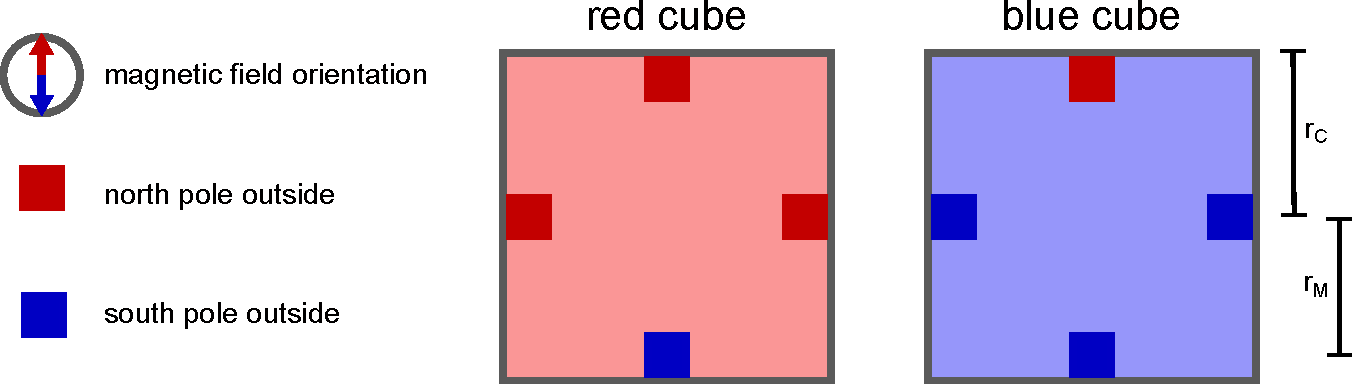
\includegraphics[width=0.75\textwidth]{figures/magnetic_cubes.pdf}
	\caption[Top-down view of the two magnetic modular cube types]{Simplified top-down view of the two magnetic modular cube types with their outward pointing magnet poles, illustrated as red and blue squares. Also visualizes the lengths $r_C$ and $r_M$ and the cardinal direction vectors of all cube faces.}
	\label{fig:magnetic_cubes}
\end{figure}

\begin{figure}
	\centering
	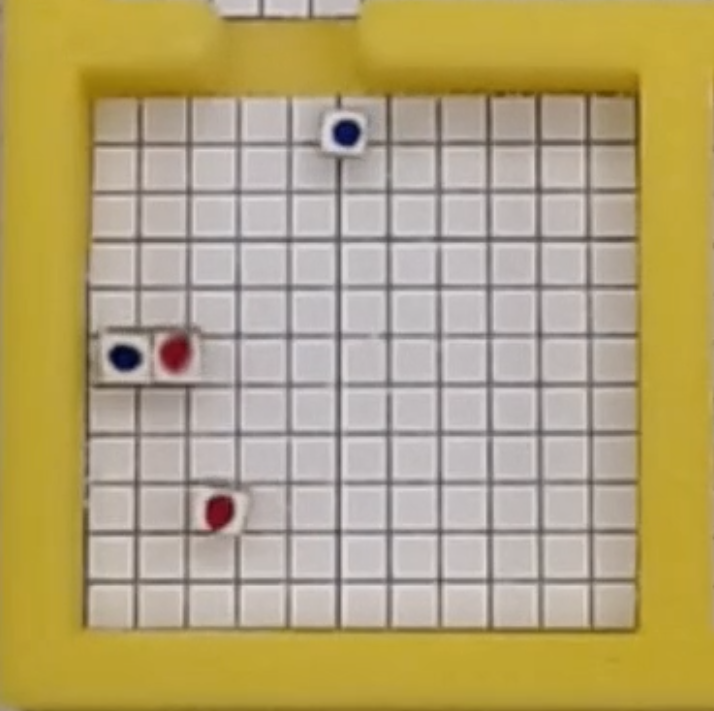
\includegraphics[width=0.5\textwidth]{figures/real_mmcs.png}
	\caption[Picture of magnetic modular cubes in real workspace]{Magnetic modular cubes with 2.8 mm edges in a real workspace. Picture was taken from a video made by A. Bhattacharjee showing the assembly of a four cube polyomino.}
	\label{fig:real_mmcs}
\end{figure}


The magnetic modular cubes are cube-shaped bodies embedded with permanent magnets on the four side faces.
The magnets have different orientations of their north and south pole. 
One pole is always pointing outward and the other straight to the center of the cube.
The magnet at the front face has its north pole pointing outwards and the magnet at the back its south pole.
These two magnets ensure that the cube is always aligned with the global magnetic field and this orientation holds true for both cube types.
The two other side faces must have the same outwards pointing pole, so that this axis does not provide a magnetic torque.

In fact, this is the reason a distinct definition of front, back and side is even possible.
Since the front is always pointing to the north pole of the magnetic field, we also call it the north face, or north edge in two dimensions, and all the other faces can also be called by their corresponding cardinal direction.
For each face we define a vector $\vec{e} \in \{ \vec{N},\vec{E},\vec{S},\vec{W}\}$ with $\lVert \vec{e} \rVert = 1$ pointing in the cardinal direction of the magnetic field.
For simplification we refer to magnets by their outwards pointing pole in further sections.

Furthermore, two different cube types are defined:
Either both side magnets point out their north pole, these cubes are called red cubes, or they point out their south pole, which is then called a blue cube.
\autoref{fig:magnetic_cubes} shows a top-down view of the two cube types with all the outwards pointing magnet poles.
A compass always shows the orientation of the magnetic field in our illustrations.

Magnetic Modular Cubes can be constructed in different sizes and ways. For more technical details and length measurements, we refer to the original paper \cite{Bhattacharjee2022}.
In \autoref{fig:real_mmcs} magnetic modular cubes with 2.8 mm edges can be seen in a real workspace.
Two important lengths that we use for planning and simulating are the cube radius $r_C$ and the magnet radius $r_M$ (also illustrated in \autoref{fig:magnetic_cubes}).
$r_C$ is one half-length of a cube face and $r_M$ is the distance from the center of the cube to the center of the magnet.



\section{Workspace and Configuration}

\begin{figure}
	\centering
	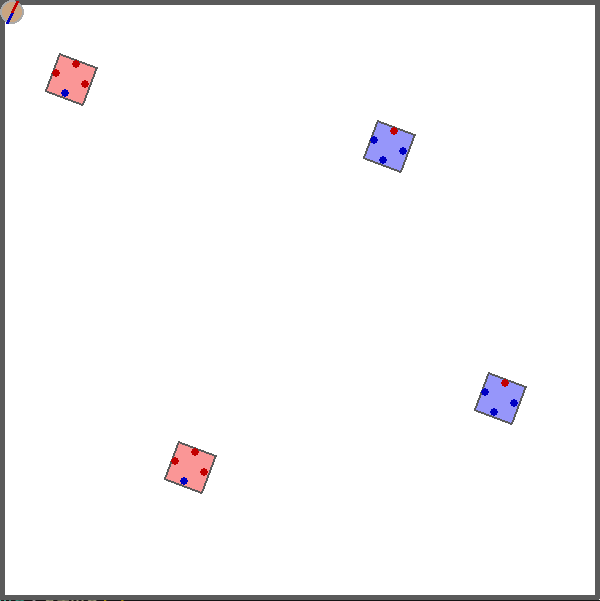
\includegraphics[width=0.45\textwidth]{figures/workspace_config.png}
	\caption[Workspace with a configuration of four magnetic modular cubes]{Rectangular workspace with a configuration of four magnetic modular cubes. All cubes have the same orientation as the magnetic field, indicated by the compass in the top-left corner.}
	\label{fig:workspace_config}
\end{figure}

Magnetic modular cubes could theoretically be placed and maneuvered on any 2-dimensional plane with numerous obstacles, as long as you can surround the workspace with a time varying magnetic field.
The magnetic field should be able to point in any direction specified by angles of latitude and longitude, so that the cubes can operate in all desired motion modes.
Because the motion planning problem of self-assembling target shapes in the special Euclidean group is hard enough without considering obstacles and arbitrary workspace shapes, this thesis limits itself to a rectangular workspace with no internal obstacles.
The workspace is bounded by surrounding walls, which are the only objects that could be considered as obstacles in classical motion planning.
However, we do not assume a fixed size, as long as the workspace stays finite and rectangular.

For planning we work in the configuration space of the 2-dimensional special Euclidean group $SE(2) = \mathbb{R}^2 \times \mathbb{S}^1$.
When only considering one cube, the group consists of the position in $\mathbb{R}^2$ and an orientation $\mathbb{S} = [0,2\pi)$ \cite{LaValle2006}.
When working with $n$ cubes, the dimension of our configuration space increases to $\mathbb{R}^{2n} \times \mathbb{S}^1$.
Note that we can still assume only one orientation for $n$ cubes, because we are working with a global magnetic field orienting all cubes the same way.
We assume that eventually all cubes align with the global magnetic field and only consider static configurations.
Future work could examine the dynamic configuration, which would enable faster motion planning, but a more complex planning problem.
\autoref{fig:workspace_config} shows a configuration with four cubes in the workspace.
It is irrelevant which exact physical cube is at which position as long as they are the same type, so switching the positions of the two red cubes in \autoref{fig:workspace_config} would lead to the same configuration as before.

\section{Polyominoes}
\label{sec:polys}

\begin{figure}
	\centering
	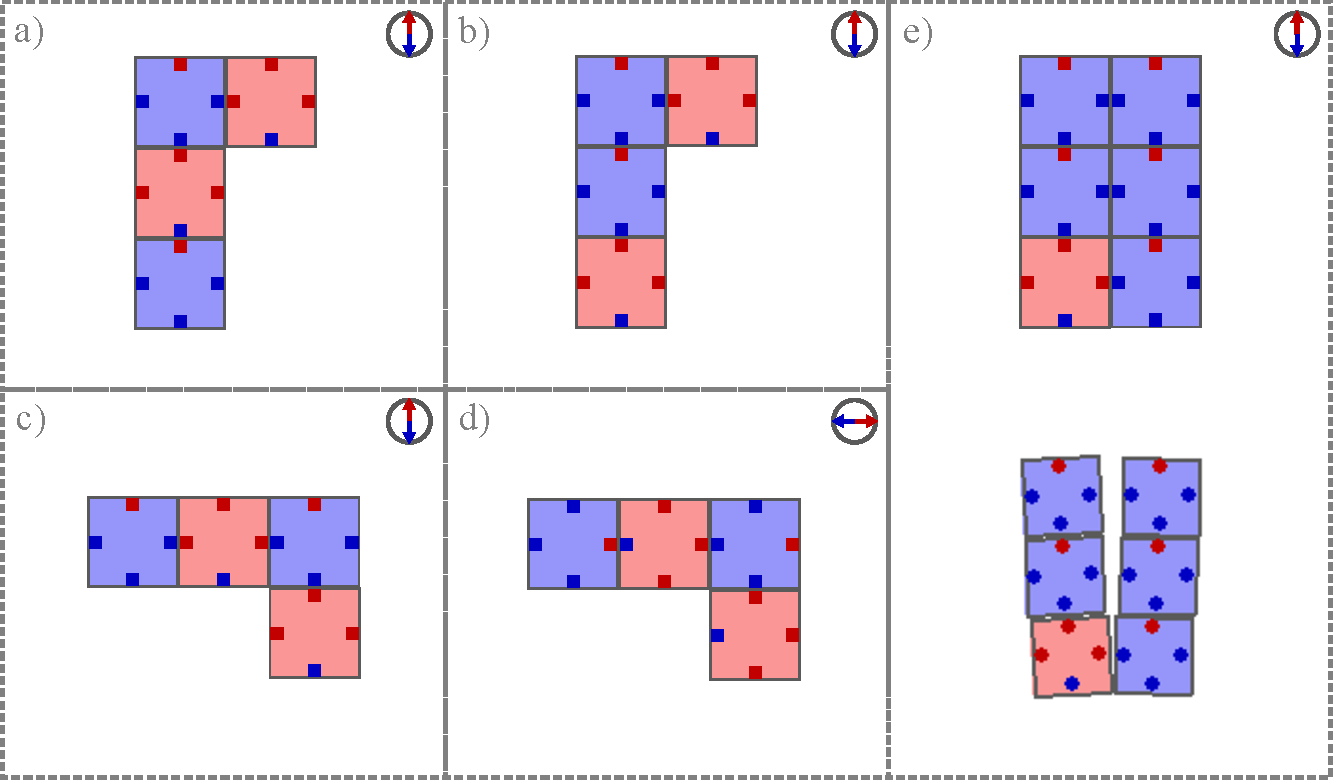
\includegraphics[width=0.65\textwidth]{figures/polyominoes.pdf}
	\caption[Examples of Polyominoes and their equality]{Examples of polyominoes and their equality. a) and d) are equal, only the magnetic field changed its orientation. a) and c) are not equal, they have the same shape, but it is rotated. a) and b) are also not equal because of different cube types in the same shape. e) shows an invalid polyomino in its grid representation (top) and how it behaves in the simulation (bottom).}
	\label{fig:polyominoes}
\end{figure}

The embedded magnets not only align the cube with the magnetic field, they also allow cubes to self-assemble into polyominoes.
Two cube faces can connect if their magnets have opposite polarities.
Because of this and the alignment with the magnetic field, cubes can either be connected at north and south faces, or east and west faces, if the cubes are not the same type.
A \textit{polyomino} is a set of uniformly sized cubes on a 2-dimensional grid.
Because we work with arbitrary positions and orientations the grid alignment does not hold true for multiple polyominoes in the workspace, but for each polyomino on its own the cubes can be represented in a local coordinate system with position $(x,y)$, $x,y \in \mathbb{Z}$ \cite{Lu2021}.

We consider \textit{fixed polyominoes}, meaning that two polyominoes are distinct if their shape or orientation are different \cite{Lu2021}.
The magnetic field always provides an orientation, so in \autoref{fig:polyominoes} a) and d) the polyominoes are equal, just the magnetic field is rotated.
Conversely, the polyominoes in \autoref{fig:polyominoes} a) and c) are the same shape but with a different rotation under the same magnetic field orientation, so they are not equal.
Furthermore, two polyominoes are only equal if all the cubes at equal positions are the same type.
The polyominoes in \autoref{fig:polyominoes} a) and b) are not equal because the cube types differ.
It is possible that a workspace contains multiple equal polyominoes.
In that case, we refer to them as being the same polyomino-type, instead of calling them equal, since it is important to differentiate between physical polyominoes with different positions.

The size of a polyomino is the number of cubes it consists of.
Because it is easier to view all structures in the workspace as a polyomino, single cubes are often referred to as trivial polyominoes with size 1.
Although it is not possible to connect cubes of same type at east and west faces, the magnetic modular cubes can assemble structures like the one shown in \autoref{fig:polyominoes} e).
The connection of the bottom two cubes is strong enough to hold the structure together, even though the four blue cubes on the top repel each other.
The resulting polyomino in its grid representation has two east-west connections between cubes the same type and is therefor marked as an invalid polyomino.


\section{Motion Modes}
\label{sec:motion}

\begin{figure}
	\centering
	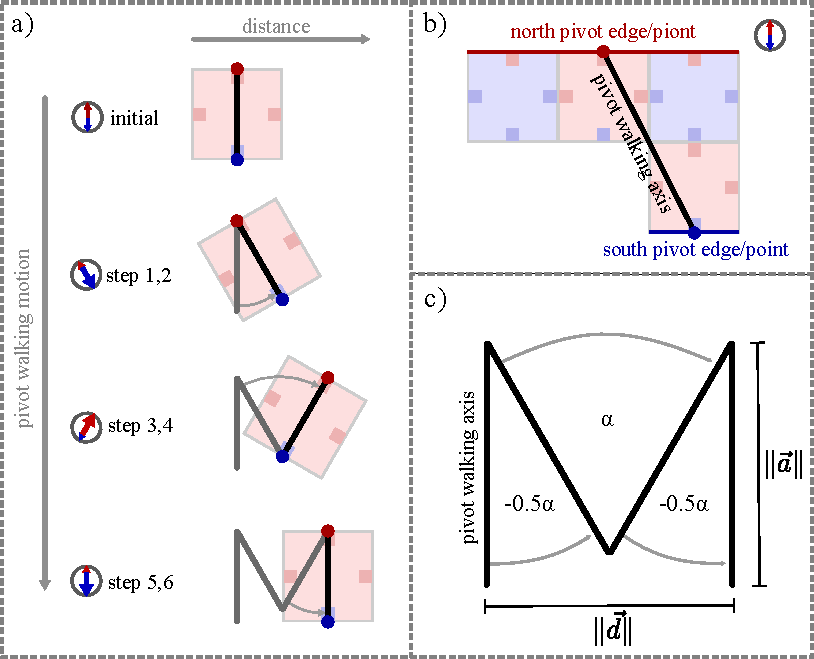
\includegraphics[width=0.80\textwidth]{figures/pivot_walking.pdf}
	\caption[Illustration of the pivot walking motion]{This figure describes the pivot walking motion in detail. a) shows the six pivot walking steps for a single red cube. You can see the orientation of the magnetic field (bigger arrow indicates elevation, so in step 1,2 the south pole is raised in the air). In b) an example polyomino with its pivot axis, edges and points is shown. c) illustrates the rotation of the pivot axis labeled with all the pivot walking parameters.}
	\label{fig:pivot_walking}
\end{figure}

In \cite{Bhattacharjee2022} three motion modes are presented. Rotation, pivot walking, and rolling.

If the magnetic field orientation lays in the plane of the workspace and rotates without any inclination the rotation is performed around the center of mass for all polyominoes and we consider this motion a normal rotation.

Rotating the magnetic field perpendicular to the workspace plane, cubes can roll forwards or backwards.
This rolling motion becomes problematic for self-assembly, because the top and bottom face of the cube, which contain no magnets, can become a side face.
Because rotation and pivot walking are sufficient to reach any position in the workspace, we do not consider rolling in our simulation and planning algorithms.

When elevating the magnetic field orientation by lifting up the south pole slightly, all polyominoes will pivot on the north face bottom edges of their most north-placed cubes.
Pulling up the north pole does the opposite. The polyominoes will pivot on the south face bottom edges of their most south-placed cubes.
The sum of all these cube edges is called the north or south pivot-edge and by keeping the magnetic field elevated and rotating around the normal vector of the workspace plane, the polyominoes will rotate around the center point of their pivot-edge.
This point is called the north or south pivot-point.
All these edges and points are illustrated in \autoref{fig:pivot_walking} b).


\paragraph{pivot walking:}

\begin{figure}
	\centering
	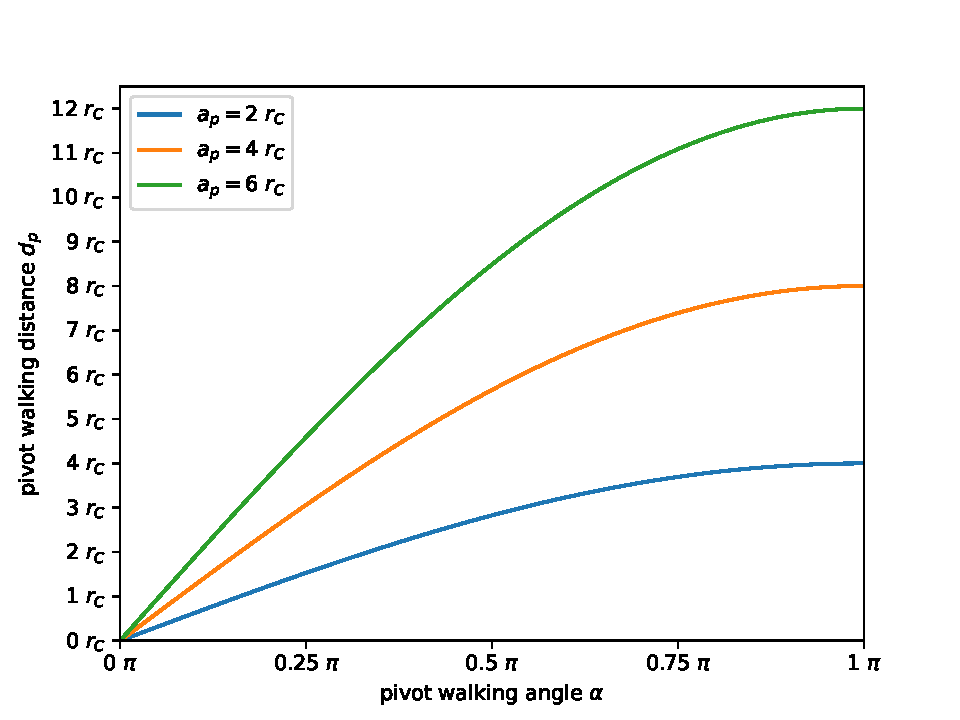
\includegraphics[width=0.60\textwidth]{figures/plots/pivot_walking_angle.pdf}
	\caption[Functions of $d_p$ based on $\alpha$ for different $a_p$]{Functions of the pivot walking distance $d_p$ based on pivot walking angle $\alpha$ for different pivot walking axes with length $a_p$. Lengths are given in multiples of cube radius $r_C$.}
	\label{fig:pw_angle_plot}
\end{figure}

\begin{figure}
	\centering
	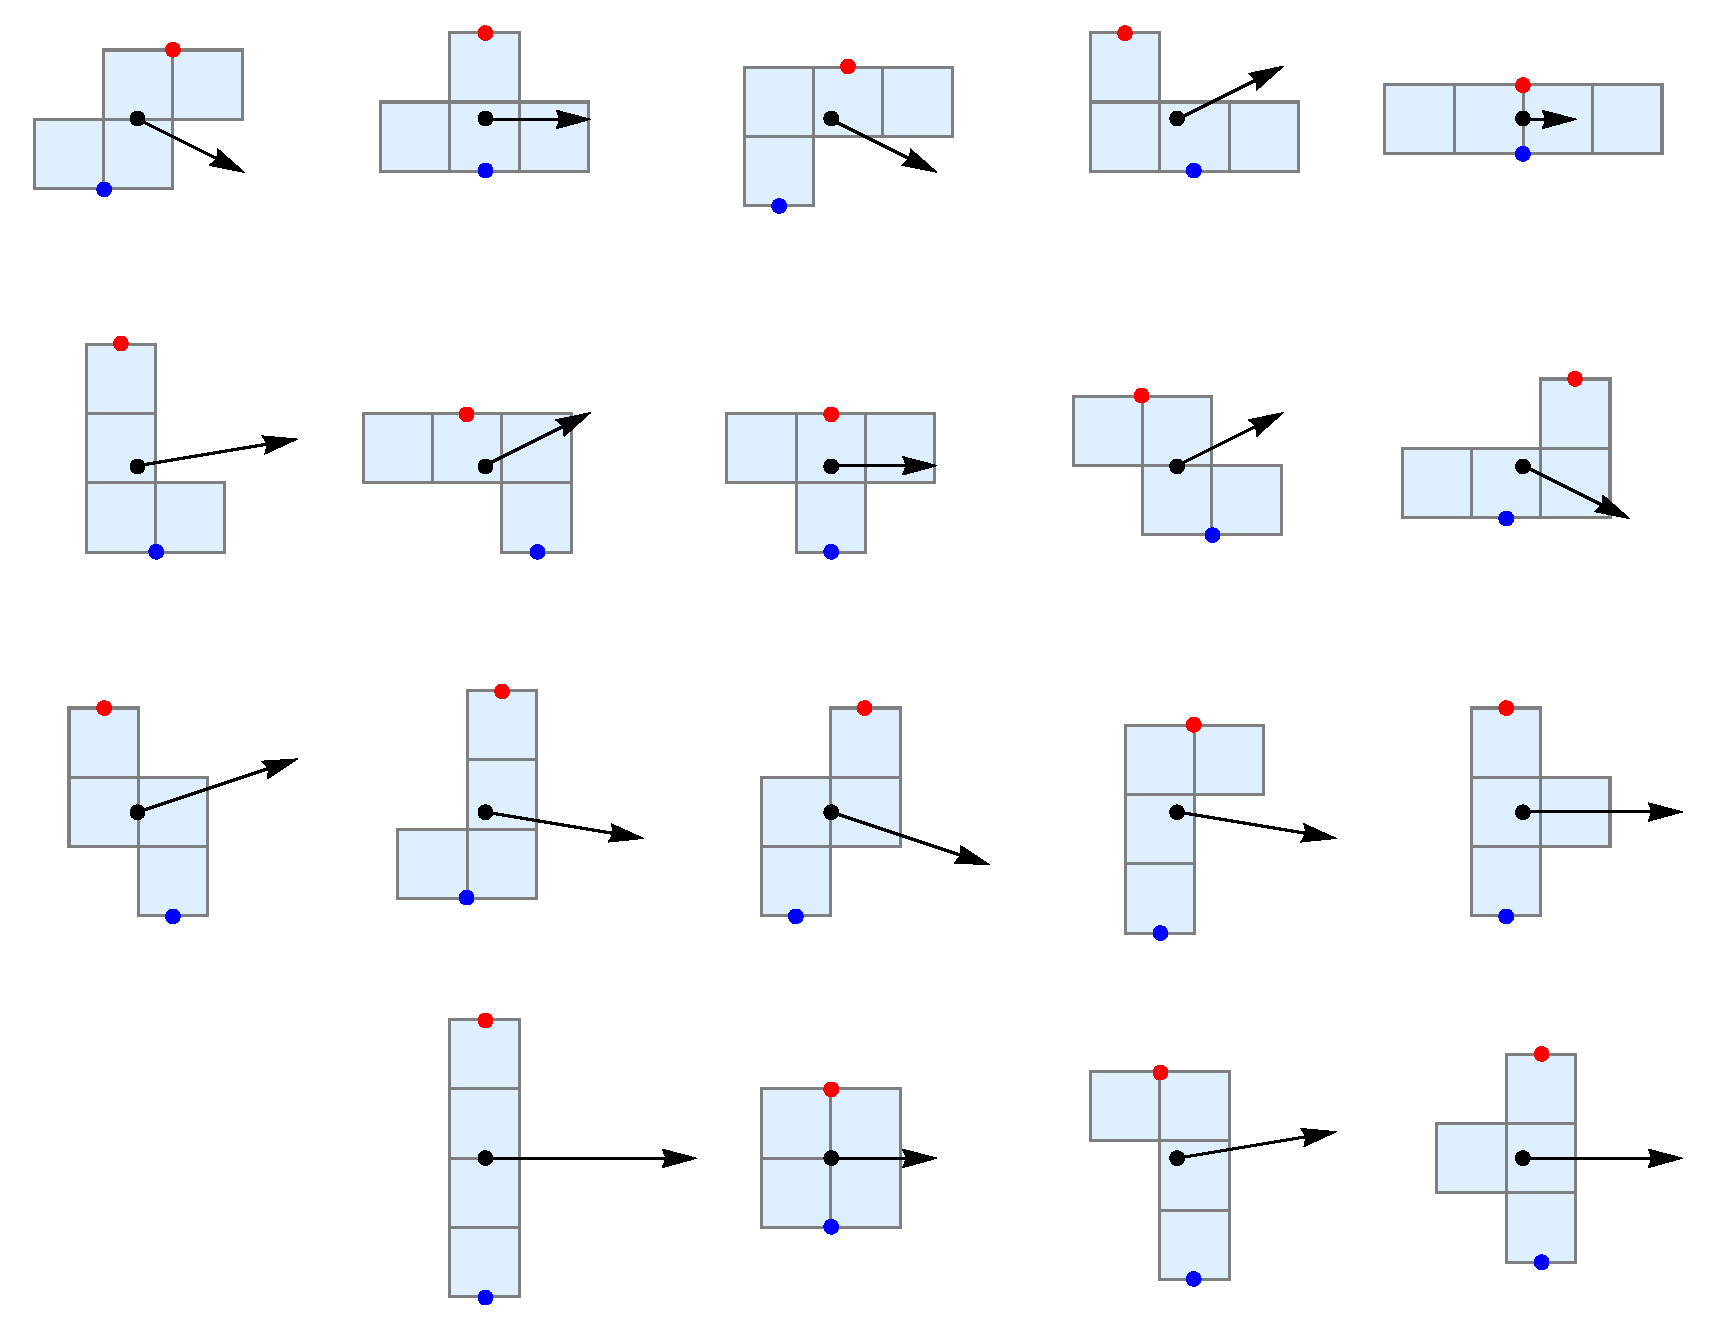
\includegraphics[width=0.70\textwidth]{figures/displacement_pivot_walking.pdf}
	\caption[Polyomino shapes with different displacement vectors]{All 19 four-cube polyomino shapes with their displacement vector $\vec{d}$ for one pivot walking cycle with $\alpha = \frac{\pi}{4}$. $\vec{d}$, drawn with a black arrow from its center of mass. North and south pivot point are drawn as red and blue dots.}
	\label{fig:displacement_pivot_walking}
\end{figure}

Not rotating around the center of mass is important for pivot walking.
In the first step of a pivot waking cycle, the magnetic field is elevated to let the polyomino pivot on its north pivot edge.
As a second step a rotation of $-\frac{1}{2} \cdot \alpha$ is performed around the north pivot point.
$-\pi \leq \alpha \leq \pi$ is the pivot walking angle.
For step 3 and 4 the elevation changes to its opposite to perform a rotation of $\alpha$ around the south pivot point.
Step 5 and 6 are equal to 1 and 2 and will bring the polyomino back to its original orientation.
You can see the pivot walking cycle steps in \autoref{fig:pivot_walking} a) and have a closer look at its parameters in \autoref{fig:pivot_walking} c).

After one pivot walking cycle, the polyomino has moved by a displacement vector $\vec{d}$ with $\lVert \vec{d} \rVert = d_p$, so $d_p$ is the distance the polyomino moved.
The direction and length of $\vec{d}$ changes with the shape of the polyomino.
The movement is always perpendicular to the pivot walking axis $\vec{a}$ with $\lVert \vec{a} \rVert = a_p$, which is the vector between the north and the south pivot point, visualized in \autoref{fig:pivot_walking} b).
$d_p$ can be calculated as
\begin{equation}
d_p = 2 \cdot \sin\left(\frac{1}{2} \cdot \alpha \right) \cdot a_p \,.
\end{equation}
\autoref{fig:pw_angle_plot} shows functions for this equation based on $\alpha$ for different $a_p$.
To calculate $\vec{d}$ you can take the perpendicular of $\vec{a}$ and scale it to the length $d_p$.

When a big $\alpha$ is chosen according to amount, $d_p$ becomes also bigger, but the polyomino needs more space to the north and south to perform the rotations.
For better maneuvering smaller values of $\alpha$ are preferable.
There is a strong deviation of length and direction of the displacement for different polyomino shapes.
Doing a pivot walking motion might not move two polyominoes in the same direction.
\autoref{fig:displacement_pivot_walking} shows all 19 four-cube polyomino shapes with their displacement vectors.
There are still two options for pivot walking, depending on a negative or positive value of $\alpha$.
You can walk left, in the direction of the west-faces, or right, in the direction of the east-faces.
Although the polyomino actually moves in the direction of $\vec{d}$, we can still say that a pivot walk right moves to the east, because $\left| \angle \left( \vec{E}, \vec{d} \right) \right| < \frac{\pi}{2}$.
We call these two options the pivot walking direction $\vec{w} \in \{\vec{E}, \vec{W}\}$.

	\chapter{Local Planner}
\label{chap:local}

This chapter is about the local planner that will be used for motion planning on a global scale in \autoref{chap:global}.
A local planner only focuses on simple motion task.
Possible tasks could be developing a plan that moves a polyomino from one position to another, or even simpler, to develop a plan for one pivot walking cycle.
Considering the problem of self-assembly on a global scale, the initial and goal configuration of local plans should differ in the set of polyominoes they contain.
Our local planner takes two cubes $c_\mathcal{A}$ and $c_\mathcal{B}$ out of the polyominoes $\mathcal{A}$ and $\mathcal{B}$ and attempts to establish a connection at a valid edge-pair $(e_\mathcal{A}, e_\mathcal{B})$.
A successful local plan guaranties a change of polyominoes in the workspace.

For this, the local planner makes use of our simulator from \autoref{chap:sim} in a closed-loop manner.
This means that the configuration of the workspace can be observed at any time and the actions can be adjusted accordingly.
The local planner works with position and orientation of cubes and polyominoes provided by the simulator.
The distance between two cubes is the Euclidean distance $d(c_\mathcal{A}, c_\mathcal{B}) = \lVert p_{c_{\mathcal{A}}} - p_{c_{\mathcal{B}}}\rVert$ between the cube centers $p_{c_\mathcal{A}}$ and $p_{c_\mathcal{B}}$.
In a real application of Magnetic Modular Cubes a camera, able to track cubes in the workspace, could to used to retrieve the necessary information. 

The following Sections \ref{sec:align} to \ref{sec:plan} explain the techniques used in the local planning algorithm of \autoref{sec:local_algo}.


\section{Aligning Cubes}
\label{sec:align}

\begin{figure}
	\centering
	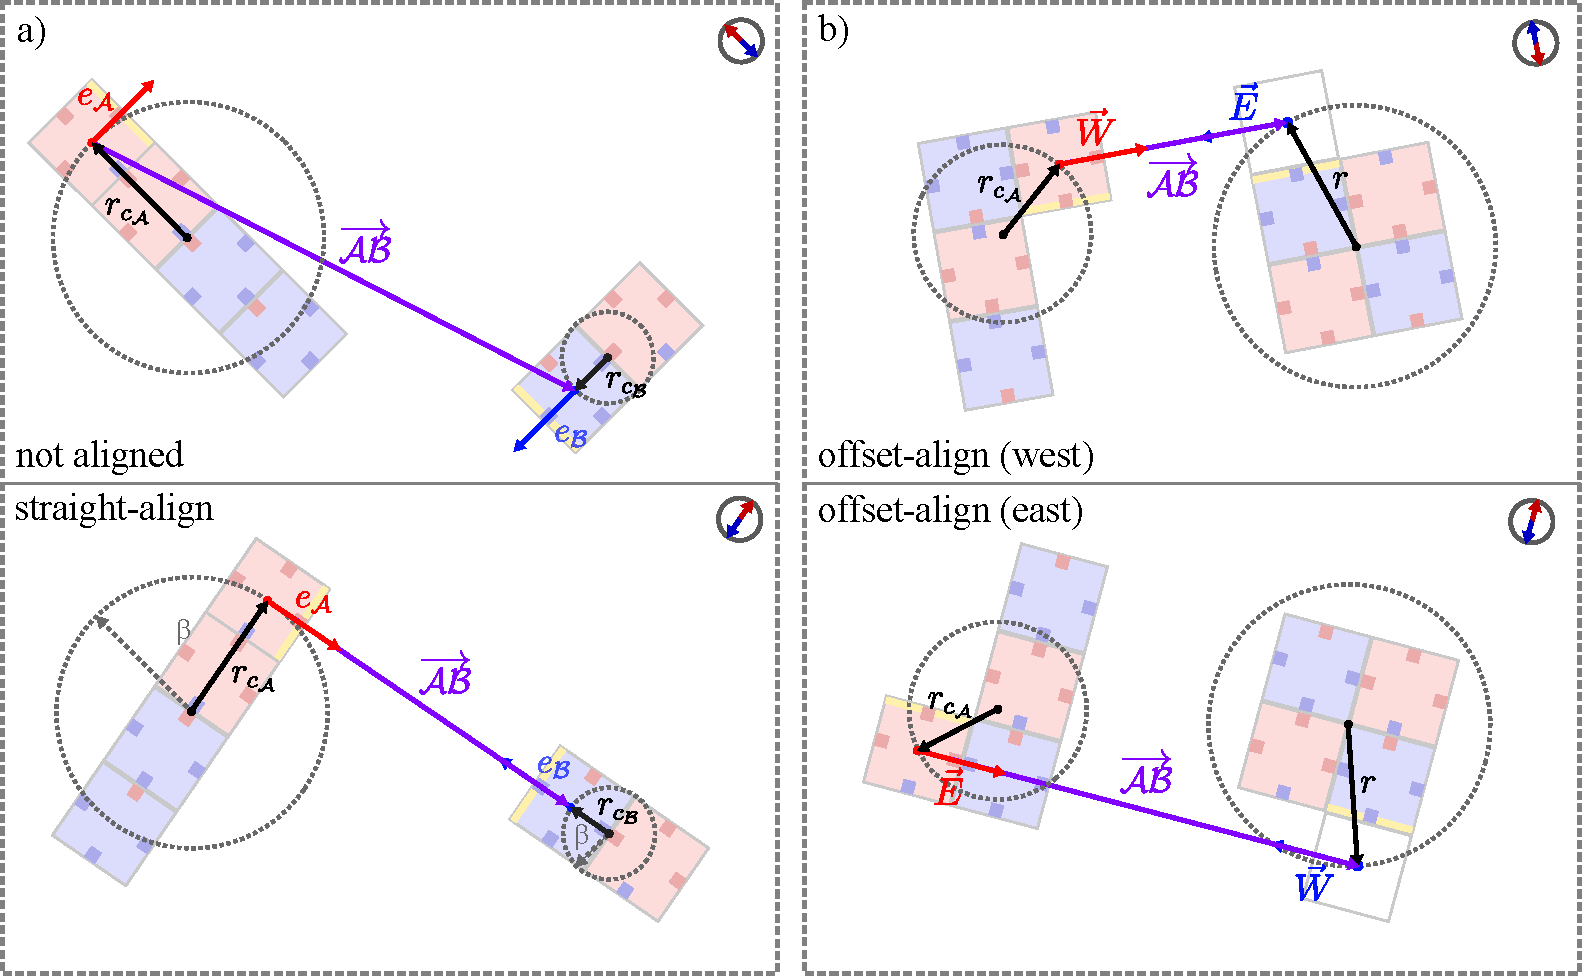
\includegraphics[width=0.90\textwidth]{figures/aligning.pdf}
	\caption[Illustration of straight- and offset-aligning]{Examples illustrating straight- and offset-aligning. The edges to be connected are marked yellow. a) shows two not aligned polyominoes (top) and the result of a straight-align (bottom). In b) the results of the two approaches for offset-aligning are shown. $c_\mathcal{A}$ was aligned with its west edge (top) and with its east edge (bottom).}
	\label{fig:aligning}
\end{figure}

\begin{figure}
	\centering
	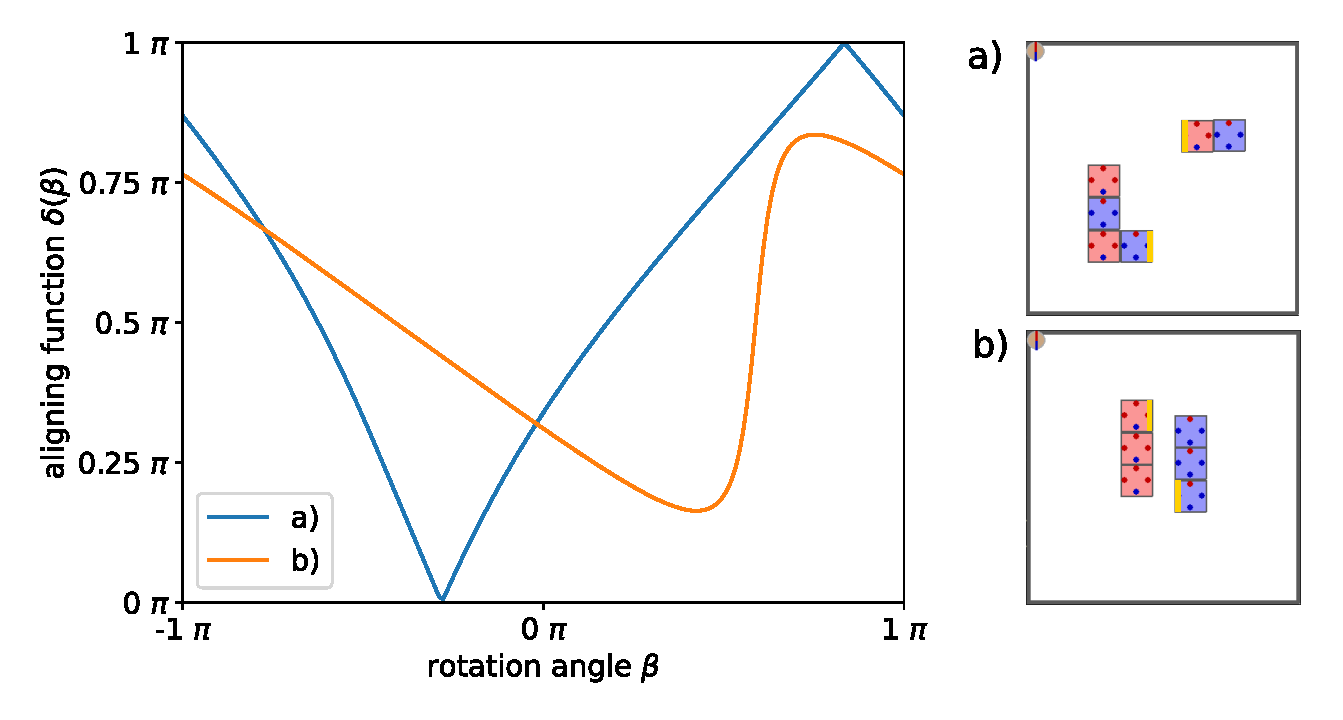
\includegraphics[width=0.8\textwidth]{figures/plots/aligning_function.pdf}
	\caption[Examples of aligning functions $\delta(\beta)$]{Two examples of the aligning function $\delta(\beta)$ for different configurations of polyominoes. The edges about to be aligned are marked yellow. The cubes are perfectly aligned, when $\delta(\beta) = 0$. This can be seen for example a) at $\beta \approx -0.28\pi$. Rotating the magnetic field around this angle of $\beta$, would align the cubes. In example b) $\delta(\beta)$ never gets zero. Perfect alignment is not possible, because the polyominoes are to close.}
	\label{fig:aligning_plot}
\end{figure}

To establish a connection between two polyominoes $\mathcal{A}$ and $\mathcal{B}$, the connection-cubes $c_\mathcal{A}$ and $c_\mathcal{B}$ with their connection-edges $e_\mathcal{A}$ and $e_\mathcal{B}$ need to be aligned in the correct way.
When $\mathcal{A}$ is rotated without magnetic field elevation, a cube center rotates in a circle around the center of mass of its polyomino $p_\mathcal{A}$.
The vector $r_{c_\mathcal{A}} = p_{c_\mathcal{A}} - p_\mathcal{A}$ is the radius of this rotation-circle.
When also considering $\mathcal{B}$, a rotation of the magnetic field rotates $r_{c_\mathcal{A}}$ and $r_{c_\mathcal{B}}$ by the same angle $\beta$.
The goal is to find this angular difference $\beta$, so that the cubes are aligned.
There are two different approaches for alignment: Straight-aligning and offset-aligning.

\paragraph{Straight-Aligning}

For straight aligning we define a vector $\overrightarrow{\mathcal{A}\mathcal{B}} = p_{c_\mathcal{B}} - p_{c_\mathcal{A}}$ pointing form $c_\mathcal{A}$ to $c_\mathcal{B}$.
The alignment is done when $e_\mathcal{A}$ points in the same direction as $\overrightarrow{\mathcal{A}\mathcal{B}}$, so $\angle \left( e_\mathcal{A}, \overrightarrow{\mathcal{A}\mathcal{B}} \right) = 0$.
Consequently $\angle \left( e_\mathcal{B}, \overrightarrow{\mathcal{A}\mathcal{B}} \right) = \pi$, since $e_\mathcal{A}$ and $e_\mathcal{B}$ have to be opposite edges for a connection.

\autoref{fig:aligning} a) illustrates a straight-align for an east-west connection with all its parameters.
The two polyominoes could now theoretically pivot walk together and connect at the desired edges.
Straight-aligning is always used for east-west connections, but we also use it for north-south connection in one special case. More on that in \autoref{sec:plan}.

\paragraph{Offset-Aligning}

When considering north-south connections we need to align with an offset, so that the cubes can be moved together from either east or west direction.
We again define $\overrightarrow{\mathcal{A}\mathcal{B}} = \left( d_\textit{offset} \cdot e_\mathcal{B} + p_{c_\mathcal{B}} \right) - p_{c_\mathcal{A}}$, but this time an offset $d_\textit{offset}$ is added to $p_{c_\mathcal{B}}$ in the direction of $e_\mathcal{B}$, so $\overrightarrow{\mathcal{A}\mathcal{B}}$ points from $p_{c_\mathcal{A}}$ to a position above or below $p_{c_\mathcal{B}}$.
In a perfect world $d_\textit{offset} = 2 \cdot r_C$ is exactly one cube length, but to avoid failures when moving together, we give the alignment a bigger offset.
Instead of pointing $e_\mathcal{A}$ in the same direction as $\overrightarrow{\mathcal{A}\mathcal{B}}$, we now have two options:
Either solving $\angle \left( \vec{E}, \overrightarrow{\mathcal{A}\mathcal{B}} \right) = 0$ or $\angle \left( \vec{W}, \overrightarrow{\mathcal{A}\mathcal{B}} \right) = 0$, depending on if we want to move $\mathcal{A}$ in east direction, or in the west direction towards $\mathcal{B}$.
You can see the two options for offset-aligning in \autoref{fig:aligning} b).

\subsection{Solving Alignment}

For calculating angular difference we use the dot-product
\begin{equation*}
\angle (a,b) = \frac{a \cdot b}{\lVert a \rVert \lVert b \rVert} \,,
\end{equation*}
with $a,b \in \mathbb{R}^2$. This way the difference is always positive, which is beneficial in the case of alignment.
We define a function for straight-aligning based on the rotation angle $\beta$, where both $e_\mathcal{A}$ and $\overrightarrow{\mathcal{A}\mathcal{B}}$ are rotated accordingly.
\begin{equation}
\delta(\beta) = \angle \left( \mathbf{R}_\beta e_\mathcal{A}, \, \left( \mathbf{R}_\beta r_{c_\mathcal{B}} + p_\mathcal{B} \right) - \left( \mathbf{R}_\beta r_{c_\mathcal{A}} + p_\mathcal{A} \right)\right) \,.
\end{equation}
$\mathbf{R}_\beta$ is a rotation matrix used for rotating vectors by $\beta$.
For an offset-align the function would be
\begin{equation}
\delta(\beta) = \angle \left( \mathbf{R}_\beta e, \, \left( \mathbf{R}_\beta r + p_\mathcal{B} \right) - \left( \mathbf{R}_\beta r_{c_\mathcal{A}} + p_\mathcal{A} \right)\right) \,,
\end{equation}
with $e \in \{ \vec{E}, \vec{W}\}$ and $r = \left( d_\textit{offset} \cdot e_\mathcal{B} + p_{c_\mathcal{B}} \right) - p_\mathcal{B}$

Alignment is not always possible, so instead of solving $\delta(\beta) = 0$, the function is minimized.
\autoref{fig:aligning_plot} shows two example cases for $\delta(\beta)$.
In example b) $\delta(\beta)$ does not get zero, because the polyominoes are to close to ever reach perfect alignment.
Because $-\pi < \beta \leq \pi$, we can iterate through increasing values of $\beta$.
If a value close enough to zero is encountered, it can returned.
If not, the minimum of all the calculated values is returned.
This way we at least get as close to an alignment as possible.


\section{Moving Polyominoes Together}
\label{sec:walk_wait}

Pivot walking only allows the polyominoes to move left or right depending on $\vec{w}$.
If we want to connect an east face of polyomino $\mathcal{A}$ to a west face of polyomino $\mathcal{B}$, $\mathcal{A}$ has to walk into the east direction towards $\mathcal{B}$, or the other way around.

When $\mathcal{A}$ should be connected at a south face of $\mathcal{B}$, $\mathcal{A}$ can now walk into east or west direction towards $\mathcal{B}$, and $\mathcal{B}$ could again do the opposite.
We call this the \textit{slide-in direction} $\vec{m} \in \{\vec{E}, \vec{W}\}$, which states that $\mathcal{B}$ is positioned in direction $\vec{m}$ of $\mathcal{A}$.
Both slide-in directions can be archived in any configuration with offset-aligning from \autoref{sec:align}.
In \autoref{fig:aligning} b) you can see the difference the slide-in directions can make.
In this example, establishing a connection by letting $\mathcal{A}$ move towards $\mathcal{B}$ in west direction is possible, but by moving in east direction other cubes of the polyominoes are blocking the way.
In \autoref{sec:plan} we present a method for checking which slide-in directions are possible for two polyominoes. 

Since both polyominoes $\mathcal{A}$ and $\mathcal{B}$ perform pivot walking motions simultaneously, due to global control, a connection will most likely happen when one polyomino walks into a wall of the workspace boundary.
Connection can only happen in the middle of the workspace when one polyomino is faster than the other, meaning it has a greater pivot walking distance $\lVert \vec{d} \rVert$.

At a first glance it seems easy to move polyominoes together, after the connection-cubes are aligned, but in reality it becomes more difficult.
When a polyomino is continuously walking against a wall at any angle other than 90 degree, the polyomino will move alongside the wall.
In \cite{schmidt2020} research is done on how friction with boundary-walls under global control forces can be used to calculate the necessary motions for reaching a desired goal configuration, but friction forces depend greatly on material choices and are stochastic.

Another difficulty are different orientations of displacement vectors, since a pivot walking motion is actually performed in the direction of the displacement $\vec{d}$ and not directly in direction of $\vec{w}$.
It is mathematically possible to calculate the right orientation of the magnetic field to result in a collision after a certain number of pivot walking cycles for both polyominoes with different displacement directions, even at desired edges, but it is not guaranteed that this collision-point is within the workspace boundaries.
In that case the calculation of friction and displacement have to be combined together with other factors like polyominoes blocking each other or changing their shape during movement.

This is fairly complex and recalculating would be necessary in many situations, so we choose a simpler dynamic approach.
We estimate the pivot walking cycles necessary until $c_\mathcal{A}$ moved to the original position of $c_\mathcal{B}$ with
\begin{equation}
\#\textit{walks} = \left\lceil \frac{d(c_\mathcal{A}, c_\mathcal{B})}{\lVert \vec{d}_\mathcal{A} \rVert} \right\rceil \,.
\end{equation}
We then only walk $\frac{\#\textit{walks}}{2}$ and re-align the cubes.
When $c_\mathcal{A}$ and $c_\mathcal{B}$ are near enough for magnetic forces to act, we frequently wait a short period to let magnetic attraction pull $e_\mathcal{A}$ and $e_\mathcal{B}$ together.
This will automatically adjust the alignment, but for even more precision we decreased the pivot walking angle $\alpha$ when in close proximity.

\section{Plan and Failures}
\label{sec:plan}

A plan is a sequence of actions $A = a_1, ... , a_k$ that when applied to an initial configuration $g_\textit{init}$, leads to a goal configuration $g_\textit{goal}$.
Two plans can be concatenated when the goal of the first matches with the initial configuration of the second.
That way multiple local plans can be connected to form a global plan.
We define a metric to compare and evaluate plans based on rotational cost of its actions.
We only consider longitude magnetic field rotations, not latitude elevation.
Let $a_i$ be a normal rotation of angle $\beta$, then $\text{cost}(a_i) = |\beta|$.
If it is a pivot walking motion, then $\text{cost}(a_i) = |2\alpha|$.
The cost for the plan is the sum of the costs of all its actions
\begin{equation}
\text{cost}(A) = \sum_{i=1}^{k} \text{cost}(a_i) \,.
\end{equation}
A local plan is successful if $g_\textit{goal}$ contains a polyomino with the desired connection of $c_\mathcal{A}$ and $c_\mathcal{B}$ at $(e_\mathcal{A}, e_\mathcal{B})$.
The plan-state $s$ describes if a plan is successful or not.
There are several reasons the local planner might fail to develop a plan:

\paragraph{Impossible Connection}

Most failures occur, because it is not possible to connect the polyominoes.
First of all, $e_\mathcal{A}$ and $e_\mathcal{B}$ need to be free, so no other cube is already connected to them.
Even if both edges are free, other cubes then $c_\mathcal{A}$ and $c_\mathcal{B}$ can prevent a connection.
By connecting two polyominoes in one local discrete coordinate-system, for all cubes $c_1$, $c_2$ with coordinates $(x_1, y_1)$, $(x_2, y_2)$: $\left|x_1 - x_2\right| < 1$ and $\left|y_1 - y_2\right| < 1$ should hold true.
If two positions are equal, we call this an overlap, which prevents the connection.
Of course, a connection is never possible if $e_\mathcal{A}$ and $e_\mathcal{B}$ are part of the same polyomino and not already connected.

All these conditions are easy to check in a discrete way before even starting to plan, but connections with other polyominoes during planning can invalidate those pre-checked conditions.
Because of this, frequently re-checking them is necessary.

\paragraph{Impossible Slide-In}

Even if a connection in a common local coordinate-system is possible, the polyominoes need to slide in from east or west dsirection.
Other cubes can again prevent this by blocking the way for an easy slide-in.
We can verify both slide in directions $\vec{m}$ in a common local coordinate system.
This discrete check assumes exact movement from east or west direction.
Because of different displacement directions, we know this is not true, but it is a reasonable approximation.
Research on assembling a polyomino out of two parts by moving one part towards the other without collision, was done by Agarwal et al. \cite{agarwal2021}. 

When pre-checking this condition, we can state failure if both directions are not possible.
Otherwise, we can align with respect to the valid slide-in direction, or try out both, if both are possible.
Again, this condition needs to be re-checked frequently, due to changing polyominoes.

\paragraph{Polyominoes being Stuck}

Polyominoes can get stuck in corners or on walls of the workspace.
In this state it is not possible to decrease the distance of $\mathcal{A}$ and $\mathcal{B}$ by pivot walking.
We can identify this state when the positions  of both $c_\mathcal{A}$ and $c_\mathcal{B}$ do not change after a certain amount of pivot walking motions.

When stuck while trying to establish a north-south connection, a straight-align, instead of an offset-align, can resolve the situation.
Success depends on the distance of the cubes after straight-aligning.
If the distance is too big for magnetic forces to act, failure is reported.
If the cubes are close enough the local planner waits until magnetic attraction connects $e_\mathcal{A}$ and $e_\mathcal{B}$.


\paragraph{Connecting in Caves}

\begin{figure}
	\centering
	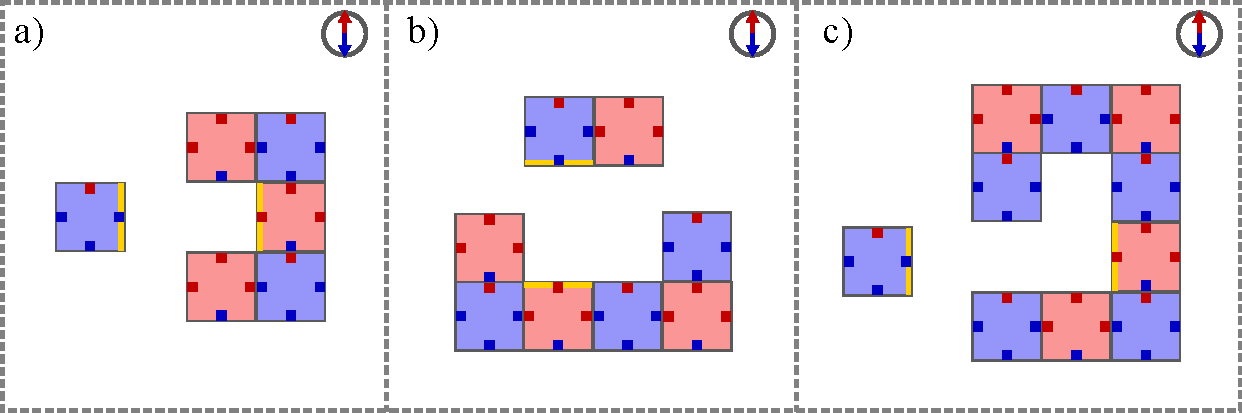
\includegraphics[width=0.80\textwidth]{figures/caves.pdf}
	\caption[Examples for connecting polyominoes into caves]{Three different examples for connecting polyominoes into caves. a) and b) show one-cube-deep caves (a) east-west and b) two-cube-wide north-south). c) illustrates a two-cube-deep east-west cave. The edges to be connected are marked yellow.}
	\label{fig:caves}
\end{figure}

Connecting two polyominoes where one of the connection-faces is located inside a cave is a difficult task in the continuous world.
We differentiate between east-west and north-south located caves.
Furthermore, a cave can be of certain depth and width measured in multiples of $2 r_C$.
\autoref{fig:caves} shows examples for caves with varying depths and widths.

Caves only become problematic when the polyomino to be inserted has the same width as the cave, shown in \autoref{fig:caves} b).
Connecting into a cave with a depth of more than $2 r_C$ is not possible.
For instance, when inserting the blue single cube into the polyomino in \autoref{fig:caves} c), the blue cube would connect with north and south faces of the polyomino before even reaching the full depth of the cave.
But even caves with depth $2 r_C$ are hard to handle.

Inserting into a cave can be done by pivot walking.
This only works for east-west caves, or by letting magnetic forces attract $e_\mathcal{A}$ and $e_\mathcal{B}$.
Relying on magnetic forces alone seem promising, since it would work for both cave types, but in reality not only the forces of the connection-faces are present.
All the forces between other magnets prevent an easy insertion into the cave.
In our simulator the connection-face will be more attracted or repelled by faces outside the cave, then the once inside.
Pivot walking into east-west caves, even with small values for $\alpha$, has also a high failure rate because of other magnets.
The local planner states failure immediately when polyominoes should be connected in any cave-type.

\paragraph{Invalid Polyominoes}

Because construction of invalid polyominoes is hard to handle on a global scale, we already omit plans containing them in our local planner.
Failure is stated if an invalid polyomino is created at any point during planning.
We also pre-check (and frequently re-check) if the polyomino that will be created by establishing the connection would itself be invalid. 

\paragraph{Maximum Movement Capacity}

As a worst-case failure, we limit the amount of movement $\mathcal{A}$ and $\mathcal{B}$ are able to do.
Whenever a pivot walking motion is done, we sum up the distances $c_\mathcal{A}$ and $c_\mathcal{B}$ moved together.
We define a maximum movement capacity of $2\cdot(\text{width} + \text{height})$ dependent on the size of the workspace.
This capacity gives the polyominoes enough movement, so that both can move along a horizontal and vertical workspace boundary, which should be sufficient to establish a connection.

\section{Local Planning Algorithm}
\label{sec:local_algo}

\begin{algorithm}
	\caption{\scshape Align-Walk-Realign}
	\label{algo:local_algo}
	\begin{algorithmic}[1]
		\REQUIRE $c_\mathcal{A}$, $c_\mathcal{B}$, $e_\mathcal{A}$, $e_\mathcal{B}$, $\vec{w}$, $\vec{m}$, $g_\textit{init}$ 
		\ENSURE $(s, g_\textit{goal}, A)$ \COMMENT{state $s$ and actions $A$ leading to configuration $g_\textit{goal}$}
		\STATE $s \gets \text{undefined}$
		\STATE $g_\textit{goal} \gets g_\textit{init}$
		\STATE $A \gets \{\}$
		\STATE $\text{wait} \gets$ \TRUE
		\LOOP
			\IF[aligning straight or with offset]{$e_\mathcal{A} \in \{\vec{E},\vec{W}\}$}
				\STATE $a \gets \text{\scshape Align-Straight}(c_\mathcal{A}, c_\mathcal{B}, e_\mathcal{A})$
			\ELSE
				\STATE $a \gets \text{\scshape Align-Offset}(c_\mathcal{A}, c_\mathcal{B}, \vec{m}, e_\mathcal{B})$
			\ENDIF
			\STATE $g_\textit{goal} \gets \text{\scshape Simulate}(g_\textit{goal}, a)$
			\STATE $A \gets \text{\scshape Append}(A, a)$
			\STATE $s \gets \text{\scshape Update-State}(g_\textit{goal}, c_\mathcal{A}, c_\mathcal{B}, e_\mathcal{A}, \vec{m})$
			\IF[first time checking for failure or success]{$s \neq \text{undefined}$}
				\RETURN $(s, g_\textit{goal}, A)$
			\ENDIF
			\IF[wait or walk]{$\text{\scshape Critical-Distance}(c_\mathcal{A}, c_\mathcal{B})$ \AND wait}
				\STATE $a \gets \text{\scshape Wait}()$
				\STATE $\text{wait} \gets$ \FALSE
			\ELSE
				\STATE $a \gets \text{\scshape Walk}(c_\mathcal{A}, c_\mathcal{B}, \vec{w})$ \COMMENT{$a$ is $\frac{\#\textit{walks}}{2}$ actions (\autoref{sec:walk_wait})}
				\STATE $\text{wait} \gets$ \TRUE
			\ENDIF
			\STATE $g_\textit{goal} \gets \text{\scshape Simulate}(g_\textit{goal}, a)$
			\STATE $A \gets \text{\scshape Append}(A, a)$
			\IF[handle stuck condition]{$\text{\scshape Stuck}(c_\mathcal{A}, c_\mathcal{B})$}
				\STATE $a \gets \text{\scshape Align-Straight}(c_\mathcal{A}, c_\mathcal{B}, e_\mathcal{A})$ \COMMENT{do a straight aligne}
				\STATE $g_\textit{goal} \gets \text{\scshape Simulate}(g_\textit{goal}, a)$
				\STATE $A \gets \text{\scshape Append}(A, a)$
				\WHILE[let magnets attract until stuck again]{\NOT $\text{\scshape Stuck}(c_\mathcal{A}, c_\mathcal{B})$}
					\STATE $a \gets \text{\scshape Wait}()$
					\STATE $g_\textit{goal} \gets \text{\scshape Simulate}(g_\textit{goal}, a)$
					\STATE $A \gets \text{\scshape Append}(A, a)$
				\ENDWHILE
			\ENDIF
			\STATE $s \gets \text{\scshape Update-State}(g_\textit{goal}, c_\mathcal{A}, c_\mathcal{B}, e_\mathcal{A}, \vec{m})$
			\IF[second time checking for failure or success]{$s \neq \text{undefined}$}
				\RETURN $(s, g_\textit{goal}, A)$
			\ENDIF
		\ENDLOOP 
	\end{algorithmic}
\end{algorithm}

\begin{figure}
	\centering
	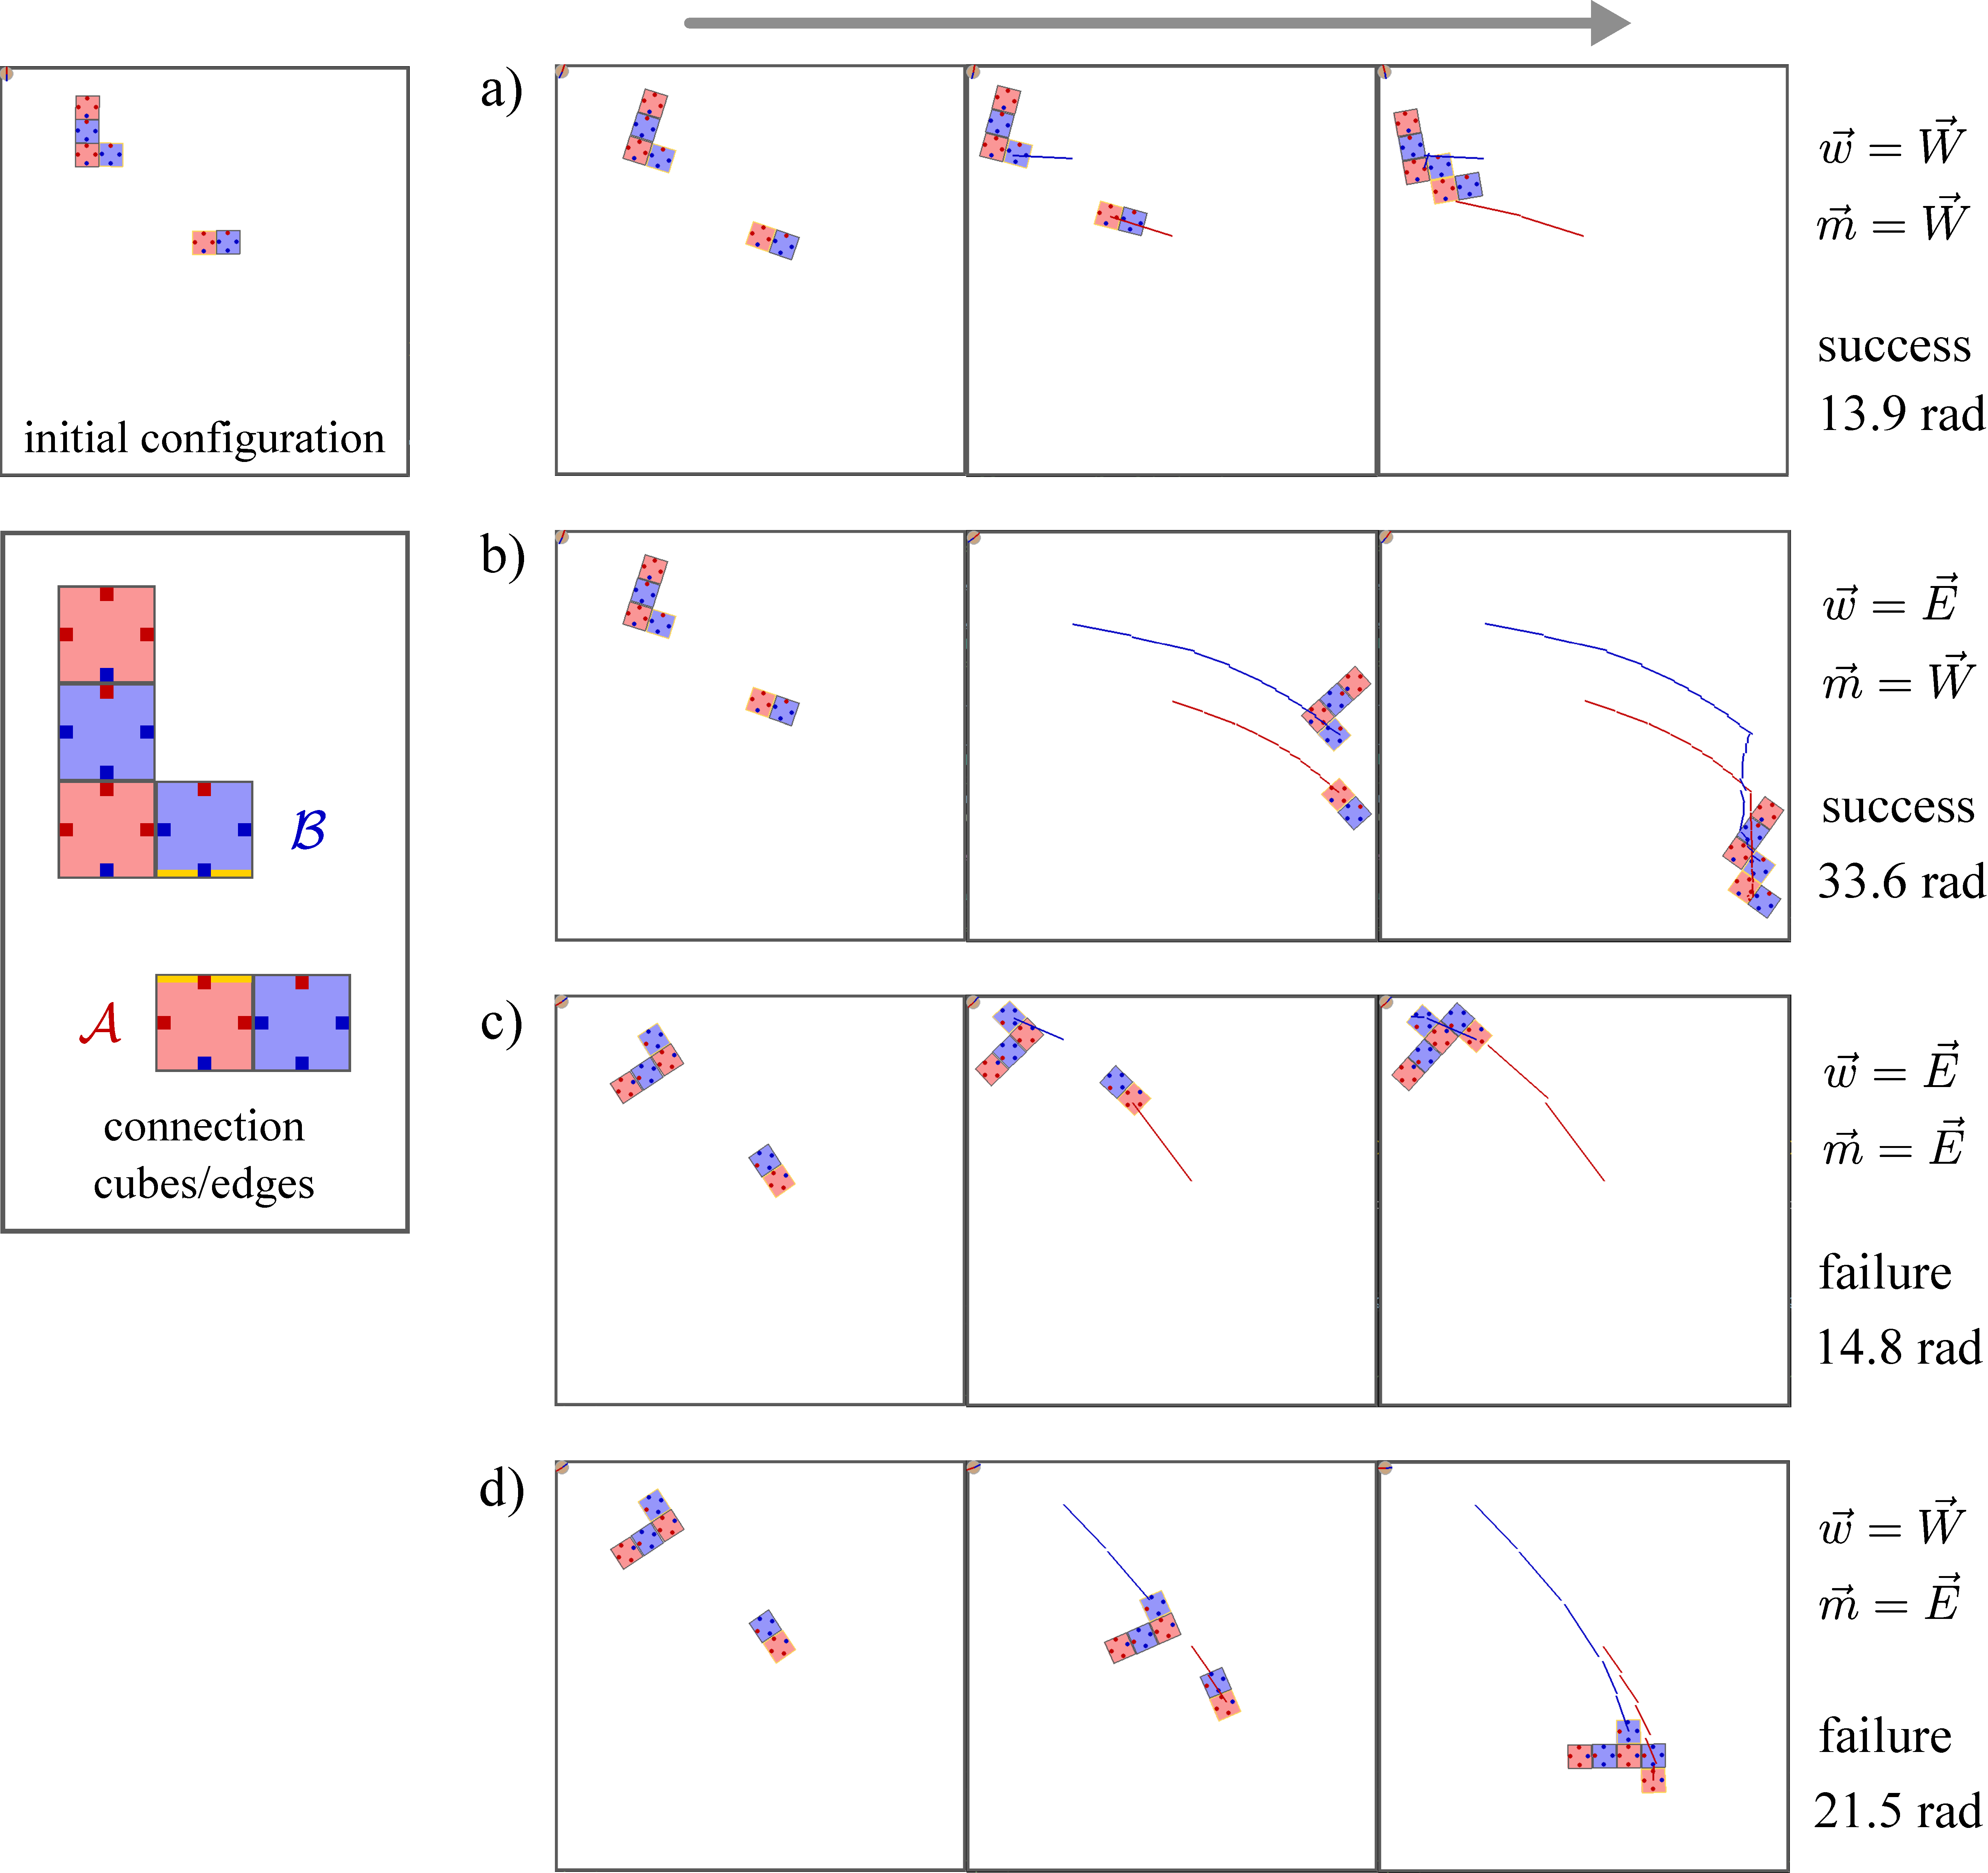
\includegraphics[width=1\textwidth]{figures/local_plans.pdf}
	\caption[Local plans for all pivot walking and slide-in directions]{Illustration of all local plans developed by \autoref{algo:local_algo} for different pivot walking direction $\vec{w}$ and slide-in directions $\vec{m}$. On the left side the initial configuration and connection cubes/edges of $\mathcal{A}$ and $\mathcal{B}$ are shown. Although both slide-in directions are possible, choosing $\vec{m}=\vec{E}$ results in failure due to a wrong connection for both c) and d). The two successful plans a) and b) have a huge difference in plan cost. a) would be the cheaper plan returned by the local planner. In b) $\mathcal{A}$ and $\mathcal{B}$ slide along the workspace boundaries until connecting in the bottom right corner. Both $c_\mathcal{A}$ (red) and $c_\mathcal{B}$ (blue) leave a trace when pivot walking.}
	\label{fig:local_plans}
\end{figure}

Before executing \autoref{algo:local_algo}, all failure conditions that can be pre-checked are evaluated, so no simulation-time is wasted on a plan that is bound to fail from the beginning.
While doing so, the possible slide-in directions are determined and \autoref{algo:local_algo} is executed with both pivot walking directions $\vec{w}$ for each possible $\vec{m}$.
This means two plans are developed for an east-west connection and two or four for a north-south connection, depending on the slide-in directions.
\autoref{fig:local_plans} shows an example of these four local plans created by \autoref{algo:local_algo}.

In the end, the successful plan with the lowest costs is returned.
If all plans fail, the best failure is determined.
Again, plans with lower costs are preferable, but we favor impossible connection and slide-in failures.
These failures just state that a specific connection cannot be established, but a global planner could continue to plan based on the goal configuration the local planner ended in.
A plan that ended due to polyominoes being stuck, or a reached maximum movement capacity, is not a good starting point for further planning.
Plans creating invalid polyominoes or polyominoes with caves will definitely be omitted on a global scale.

The different plans are developed in parallel and if one process finishes with a successful plan, the execution of all other processes can be canceled.
This saves computation time, although we might not return the best plan, since fastest computation does not automatically mean lowest costs.
Generally speaking a low computation time can be linked with low rotational cost, because the local planner spends the majority of time, about $98\%$, on simulating actions.

\paragraph{Align-Walk-Realign}

\autoref{algo:local_algo} takes the connection-cubes and edges $c_\mathcal{A}$, $c_\mathcal{B}$, $e_\mathcal{A}$, $e_\mathcal{B}$ along with $\vec{w}$, $\vec{m}$ and an initial configuration $g_\textit{init}$ as inputs and returns a plan-state $s$ along with the configuration $g_\textit{goal}$ the algorithm ended in after applying the sequence of actions $\mathcal{A}$.
The algorithm runs in a loop until $s$ changes to success or one of the failure condition.
The failure and success conditions are evaluated twice per iteration with {\scshape Update-State}.
This is done once after aligning and once at the end of the loop to avoid the simulation of unnecessary actions.
$g_\textit{goal}$ is updated by simulating the determined actions with {\scshape Simulate}.
The actions are appended to $A$ after simulation.
We perform either a straight or offset-align, depending on $e_\mathcal{A}$ and $e_\mathcal{B}$.
The offset-align is done with the direction of $\vec{m}$.
After aligning we walk the estimated amount of pivot walking cycles (\autoref{sec:walk_wait}) in direction $\vec{w}$ with {\scshape Walk}, or we wait with {\scshape Wait}, if $c_\mathcal{A}$ and $c_\mathcal{B}$ are in close proximity, determined by {\scshape Critical-Distance}.
If we waited in the previous iteration, we walk in the current one and oppositely.
This behavior is toggled by the variable ``wait''. 
The stuck condition is evaluated with {\scshape Stuck} and does not state failure immediately, since a straight-align might be able to fix the situation.
When the polyominoes are stuck, the algorithm performs a straight-align and waits as long as this changes the stuck condition.

\subsection{Complexity}
\label{sec:local_complex}

\paragraph{Optimality}

In our case the optimal plan for connecting two polyominoes is the one establishing the connection with the lowest rotational cost, defined in \autoref{sec:plan}.
We use this metric, because it is strongly linked with computation time, but can also be interpreted in a real word application of modular magnetic cubes.
Even if the local planner would not calculate plans in parallel, our dynamic approach of realigning does not produce optimal solutions.
It therefore simulates only the actions that are included in the final plan, which minimizes simulation time.

Optimality could be archived when sliding on walls and different polyomino displacements, as described in \autoref{sec:walk_wait}, are not existent.
In this hypothetical case both pivot walking directions produce plans that move the polyominoes together in a straight path.
The plan with the shorter path would be optimal.
In reality these factors have to be considered, and even if they were by a local planner in a pre-calculated way, it is hard to say if this is enough to prove optimality.

\paragraph{Completeness}

Our local planner is not complete.
We cannot exclude the existence of a solution just because the up to four dynamic plans developed fail.
If other polyominoes are blocking the way of $\mathcal{A}$ and $\mathcal{B}$, complex movements around these polyominoes, instead of the more or less straight path that we are taking, could create solutions where our local planner fails.
The reason we choose this simple an not complete approach is again to avoid simulation of movements as much as possible. 





	\chapter{Global Planner}
\label{chap:global}

The task of the global planner is to assemble a specified target polyomino $\mathcal{T}$ given an initial configuration $g_{init}$.
The configuration-space is explored by executing local plans developed by the local planner from \autoref{chap:local}.
That way, the part of the configuration-space we can actually explore is limited to configurations where a connection attempt between two cubes was made.
Compared to $SE(2)$ this part is manageable in size and only contains configurations which are relevant for self-assembly.

Determining how these configurations are explored affects the run time considerably.
Using rapidly-exploring random trees (RRTs) \cite{lavalle1998} yields good results in many cases, since the configuration-space gets evenly explored without the challenge of determining what decisions are promising for the end goal.
But it also explores many configurations which are not necessary for reaching the goal.
For us this approach is not reasonable. 
Because of the high fidelity simulation we are working with, the computation time for a local plan is huge, so planning the assembly of $\mathcal{T}$ with as few local plans as possible is the aim for our global planner.

We need to make well-thought-through connection decisions, that are valid for assembling $\mathcal{T}$, meaning some sort of building plan for a polyomino is needed.
Creating a building sequences by removing one tile at a time from the target was done by Becker et al.\ \cite{Becker2020}.
However, this does not consider sub-assemblies, so all cubes that are not to be connected have to stay separated at any time.

It is hard to prevent sub-assemblies with magnetic cubes following the rules of tilt, so our approach uses an enumeration of ways to cut a polyomino into two parts (\autoref{sec:twocutting}), which will be used for generating a so-called two-cut-sub-assembly graph (\autoref{sec:tcsa}).
This graph functions as a building instruction along side the exploration of the configuration-space.
\autoref{sec:connect_options} provides a closer look on the use of the graph for decision making and \autoref{sec:local_in_global} explains the usage of the local planner on a global scale. 
Finally \autoref{sec:global_algo} combines previous techniques to a global planning algorithm.
For the algorithm the number of cubes in the workspace is limited to the size of $\mathcal{T}$.
An explanation on why is this done and why the problem becomes more complex when working with extra cubes, is provided in \autoref{sec:more_cubes}.


\section{Two-Cutting Polyominoes}
\label{sec:twocutting}

\begin{figure}
	\centering
	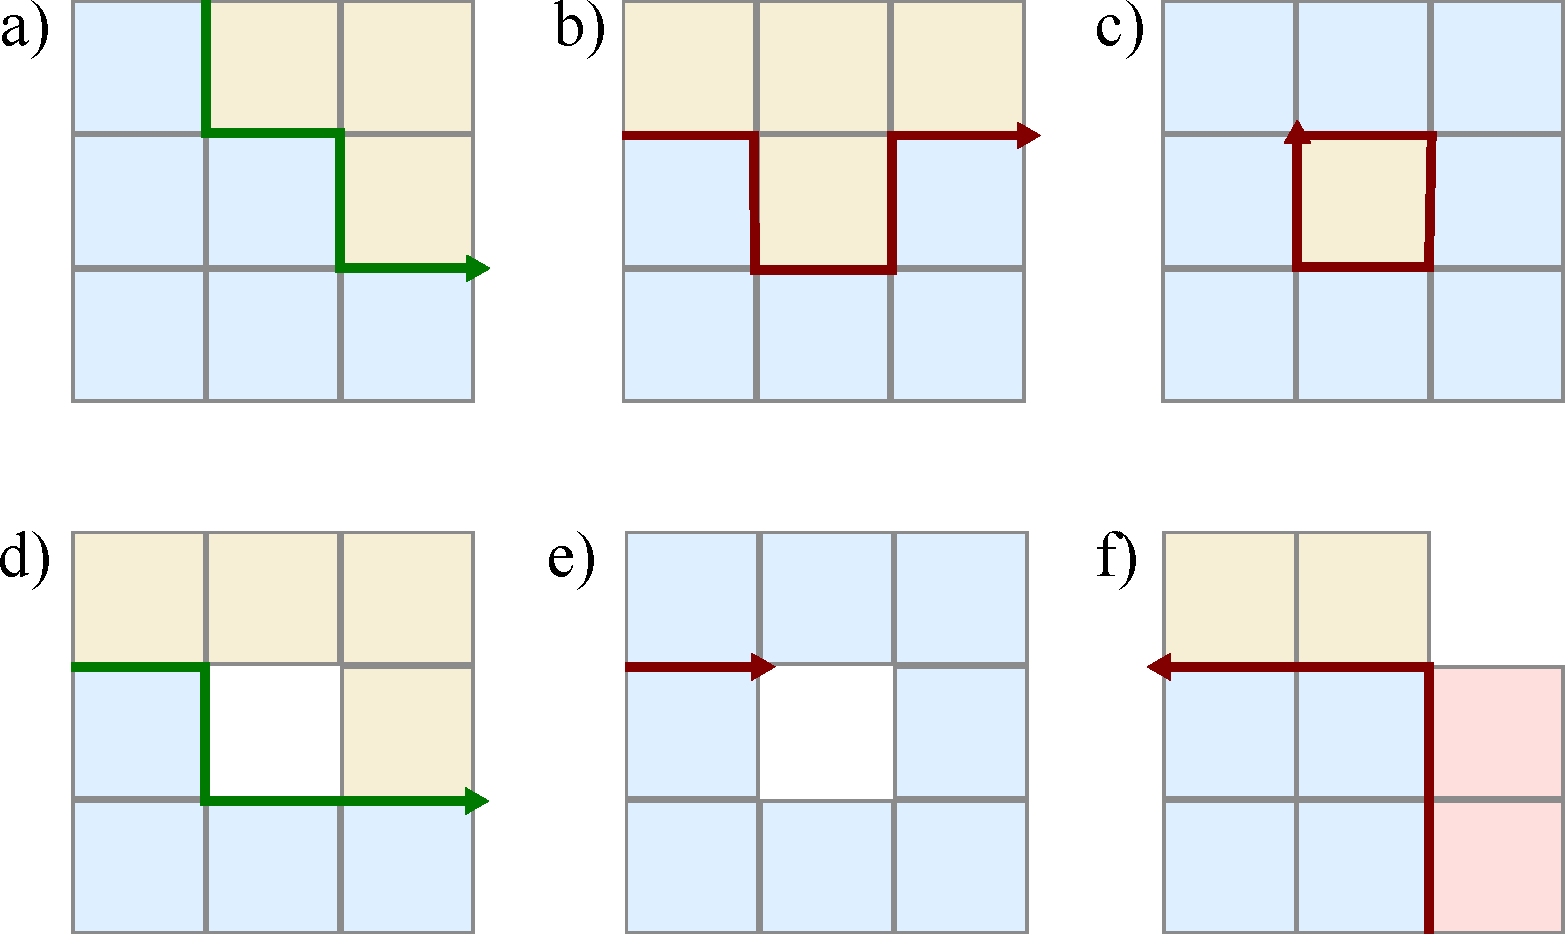
\includegraphics[width=0.6\textwidth]{figures/twocuts.pdf}
	\caption[Different cuts for polyomino shapes]{Examples for cutting polyomino shapes. a) to d) show three two-cuts for a $3\times3$ shape, of which only a) and d) are monotone and therefore valid. b) creates a cave and c) one a hole. e) and f) show cuts that do not split the polyomino into two pieces. e) does not break the polyomino at all and f) creates three sub-polyominoes.}
	\label{fig:twocuts}
\end{figure}

Schmidt et al.\ \cite{Schmidt2018} made use of straight-line two-cuts, to handle the construction of a polyomino with more than trivial sub-assemblies.

We define a two-cut as a continuous edge path through a polyomino that would divide the polyomino into two sub-polyominoes, if all connections with these edges are removed.
For later use in \autoref{sec:tcsa} we want to enumerate all two-cuts of a polyomino that are useful for planning.
We do not limit the cuts by only allowing straight paths like \cite{Schmidt2018}, instead we only consider monotone two-cuts.

\textit{Monotone} means that whenever the path goes into a direction it can never go into the opposite direction again.
\autoref{fig:twocuts} a) shows a monotone two-cut through a $3\times3$ polyomino shape.
The cut starts at the top of the shape and only moves down and right.
By removing all the connections on the path, the polyomino shape is split into two pieces.
Considering non-monotone two-cuts would create sub-assemblies with caves or holes, which could not be reassembled with our local planner.
For this reason they are omitted on a global scale in advance.
\autoref{fig:twocuts} b) shows a non-monotone two-cut creating a cave and \autoref{fig:twocuts} c) one creating a hole.

To calculate all two-cuts of a polyomino, we take all possible monotone paths from each connection as a starting point.
A path ends when it breaks out of the polyomino.
After the path ended the connection at its edges are removed from the polyomino and the path is added as a two-cut, if the polyomino got split into exactly two pieces.
\autoref{fig:twocuts} e) and f) show cuts that split the polyomino in less or more than two pieces.

% 32 possibilities for 3x3

\section{Two-Cut-Sub-Assembly Graph}
\label{sec:tcsa}

\begin{figure}
	\centering
	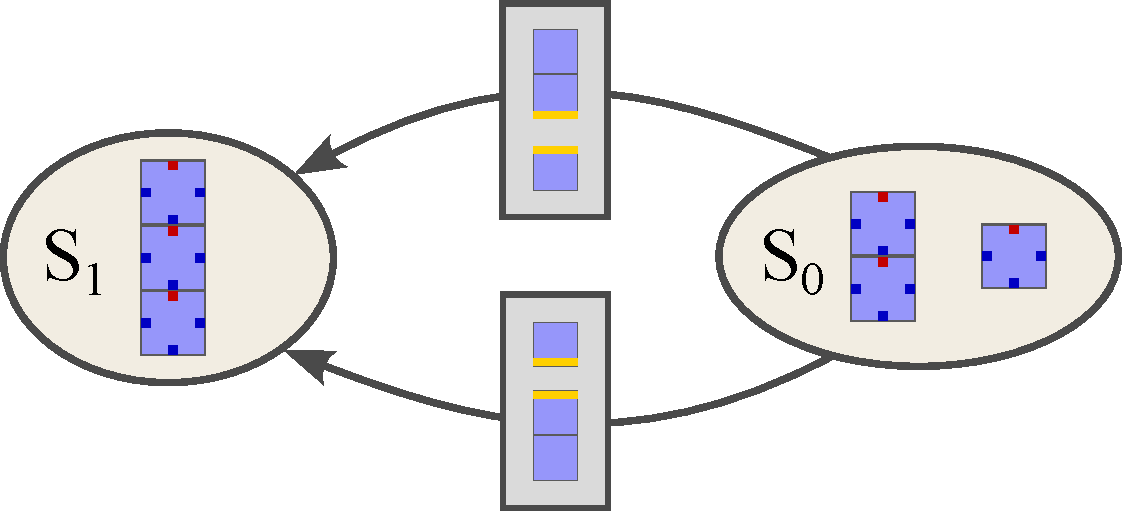
\includegraphics[width=0.45\textwidth]{figures/tcsa_multiedge.pdf}
	\caption[Two two-cut-sub-assembly nodes connected with multiple edges.]{Two two-cut-sub-assembly edges connecting the polyomino sets $S_0$ and $S_1$. The weights of the edges differ, since there are two ways to connect the $2\times1$ with the $1\times1$ to create a $3\times1$ polyomino. The connections are illustrated in rectangular boxes placed on the edges.}
	\label{fig:tcsa_multiedge}
\end{figure}

\begin{figure}
	\centering
	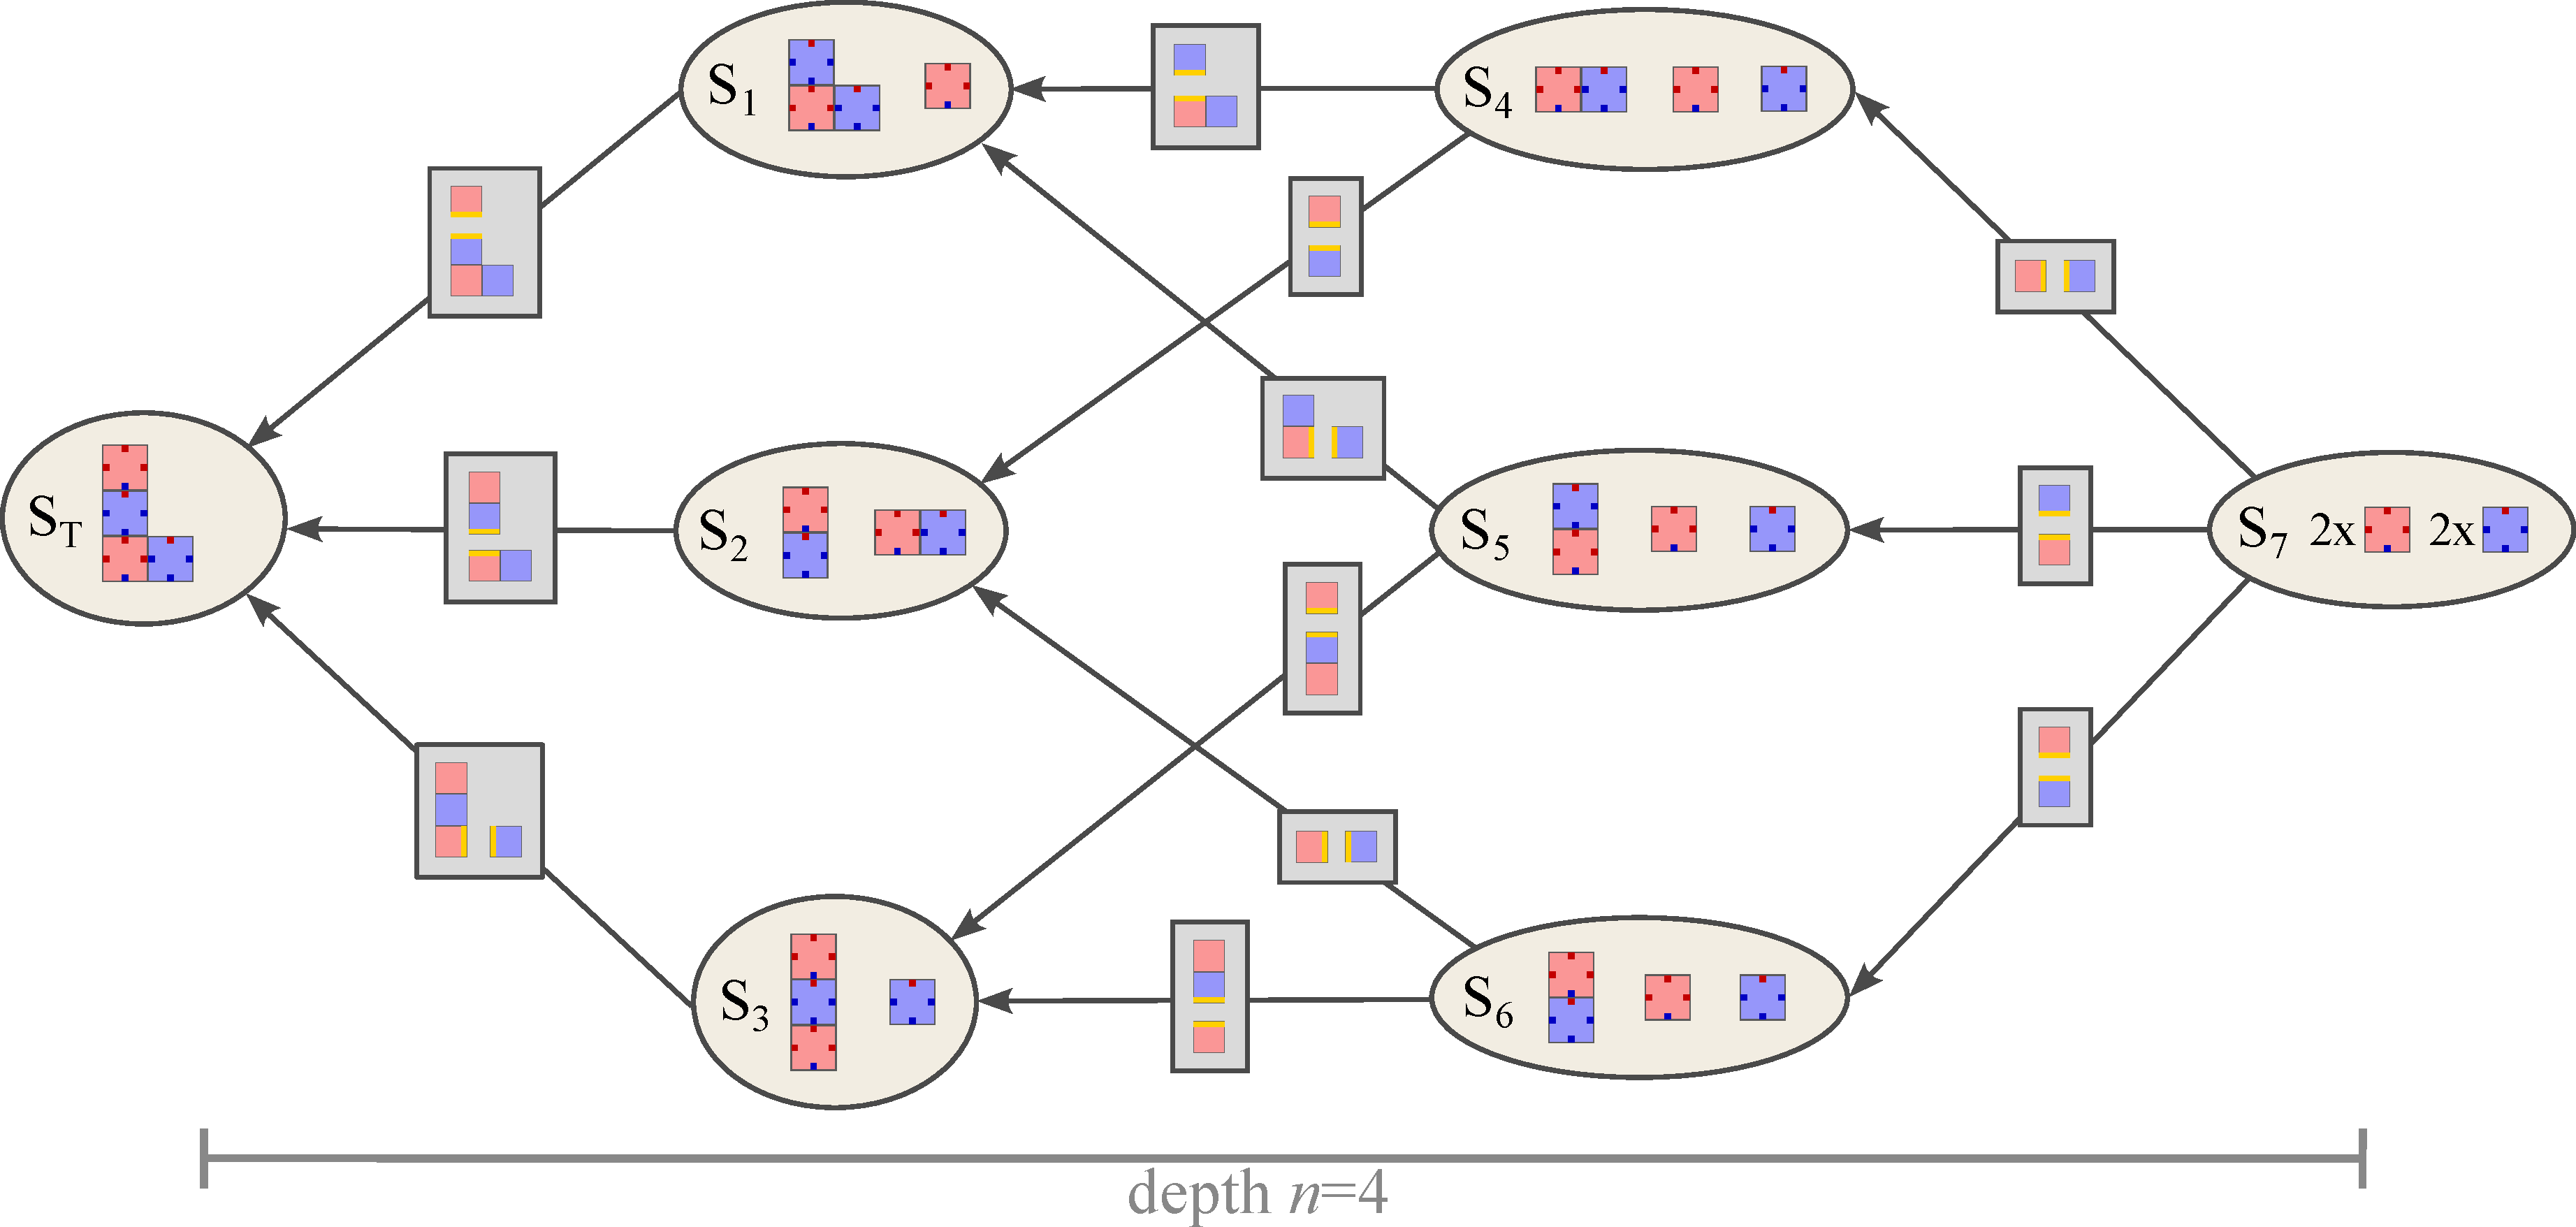
\includegraphics[width=1\textwidth]{figures/tcsa.pdf}
	\caption[Example for a two-cut-sub-assembly graph.]{Example of an two-cut-sub-assembly graph for a four-cube L-shape. The polyomino sets are illustrated as ellipses. If the polyominoes of a set are not numbered, there is only one occurrence of this polyomino. Otherwise the number of occurrences is placed left of the polyomino. The sets are numbered as if the graph was produced by \autoref{algo:build_tcsa} starting from $S_\mathcal{T}$. The weight of edges are illustrated as rectangular boxes containing the polyominoes that need to be connected at specific edges, marked in yellow.}
	\label{fig:tcsa}
\end{figure}

The two-cut-sub-assembly graph, short TCSA graph, functions as a building instruction for a specific target polyomino, we will call it $G_{\textit{TCSA}}(\mathcal{T})$.
The TCSA graph works with sets of polyominoes as nodes.
While a configuration $g$ holds information about orientation and position of physically distinct polyominoes, the corresponding polyomino set $S(g)$ only enumerates the polyomino types preset in $g$.
If $g$ contain multiple polyominoes of the same type, $S(g)$ still stores the amount of the polyomino type, but does not distinguish between the actual polyominoes.

Two nodes $S_0$ and $S_1$ of the TSCA graph are connected with an edge $\{S_0,w,S_1\}$, if $S_0$ can be transformed to $S_1$ by connecting two polyominoes contained in $S_0$.
The cube and edge information of the connections are stored as the weight $w$.
$S_0$ and $S_1$ can be connected by multiple edges, if there are different connections that produce the same outcome.
The edges differ in their weights as shown in \autoref{fig:tcsa_multiedge}.
The direction of $\{S_0,w,S_1\}$ always goes from $S_0$ to $S_1$, but we can reverse the definition for an edge as following:

Two nodes $S_0$ and $S_1$ are connected, if one polyomino contained in $S_1$ can be two-cut, so that the resulting polyomino set equals $S_0$.
This already provides a perspective on the use of two-cuts and the way $G_{\textit{TCSA}}(\mathcal{T})$ is built starting with $\mathcal{T}$.
We will further explain the building process along with an example of a TCSA graph provided in \autoref{fig:tcsa}.


\paragraph{Building a TCSA Graph}

\begin{algorithm}
	\caption{$\text{\scshape Build-TCSA-Graph}$}
	\label{algo:build_tcsa}
	\begin{algorithmic}[1]
		\REQUIRE $\mathcal{T}$ \COMMENT{target polyomino}
		\ENSURE $G_{\textit{TCSA}}(\mathcal{T})$ \COMMENT{the graph is represented by nodes $V$ and edges $E$} 
		\STATE $V \gets \{\}$
		\STATE $E \gets \{\}$
		\STATE $i \gets 0$
		\STATE $V[i] \gets S_\mathcal{T}$ \COMMENT{start with set only containing $\mathcal{T}$}
		\WHILE[work through nodes in BFS manner]{$i < \text{\scshape Size}(V)$}
			\STATE $S_i \gets V[i]$
			\FOR[go through all polyomino types in $S_i$]{\textbf{each} $\mathcal{A} \in S_i$}
				\FOR[go through all monotone two-cuts]{\textbf{each} $t_c \in \text{\scshape Two-Cuts}(\mathcal{A})$}
					\STATE $(\mathcal{A}_1, \mathcal{A}_2) \gets \text{\scshape Cut-Polyomino}(\mathcal{A}, t_c)$
					\STATE $S_{new} \gets \left( S_i \setminus \{\mathcal{A}\} \right) \cup \{\mathcal{A}_1, \mathcal{A}_2\}$ \COMMENT{new node after cutting}
					\IF{$S_{new} \notin V$}
						\STATE $V \gets \text{\scshape Append}(V, S_{new})$
					\ENDIF
					\STATE $E \gets \text{\scshape Append}(E, \{S_{new}, t_c, S_i\})$
				\ENDFOR
			\ENDFOR
			\STATE $i \gets i+1$
		\ENDWHILE
		\RETURN $(V,E)$
	\end{algorithmic}
\end{algorithm}

\autoref{algo:build_tcsa} describes the process of building $G_{\textit{TCSA}}(\mathcal{T})$ for the target $\mathcal{T}$.
The algorithm works through each newly added node in $V$ in a breadth-first-search manner.
The first node added to $V$ is $S_\mathcal{T}$, which is a polyomino set only containing the target shape.

New nodes and edges are determined by two-cutting every polyomino type $\mathcal{A}$ in the current set $S_i$ by every possible monotone two-cut of $\mathcal{A}$.
This is done by enumerating the two-cuts with {\scshape Two-Cuts}, the way it was described in \autoref{sec:twocutting}, and cutting $\mathcal{A}$ at the two-cut with {\scshape Cut-Polyomino}.
The cutting results in the two sub-polyominoes $\mathcal{A}_1$ and $\mathcal{A}_2$.
$S_{new}$ contains the same polyominoes as $S_i$ with the exception that one occurrence of $\mathcal{A}$ is removed and replaced by one occurrence of $\mathcal{A}_1$ and $\mathcal{A}_2$.
Each $S_{new}$ is the result of cutting one polyomino of $S_i$ at a specific two-cut $t_c$.
If $S_{new}$ is not already contained in $V$, we can add it to $V$, which also queues it for future iterations of the breadth-first-search.

No matter if $S_{new}$ is contained in $V$ or not, an edge going from $S_{new}$ to $S_i$ with $t_c$ as the weight is added to the graph edges $E$.
This allow multiple edges, as seen in \autoref{fig:tcsa_multiedge}, and multiple outgoing edges to different nodes, which can be observed in \autoref{fig:tcsa}, where different connections in $S_4$ lead to either $S_1$ or $S_2$.

Each two-cut applied to a polyomino set reduces its amount of polyominoes by one.
Let $n$ be the size of $\mathcal{T}$, then $n-1$ two-cuts applied to $S_\mathcal{T}$ will produce a polyomino set $S_{trivial}$ containing only trivial polyominoes, as it is the case for $S_7$ in \autoref{fig:tcsa}.
All $S_i$ will inevitably end up in this situation and the algorithm will return $(V,E)$, since trivial polyominoes cannot be cut anymore.
This means that no matter which connections are chosen along the way, $n-1$ edges will always be needed to get from $S_{trivial}$ to $S_\mathcal{T}$.
We describe this attribute, by giving the TCSA graph a depth of $n$.
The depth is also illustrated in \autoref{fig:tcsa} and the numbering of the nodes matches the order they were added by \autoref{algo:build_tcsa}.

\subsection{Complexity}

\begin{figure}
	\centering
	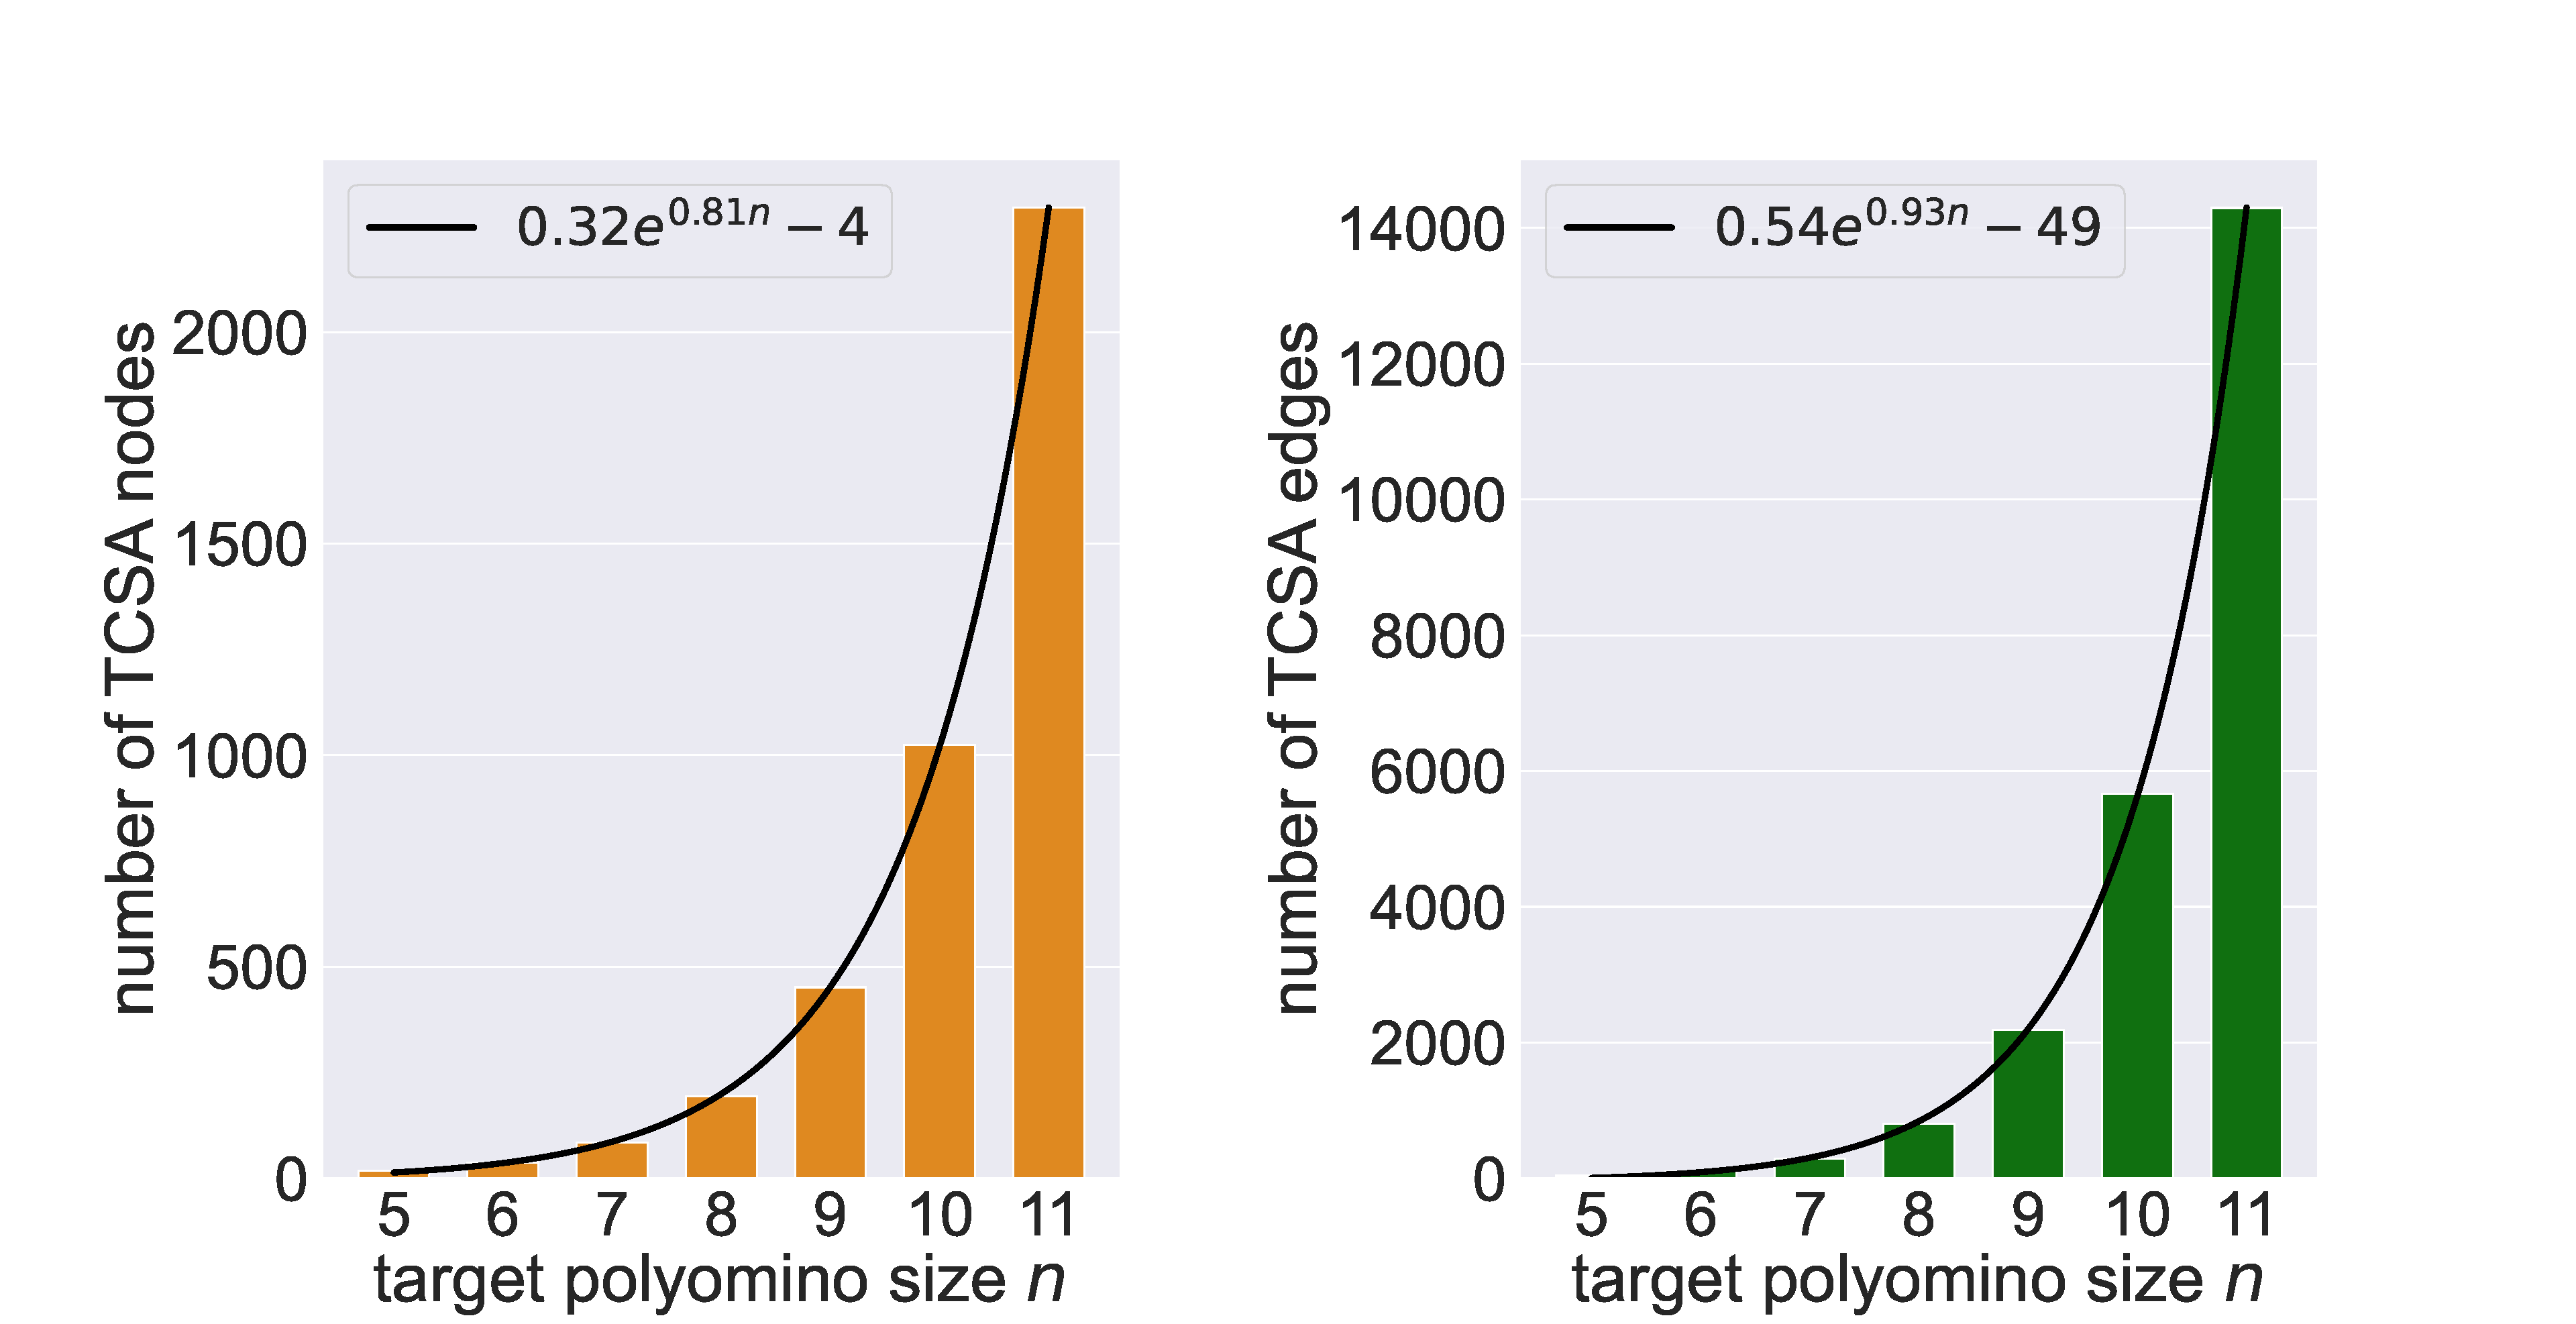
\includegraphics[width=0.8\textwidth]{figures/plots/tcsa_nodes_edges.pdf}
	\caption[Average two-cut-sub-assembly nodes and edges for target size $n$.]{Average number of nodes (left) and edges (right) of a TCSA graph for different target sizes $n$.
		For each target size $200$ samples of randomly generated polyominoes were taken.}
	\label{fig:tcsa_plot}
\end{figure}

The Stirling numbers of second kind provide an upper bound for the number of nodes in a TCSA graph.
The Stirling numbers of second kind
\begin{equation}
\bracenom{n}{k} = \sum_{i=1}^{k} \frac{(-1)^{k-i} \, i^{n-1}}{(i-1)! \, (k-1)!}
\end{equation}
describe the possibilities of sorting a set with $n$ objects into $k$ partitions \cite{jelliss1991}.
In our case $n$ equals the target size $n$ and the number of partitions $k$ is the number of polyominoes, the $n$ cubes belong to.
Different layers of depth account for different $\bracenom{n}{k}$.
$S_\mathcal{T}$ is the only polyomino set with $k=1$, so $\bracenom{n}{1} = 1$.
$S_{trival}$ is the only set containing $k=n$ polyominoes, so $\bracenom{n}{n} = 1$.
For the maximum number of nodes possible all layers of the TCSA graph have to be summed up
\begin{equation}
\#\textit{nodes}_\textit{worst} = \sum_{k=1}^{n} \bracenom{n}{k} \, ,
\end{equation}
which is also referred to as the Bell number \cite{jelliss1991}.

In our case, the only way of sorting cubes into partitions is by monotonously two-cutting existing polyominoes, which drastically lowers the number of $\#\textit{nodes}_\textit{worst}$.
In \autoref{fig:tcsa_plot} statistical data shows the average number of nodes and edges a TCSA graph consists of for varying target sizes $n$.
%TODO analyse grow trend. ie. exponenziell

Our implementation of $G_{\textit{TCSA}}(\mathcal{T})$ stores nodes in a hash-table.
Accessing nodes and connected edges, or checking if a polyomino set is contained in $G_{\textit{TCSA}}(\mathcal{T})$, can be done in  $\mathcal{O}(1)$.´
The creation of $G_{\textit{TCSA}}(\mathcal{T})$ becomes more complex for increasing numbers of $n$, but it provides an easily accessible building instruction that drastically cuts the number of unnecessary local plans simulated.
Lowering simulation time makes a complex data-structure like the TCSA graph worth the extra effort.


\section{Connection Options}
\label{sec:connect_options}

\begin{figure}
	\centering
	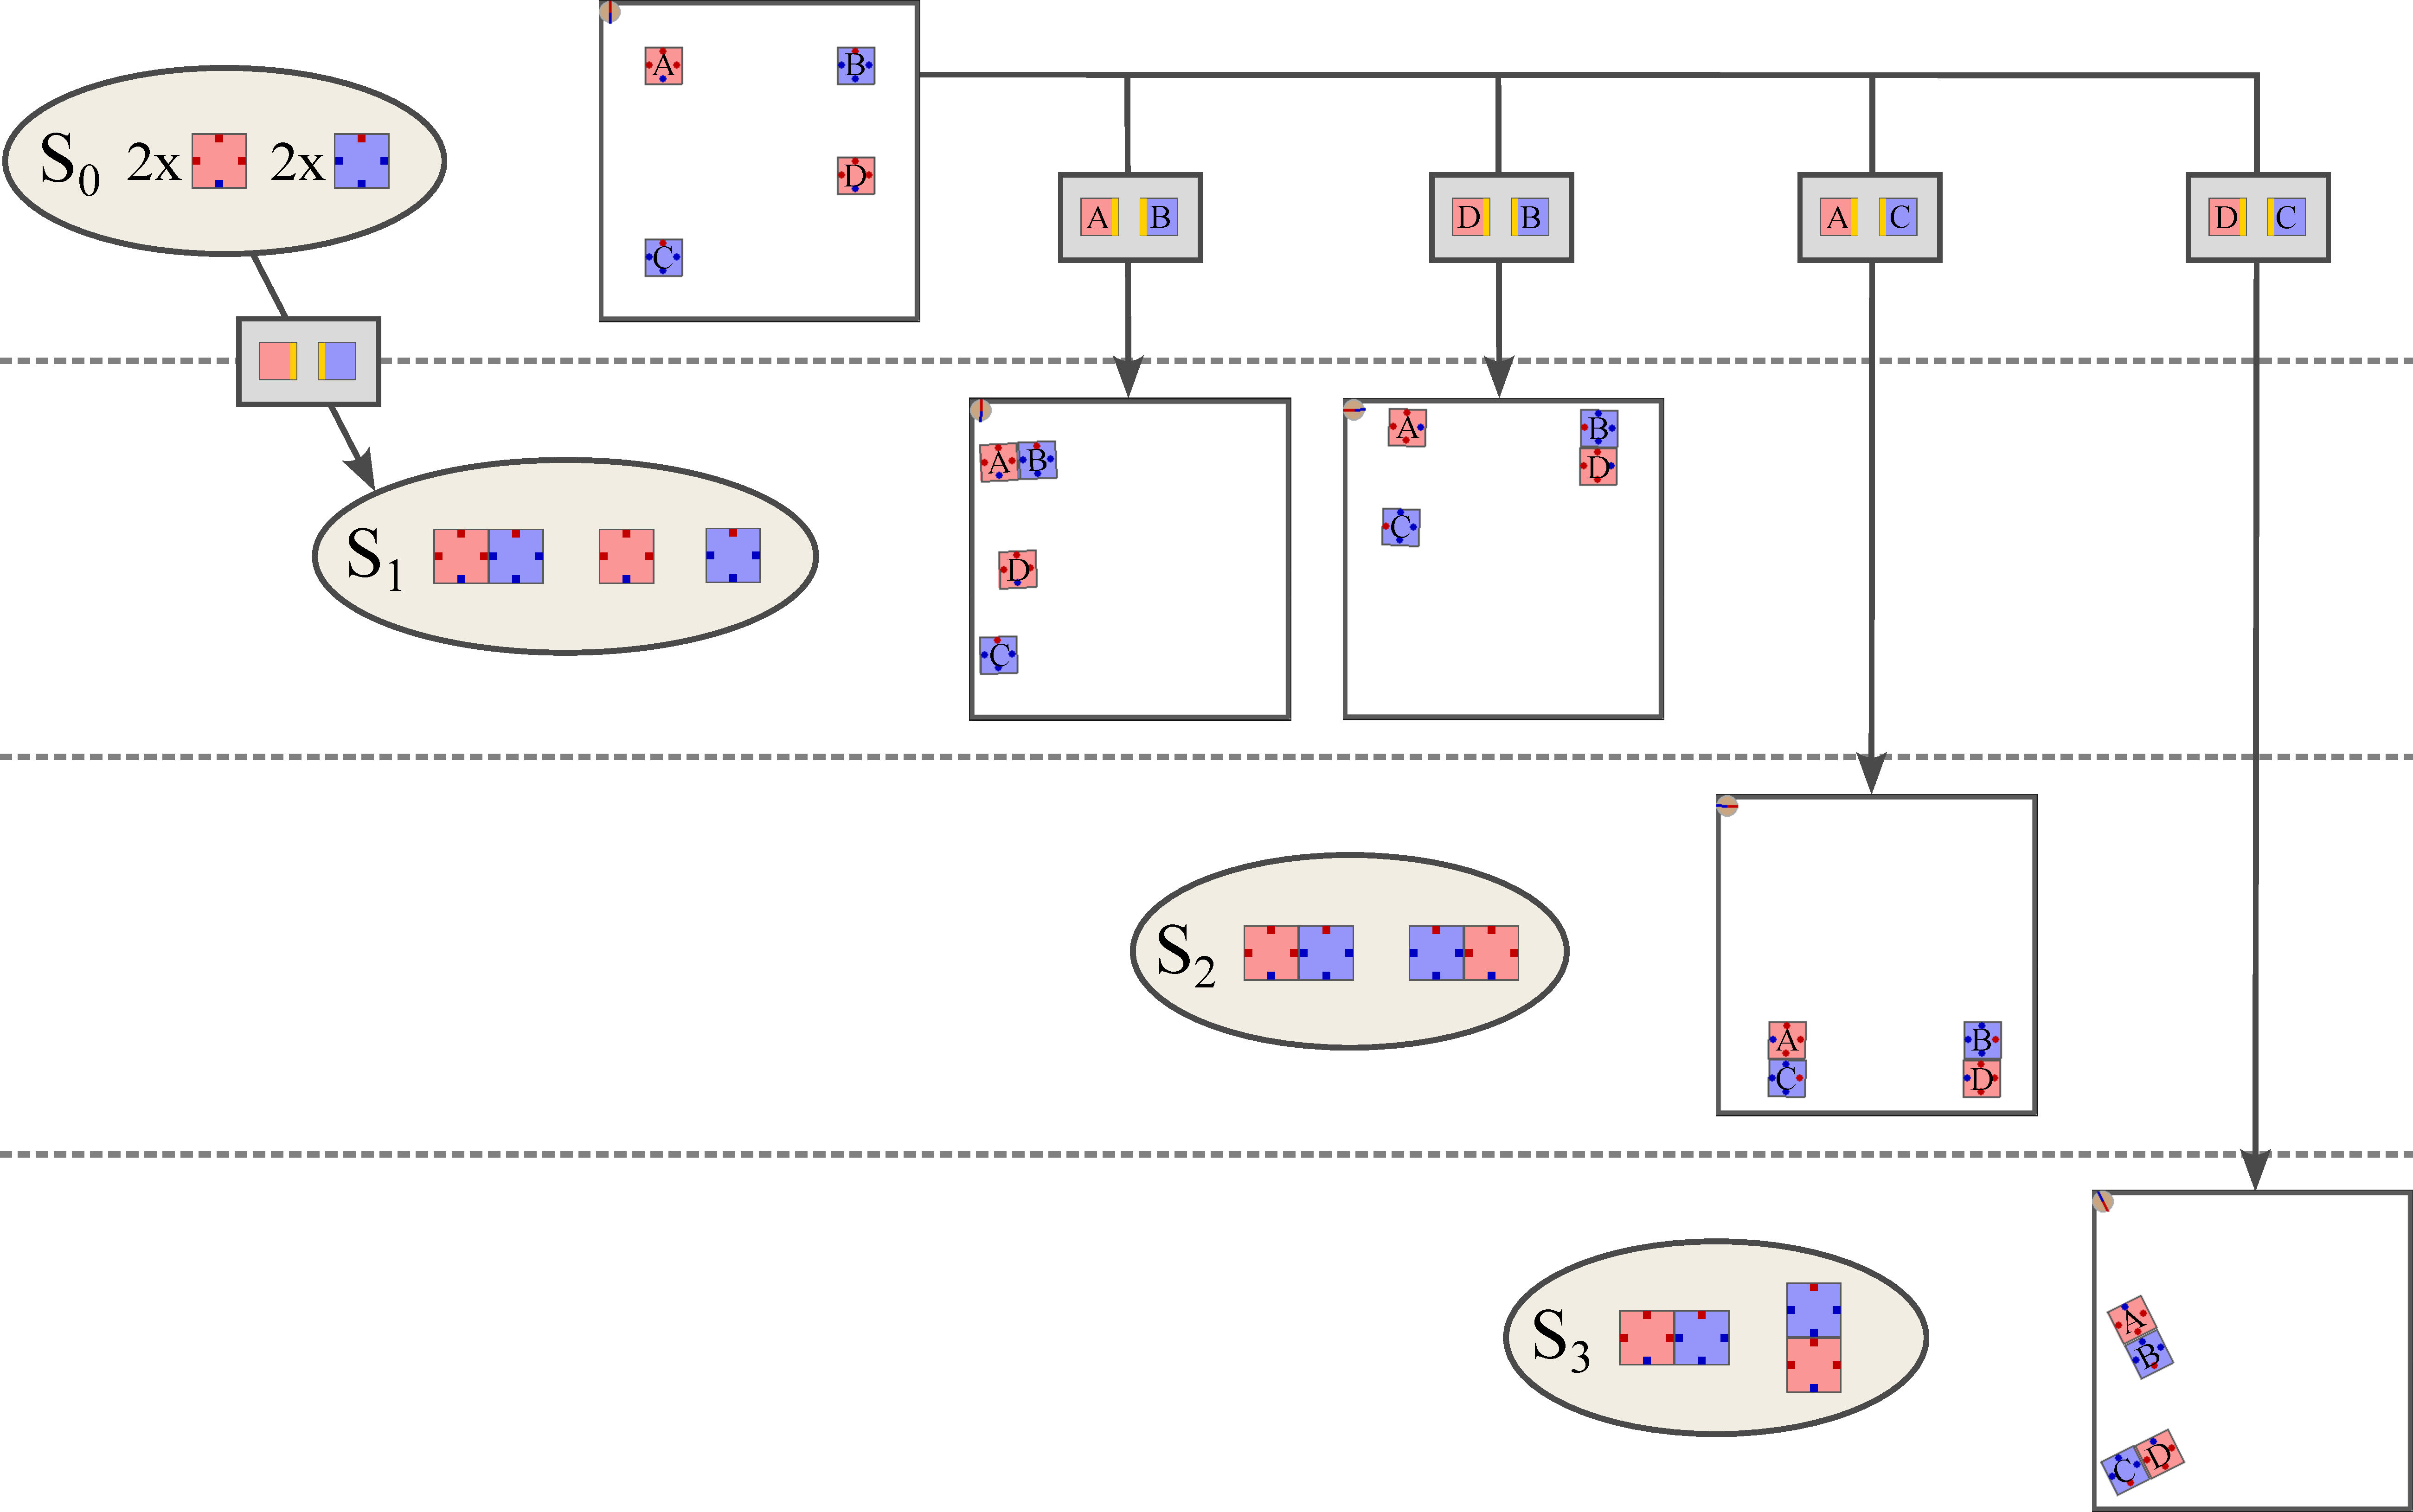
\includegraphics[width=1\textwidth]{figures/connect_options.pdf}
	\caption[Example of connection options for one two-cut-sub-assembly edge]{All connection options when connecting a red cube at the west of a blue cube to get from $S_7$ to $S_4$. Developing a local plan for different polyomino pairs, leads to different goal configurations. $(A_1,B_1)$ and $(A_2,B_1)$ lead to the desired polyomino set $S_4$, but $(A_2,B_2)$ leads directly to $S_2$. All these sets can be found in the TCSA graph of \autoref{fig:tcsa}. The goal configuration of $(A_1, B_2)$ holds the set $S_x$, which cannot be found in \autoref{fig:tcsa}. For further global planning this set could not be used.}
	\label{fig:connect_options}
\end{figure}

In each configuration $g$ the global planner encounters, $G_{\textit{TCSA}}(\mathcal{T})$ will be used to determine the next connection, that the local planner should try to establish.
$G_{\textit{TCSA}}(\mathcal{T})$ will be searched for the node that is the polyomino set $S(g)$.
If $S(g) \notin G_{\textit{TCSA}}(\mathcal{T})$, $g$ cannot be used to assemble $\mathcal{T}$.
This also allows the global planner to state failure immediately, when a initial configuration already contains sub-assemblies that are not usable for assembling $\mathcal{T}$.
With the exception of $S_\mathcal{T}$ all nodes have outgoing edges in a TCSA graph.
All outgoing edges of $S(g)$ provide connections for the local planner that bring the global planner closer to assembling $\mathcal{T}$.

For instance, if $S(g) = S_7$ in \autoref{fig:tcsa}, three outgoing edges provide three connections to choose from, but that is not all.
Assume the global planner decides to connect a red cube at the west edge of a blue cube to end up in a configuration $g_2$ with $S(g_2) = S_4$.
Since $S_7$ contains multiple polyominoes for the same type, there is more than one way to achieve this.
\autoref{fig:connect_options} illustrates all the different connection options for this example case.
You can also see how theses options differ in the goal configurations the local planner ended in.

Let $L_\mathcal{A}$ and $L_\mathcal{B}$ be collections of the physically distinct polyominoes for the polyomino types $\mathcal{A}$ and $\mathcal{B}$.
When $\mathcal{A}$ and $\mathcal{B}$ are about to be connected as the weight of a TCSA edge dictates, there are $\left| L_\mathcal{A} \times L_\mathcal{B} \right|$ polyomino pairs to choose from.
If $\mathcal{A} = \mathcal{B}$, the options where a polyomino will be connected with itself can be eliminated.

With multiple edges and various polyomino pairs per edge, many options emerge for the global planner to consider.
We examined three sorting strategies for these options, to provide an order of the best probable outcome that the global planner can work through. 
The approaches are compared in \autoref{chap:results}.

\paragraph{Minimal Distance}

The minimal distance sorting sorts connection options based on the distance between the cubes that are about to be connected.
The idea is that a smaller distances requires less movement to connect, which means shorter simulation time and lower plan costs of the resulting plan.
Due to sliding on walls and different pivot walking distances, this is not true in every case, but it remains a good heuristic for sorting.
Less movement might even prevent unwanted sub-assemblies.

\paragraph{Grow Largest Component}

Another approach is to grow the largest component.
The options are sorted into classes of maximum polyomino sizes in the resulting polyomino sets.
We prefer TCSA edges that lead to sets containing the biggest polyominoes.
When the options for $S_4$ in \autoref{fig:tcsa} are sorted, the one leading to $S_1$ is preferred over the one leading to $S_2$, because $S_1$ contains a polyomino of size $3$, while $S_2$ only contains polyominoes of size $2$. 
The options within each class are sorted with the minimal distance approach.

If no other sub-assemblies occur, growing the largest component behaves like one-tile-at-a-time assembly.
The benefit is, that even if they occur the TSCA graph can provide solutions to integrate them if possible.
Larger polyominoes generally move faster acting positive on plan costs.

\paragraph{Grow Smallest Component}

Oppositely to growing the largest component, options can be sorted by the smallest maximum size of polyominoes in polyomino sets.
This avoids working with large polyominoes, which are faster, but also need more simulation time to perform rotations and can be hard to handle, because of sheer size.

%TODO equations formel fall unterscheidung 

\section{Use of Local Planner}
\label{sec:local_in_global}

The local planner develops plans for connections chosen from the different connection options presented in \autoref{sec:connect_options}.
For the local planner only one connection, out of the path of connections stored in the weight of a TSCA edge, needs to be picked.
Whenever a path consists of both north-south and east-west connections, a north-south connection is preferred.
This is done to perform offset-aligning instead of straight-aligning (\autoref{sec:align}), for an easier slide-in.
Besides of that, the choice of connection is irrelevant, since all connections in the path lead to the same outcome.

When the local planner successfully connects the desired polyominoes, other sub-assemblies can lead to a different polyomino set than expected.
This is not necessarily bad, as long as the resulting set is contained in $G_{\textit{TCSA}}(\mathcal{T})$.
In-fact, more sub-assemblies decrease the number of polyominoes in the workspace, which brings the goal of assembling $\mathcal{T}$ even closer.
Layers of depth were skipped in the TCSA graph, so that it might be possible to assemble $\mathcal{T}$ with less than $n-1$ local plans.
This can be seen in \autoref{fig:connect_options}, where $A_2$ and $B_2$ were connected. 
The resulting polyomino set matches with $S_2$ instead of $S_4$ of the nodes from \autoref{fig:tcsa}.

Like already mentioned in \autoref{sec:connect_options}, when the resulting polyomino set is not in $G_{\textit{TCSA}}(\mathcal{T})$, it is not possible to assemble the target from that configuration.
This can be seen in \autoref{fig:connect_options} when connecting $A_1$ and $B_2$.
For global use we add a new failure condition to the local planner, which checks if the polyomino set of the configuration in the workspace is contained in $G_{\textit{TCSA}}(\mathcal{T})$.
If not, the planner immediately states failure and avoids spending simulation time on a configuration with no further use.

The local planner might even fail to establish the desired connection.
If the resulting polyomino set is contained in $G_{\textit{TCSA}}(\mathcal{T})$, global planning can continue, but there are certain failure types that are not valid for further planning.
Polyomino sets with invalid polyominoes, or where connections in caves are necessary, should not be present in the TCSA graph anyway, but we also do not continue planning with a failure due to maximum movement capacity or polyominoes being stuck.

\section{Global Planning Algorithm}
\label{sec:global_algo}

\begin{algorithm}
	\caption{\scshape Assemble-Target}
	\label{algo:global_algo}
	\begin{algorithmic}[1]
		\REQUIRE $\mathcal{T}$, $g_{init}$ \COMMENT{target polyomino and intital configuration}
		\ENSURE $s$, $P$ \COMMENT{state of global plan $s$ and plan stack $P$ containing local plans}
		\STATE $G_{\textit{TCSA}}(\mathcal{T}) \gets \text{\scshape Build-TCSA-Graph}(\mathcal{T})$
		\STATE $s \gets \text{undefined}$
		\STATE $P \gets \{\}$ 
		\STATE $g \gets g_{init}$ \COMMENT{current configuration $g$}
		\LOOP
			\STATE $O \gets \text{\scshape Connection-Options}(g, G_{\textit{TCSA}}(\mathcal{T}))$
			\STATE valid $\gets$ \FALSE
			\WHILE[try options until local plan is valid]{\NOT $\text{\scshape Empty}(O)$ \AND \NOT valid}
				\STATE $(c_\mathcal{A}, c_\mathcal{B}, e_\mathcal{A}, e_\mathcal{B}) \gets \text{\scshape Pop}(O)$
				\STATE $p_{new} \gets \text{\scshape Local-Planner}(g, (c_\mathcal{A}, c_\mathcal{B}, e_\mathcal{A}, e_\mathcal{B}), G_{\textit{TCSA}}(\mathcal{T}))$
				\IF{$\text{\scshape Valid-Plan}(p_{new})$}
					\STATE valid $\gets$ \TRUE
				\ENDIF
			\ENDWHILE
			\IF{valid}
				\STATE $P \gets \text{\scshape Push}(P, p_{new})$ \COMMENT{add new plan to plan stack}
				\STATE $g \gets g_{goal}$ of new local plan $p_{new}$ \COMMENT{move to new goal configuration}
				\IF[target got assembled]{$\mathcal{T} \in S(g)$}
					\STATE $s \gets \text{success}$
					\RETURN $(s, P)$
				\ENDIF
			\ELSE
				\IF[no configuration to fall back to]{$\text{\scshape Empty}(P)$}
					\STATE $s \gets \text{failure}$
					\RETURN $(s, P)$
				\ENDIF
				\STATE $p_{pre} \gets \text{\scshape Pop}(P)$ \COMMENT{remove last plan from plan stack}
				\STATE $g \gets g_{init}$ of last local plan $p_{pre}$ \COMMENT{fall back to last initial configuration}
			\ENDIF
		\ENDLOOP
	\end{algorithmic}
\end{algorithm}

The global planning algorithm provided in \autoref{algo:global_algo} takes the initial configuration $g_{init}$ and the target $\mathcal{T}$ as inputs and returns the state of the global plan $s$ and a plan stack $P$ as outputs.
For a successful plan, $P$ contains the local plans leading to the assembly of $\mathcal{T}$.
When concatenating the actions of all the plans in $P$, this creates a sequence of actions, that together form the global plan.
Because the local plans were created by using a TCSA graph, $|P| < n$ holds true (\autoref{sec:local_in_global}).
The reason for $P$ being called a stack is the way it is used in \autoref{algo:global_algo}.
The algorithm explores the configuration-space along $G_{\textit{TCSA}}(\mathcal{T})$ in a depth-first-search manner, which is done in the attempt to get closer to assembling $\mathcal{T}$ each iteration.

The algorithm starts with $g_{init}$ as the current configuration $g$.
At first all the connection options for $g$ are determined with {\scshape Connection-Options} the way it was described in \autoref{sec:connect_options}.
The mechanisem behind this function can be viewed as a hash-map, storing the options as the values for the configuration as the key.
The options need to be determined and sorted, only when it is the first time a configuration is encountered.
The list of connection options $O$ that {\scshape Connection-Options} provides, is only a view on the values stored in the hash-map, meaning that when $O$ is altered, the hash-map is updated as well.
Whenever a connection option is popped from $O$, this option is removed from the hash-map and will therefore never be considered again.
Note that options are stored per configuration $g$, not for the polyomino set $S(g)$.
Two configuration sharing the same polyomino set both have their own lists of connection options.
We traverse the configuration-space with the TCSA graph as a guidance, not the TCSA graph itself.
Nodes in $G_{\textit{TCSA}}(\mathcal{T})$ can be encountered multiple times and will never be eliminated from planning.

Once the list of connection options $O$ is retrieved, the algorithm works through it in the order determined by the option sorting that was applied in advance.
This is done until a valid local plan was found, or no options are left.
{\scshape Local-Planner} uses \autoref{algo:local_algo} to create a local plan $p_{new}$.
It also takes $G_{\textit{TCSA}}(\mathcal{T})$ as an input parameter, to ensure the newly added failure condition, when a configuration is not contained in $G_{\textit{TCSA}}(\mathcal{T})$.
The validity of a local plan is evaluated with {\scshape Valid-Plan}.

If a valid local plan was found, $p_{new}$ is pushed on to $P$ and $g$ is set to the goal configuration of $p_{new}$.
When a configuration containing $\mathcal{T}$ is reached, the global plan is successful and the algorithm returns.
On the other hand, if no valid option for $g$ could be found, the algorithm has to fall back to the last visited configuration.
For that the top local plan $p_{pre}$ on $P$ is popped and its initial configuration becomes the new $g$.
Even though $p_{pre}$ was a successful local plan, it led to a dead end and had to be removed from the stack.
If $P$ is empty the current configuration is $g_{init}$.
This means that there is no previously visited configuration the algorithm can fall back to.
In that case the algorithm has to state failure for assembling $\mathcal{T}$.

Before calling \autoref{algo:global_algo} one initial check for $S(g_{init})$ in $G_{\textit{TCSA}}(\mathcal{T})$ is necessary, to state early success.
Furthermore, a timeout failure is added to \autoref{algo:global_algo}, in case planning takes to long.
 
\subsection{Complexity}
\label{sec:global_complex}

\paragraph{Optimality}

Given that the local planner does not produce an optimal solution for the connection of two polyominoes, the global planner will also not reach optimality.
Even if the local planner provides only optimal solutions, our depth-first-search approach would not explore the configuration space in a way that the best sequence of local plans is guaranteed to be picked.
\autoref{algo:global_algo} greedily moves along the depth of the TCSA graph to assemble the target as fast as possible.
The option sorting strategies provide reasonable heuristics for picking a connection option per individual TCSA node, but cannot ensure the optimal decision, let alone the optimal decision for the whole path of connection options taken.
Optimal solutions would need broad exploration and comparison of different paths to the target, which is infeasible in our case due to the high simulation time required for local plans.

\paragraph{Completeness}

The same as with optimality, the local planner prevents the completeness of the global planner.
Assuming completeness of the local planner, the global planner could be certain of the existence or non-existence of a solution for assembling $\mathcal{T}$.
\autoref{algo:global_algo} will always return success or failure in finite time.
This is due to the finite number of connection options per configuration and the depth $n$ of the TCSA graph.
Each local plan in the plan stack is certain to connect at least two polyominoes, so after $n-1$ local plans the workspace contains only one $n$-size polyomino.
This polyomino is not necessarily $\mathcal{T}$, but no further connections can be made, which makes the algorithm fall back to the last configuration.
Together with the finite number of options per configuration, the algorithm will eventually explore all paths of connection options that are possible and can therefore verify the existence or non existence of a solution.
Remember that this completeness is based purely on the strong assumption of a complete local planer, which is challenging to archive in the special Euclidean group.

\paragraph{Efficiency}

We have to differentiate between local plans in the plan stack and local plans created during planning $\#\textit{local}$.
Even though $|P| < n$, the global planner might have created more local plans, which were either invalid or had to be removed, because they lead to a dead end.
In a best case only one local plan could lead to the assembly of $\mathcal{T}$.
This is highly unrealistic, but theoretically possible, since layers of depth in the TCSA graph can be skipped.
A more realistic best case would be $n-1$ local plans created during planning. 
This would assume, that all local plans created were valid and lead directly to the target with no layer skipping.

In a worst case all paths of connection options have to be explored before stating failure.
In this worst case ``all'' means that each connection option at each configuration produces a valid local plan with no other sub-assemblies leading to a unique new configuration.
The only invalid local plans are the ones that lead to a configuration with one $n$-size polyomino that is not $\mathcal{T}$.
It is not possible to state the exact amount of worst case local plans, since the number of connection options per configuration varies.
By taking the average number of connection options per TCSA node $o_\mu$, we can define an estimate

\begin{equation}
\#\textit{local}_\textit{worst} = \sum_{i=1}^{n-1} {o_\mu}^i \, .
\end{equation} 
For $n = 10$ and $o_\mu = 20$ this results in $\#\textit{local}_\textit{worst} \approx 5 \cdot 10^{11}$.

It is impossible to simulate that many local plans in a reasonable time.
For that reason a timeout failure was added.
\autoref{chap:results} will provide experimental data on the number of $\#\textit{local}$ and what percentage of global plans time out.
The number of configurations explored $\#\textit{config}$ is also examined in the experiments to better portray the number of dead ends during planning.


%\subsection{Discretize Configurations}
% dont know if I wil actually implement, but talk about benefits or why not that neccessary


\section{More Cubes than Target}
\label{sec:more_cubes}

The number of cubes in the workspace is limited to the target size $n$ for the global planner to work.
The reason for this is linked with the use of TCSA graphs. 
Using a hash-table to find a TCSA node $S_{\textit{TCSA}}$ and check for equality with the configurations polyomino set $S(g)$ is simple and fast.
If a configuration holds more cubes then the TCSA nodes hold, we need to check if $S_{\textit{TCSA}} \subseteq S(g)$.
This cannot be done by hash comparing, so all nodes of the graph need to be checked, which would be very costly.
In addition to that, multiple nodes can be included in $S(g)$.
The global planner could handle this by summing up the connection options of all the nodes, but again this makes planning more complex and costly.

After assembling $\mathcal{T}$ all the leftover cubes could assemble various polyominoes.
We could enumerate all possible left over polyomino sets $S_l$ and remove all of them separately from $S(g)$ to check for $S_{\textit{TCSA}} = S(g) \setminus S_l$.
This would again result in multiple nodes and summed up connection options, but with the ability to hash compare for equality.
The number of $S_l$ can become huge for increasing numbers of leftover cubes leading to a less efficient global planner.





	\chapter{Simulator}
\label{chap:sim}

\begin{figure}
	\centering
	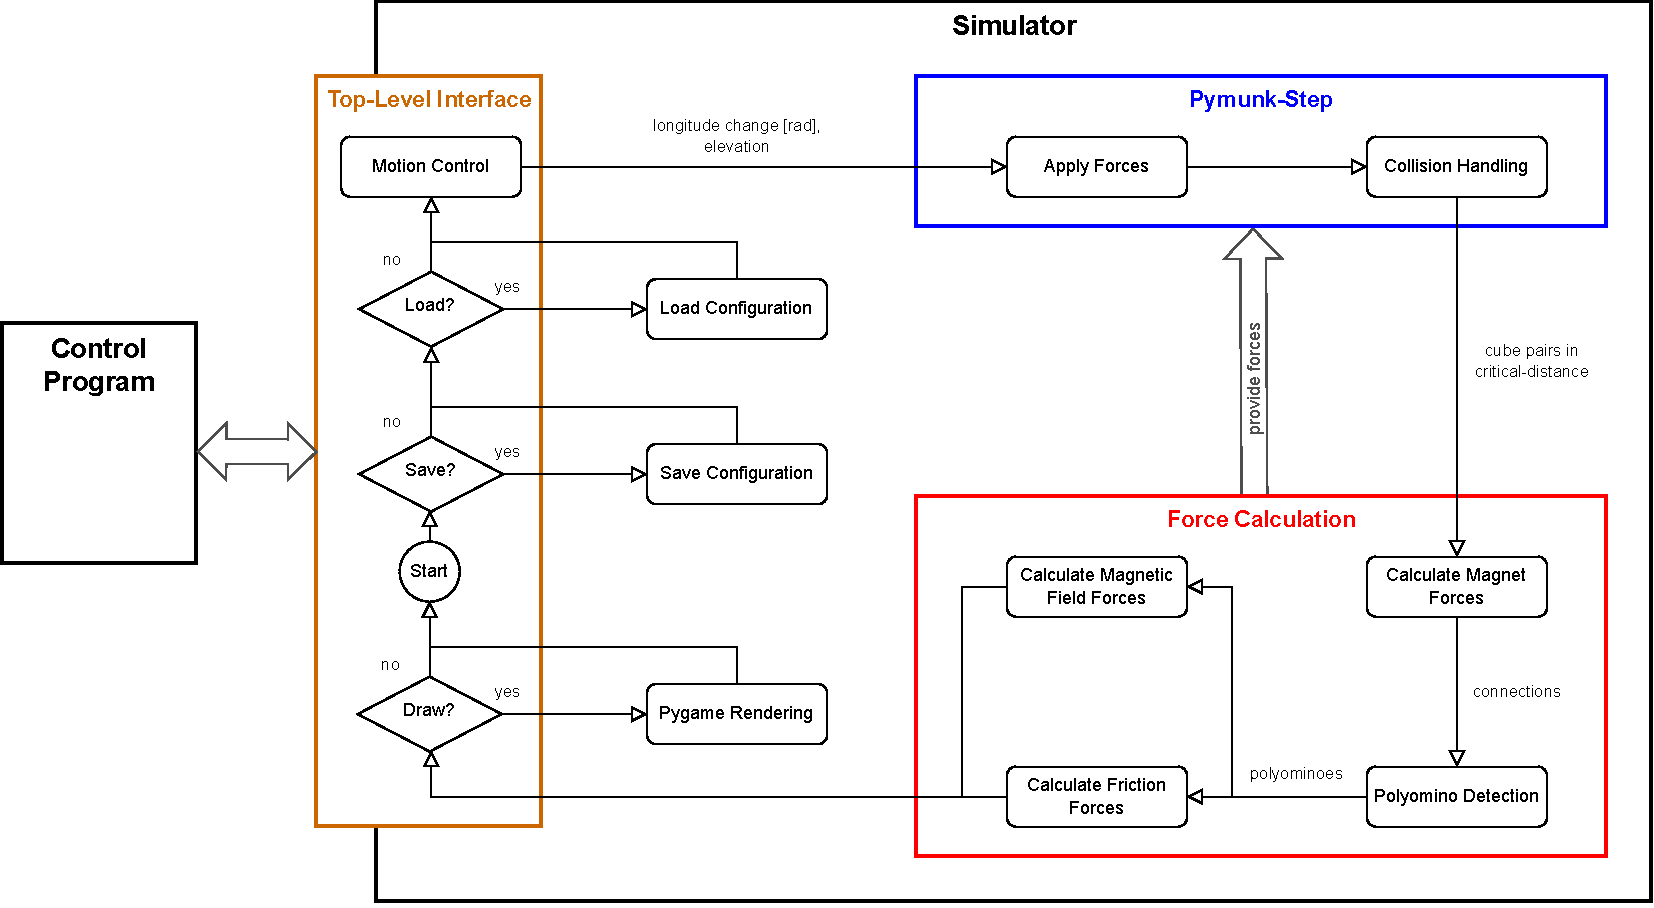
\includegraphics[width=1\textwidth]{figures/simulator_controlflow.pdf}
	\caption[Control flow of the simulator]{long caption...}
	\label{fig:simulator}
\end{figure}

Our simulator used for modeling the behavior of magnetic modular cubes uses the 2d physics library Pymunk\footnote{Pymunk: \url{https://www.pymunk.org/}}.
This library is build for the Python 3 and Python 2 environment based on the 2d physics library Chipmunk\footnote{Chipmunk: \url{http://chipmunk-physics.net/}}.
We used Pymunk, since it can be easily integrated and customized in a Python implementation.
Furthermore it is light-weight and capable of running headless, but also offers an interface for Pygame\footnote{Pygame: \url{https://www.pygame.org/}}, which we use to visualize developed plans and allowing user controls.
As a disadvantage, we are challenge with the simulation of 3d movement in a 2d environment.
That way we trade simulation accuracy for faster simulation time, which is necessary to develop global plans in a reasonable time.

\autoref{fig:simulator} shows a flow chart diagram of the simulators simulation loop.
The diagram provides the control flow of our simulator, where individual steps are explained in this and following sections.

Any control program, in example a local planner or a ``sandbox program'' for visually controlling magnetic modular cubes with keyboard inputs, can interact with the top-level interface of the simulator.
The interface provides functionalities like, starting and stopping the simulation process, controlling the drawing with Pygame, or loading custom configurations and retrieving the current workspace state (\autoref{sec:workspace_state}).
Another crucial functionality is queuing in motions for simulation and notifying the control program, when a motion is done simulating.
After handling the motion control, further explained in \autoref{sec:motion_control}, the simulator enters the Pymunk-step.

The Pymunk-step is a library function, responsible for updating the simulation environment by a certain time step.
The duration of a time step is a parameter that allows adjustment between simulation accuracy and simulation time. 
Inside the Pymunk-step forces are applied to the cubes and collision with workspace boundaries and between cubes is handled (\autoref{sec:coll_handling}).

After the Pymunk-step the magnetic forces between permanent magnets of cubes are calculated, which also determines connections of cube faces used to retrieve information about the polyominoes present in the workspace (\autoref{sec:force_magnet}).
Polyominoes are necessary to calculate the force of the magnetic field acting on cubes (\autoref{sec:force_field}) and friction forces, on which we heavily rely to simulate 3d movement like pivoting on pivot edges (\autoref{sec:force_friction}).
All the calculated forces will be applied in the Pymunk-step in the next iteration of the simulation loop.

When drawing is enabled the Pygame-rendering of the workspace is the last step before beginning the next iteration.

% plot of time use for simulation

\section{Motion Control}
\label{sec:motion_control}

The motion control manages the queued in motions from the control program and determines an update of the magnetic field for each iteration of the simulation loop.
This update consists of the longitude change in radians and the latitude change called the elevation.
In our simulator the elevation just states if the magnetic north points up, the magnetic south points up, or the magnetic field latitude lays in a neutral position within the workspace plane.
We do not specify a angular value of the latitude, since we cannot model it in the 2d-environment anyway.
The elevation just indicates the simulator to simulate pivoting of polyominoes.
More on that in \autoref{sec:force_friction}.

A change of elevation is executed in a single iteration, but the angle of a rotation will be simulated by multiple longitude changes in a linear ramp with a rotational velocity we choose to set to $\frac{\pi}{8} \, \text{rad}/\text{s}$.
Each motion will be simulated by applying its sequence of updates.
After that, the control program is notified to make closed loop control possible, by waiting until motions are done.

These updates control the magnetic field orientation and not magnetic modular cubes directly.
Cubes will orient themselves by magnetic field forces we further explain in \autoref{sec:force_field}.
The larger a polyomino is, the more time it needs to align with the magnetic field, which can take longer than rotating the magnetic field itself.
A certain amount of zero-updates is appended to a rotations update sequence depending on the size of the larges polyomino in the workspace.
That way the control program will not be notified until all polyominoes are aligned with the magnetic field.
For this reason simulating larger polyominoes requires more simulation time due to more iterations of the simulation loop.

\section{Workspace State}
\label{sec:workspace_state}

The state of the workspace is stored and updated within the Pymunk-space.
By saving a configuration of the workspace, relevant attributes like position, orientation and velocity of cubes are copied from the Pymunk-space.
These Pymunkt-space attributes will be manipulated when loading in a configuration.

Furthermore a configuration stores magnetic field orientation and the polyominoes, together with their center of mass and pivot points, that got detected by our polyomino detection method elaborated in \autoref{sec:force_magnet}.
Polyominoes are stored in a custom data structure that functions both as a list of physical polyominoes and a polyomino set for the use in two-cut-sub-assembly graphs (\autoref{sec:tcsa}).
The data structure and the polyominoes themselves are hashable for fast equality and inclusion checks.

Individual orientation and velocities of cubes will not be used for planning, but they ensure a correct loading of a workspace configuration that got saved while in motion or when cubes where not or not yet aligned with the magnetic field.
The alignment can be prevented by walls or other cubes, even though we assume perfect alignment with the magnetic field during planning.

\section{Collision Handling}
\label{sec:coll_handling}

Collision is detected and resolved by Pymunk during the Pymunk-step.
For the collision detection Pymunk uses a bounding volume hierarchy of objects in the Pymunk-space.
We also use this efficient collision detection for determining cube pairs in critical-distance.
For that, each cube is surrounded by a circular sensor with half the critical-distance as the radius.
Cubes are in critical-distance if two sensors collide.
Cubes not in critical-distance are to far away to significantly affect each other with magnetic forces of their permanent magnets.
We only calculate magnet forces for cube pairs in critical-distance to speed up simulation.
We set the critical-distance to be $5 r_C$.

\section{Simulating Forces}

% apply with pymunk

\subsection{Magnet Forces}
\label{sec:force_magnet}

% pull cubes together
% provide equation
% plot for magnetic attraction based on distance
% hold cubes together -> polyomino detection
% wich magnetic pairs to choose
% minDist, minDists, all

\subsection{Magnetic Field Forces}
\label{sec:force_field}

% applied to top bottom each indivial cube
% as long as orientation doenst match
% the bigger the poly the longer rotations actually take 
% adding zero updates to motion so that motion finishes when polys oriented


\subsection{Friction Forces}
\label{sec:force_friction}

% force to let poly rotate around pivot point
% splitt friction on cubes on pivot edge
% nominal friction to prevent breaking



	\chapter{Results}
\label{chap:results}

All experiments conducted are about assembling target polyominoes with the use of our global planner (\autoref{chap:global}).
In \autoref{sec:AFN} we analyze the effect of increasing polyomino size on planning time, rotational cost and other global planner characteristics mentioned in \autoref{sec:global_complex}.
The polyominoes used for this experiment are randomly generated, but we also evaluate the construction of manually designed polyominoes in \autoref{sec:AFTS}.
With manually designed polyominoes, we can specifically test the assembly of targets with caves or holes, varying widths and heights, or different patterns of red and blue cubes. 
Furthermore, we experiment with different workspace sizes and aspect ratios in \autoref{sec:AFBS} and how the ratio of red and blue cubes affect the assembly of straight line polyominoes in \autoref{sec:AFNR}.

\paragraph{Option Sorting Strategies}
We conducted all experiments with the three option sorting strategies from \autoref{sec:connect_options}:
\begin{enumerate}
	\item Minimal Distance (MIN DIST)
	\item Grow Largest Component (GROW LARGEST)
	\item Grow Smallest Component (GROW SMALLEST)
\end{enumerate}

\paragraph{Instance Generation}
Random polyominoes and initial configurations were created with a seed-based pseudorandom number generator, to make experiments reproducible.
The option sorting strategies are applied to the same set of seeds to make the results comparable.
When an initial configuration is randomly generated, the number of red and blue cubes matches with the target polyomino.
Sub-assemblies in the initial configuration can occur.

\paragraph{Timeout Failure}
The global planner states a timeout failure after a planning time of $600$ seconds.
We do not time out during the simulation of local plans, so instances can exceed $600$ seconds and still be successful if the last local plan assembles the target polyomino.

\paragraph{Hardware Setup}
The experiments were done on multiple computers with the same hardware specification (\textbf{AMD Ryzen 7 5800X @ 8x3.8 GHz (-4.7 GHz), 128 GB RAM}) running Ubuntu 22.04.2 LTS.

%TODO key legende fuer box-whisker plots




\section{Assembly for Polyomino Size}
\label{sec:AFN}

This experiment was conducted with randomly generated initial configuration and randomly generated polyominoes of specific size $n$.
To maximize the variety of possible polyomino shapes, the number of red cubes is set to $n_\textit{red} = \lfloor \frac{n}{2} \rfloor$ \cite{Lu2021}.
This makes the experiment well-suited for not only analyzing planning time and rotational-cost, but also examine $\#\textit{local}$, $\#\textit{config}$ and $|P|$.
The workspace is of size $50 r_C \times 50 r_C$ and for each target size $150$ samples were taken.

\paragraph{Planning Time}

\begin{figure}
	\centering
	\begin{subfigure}[b]{\textwidth}
		\centering
		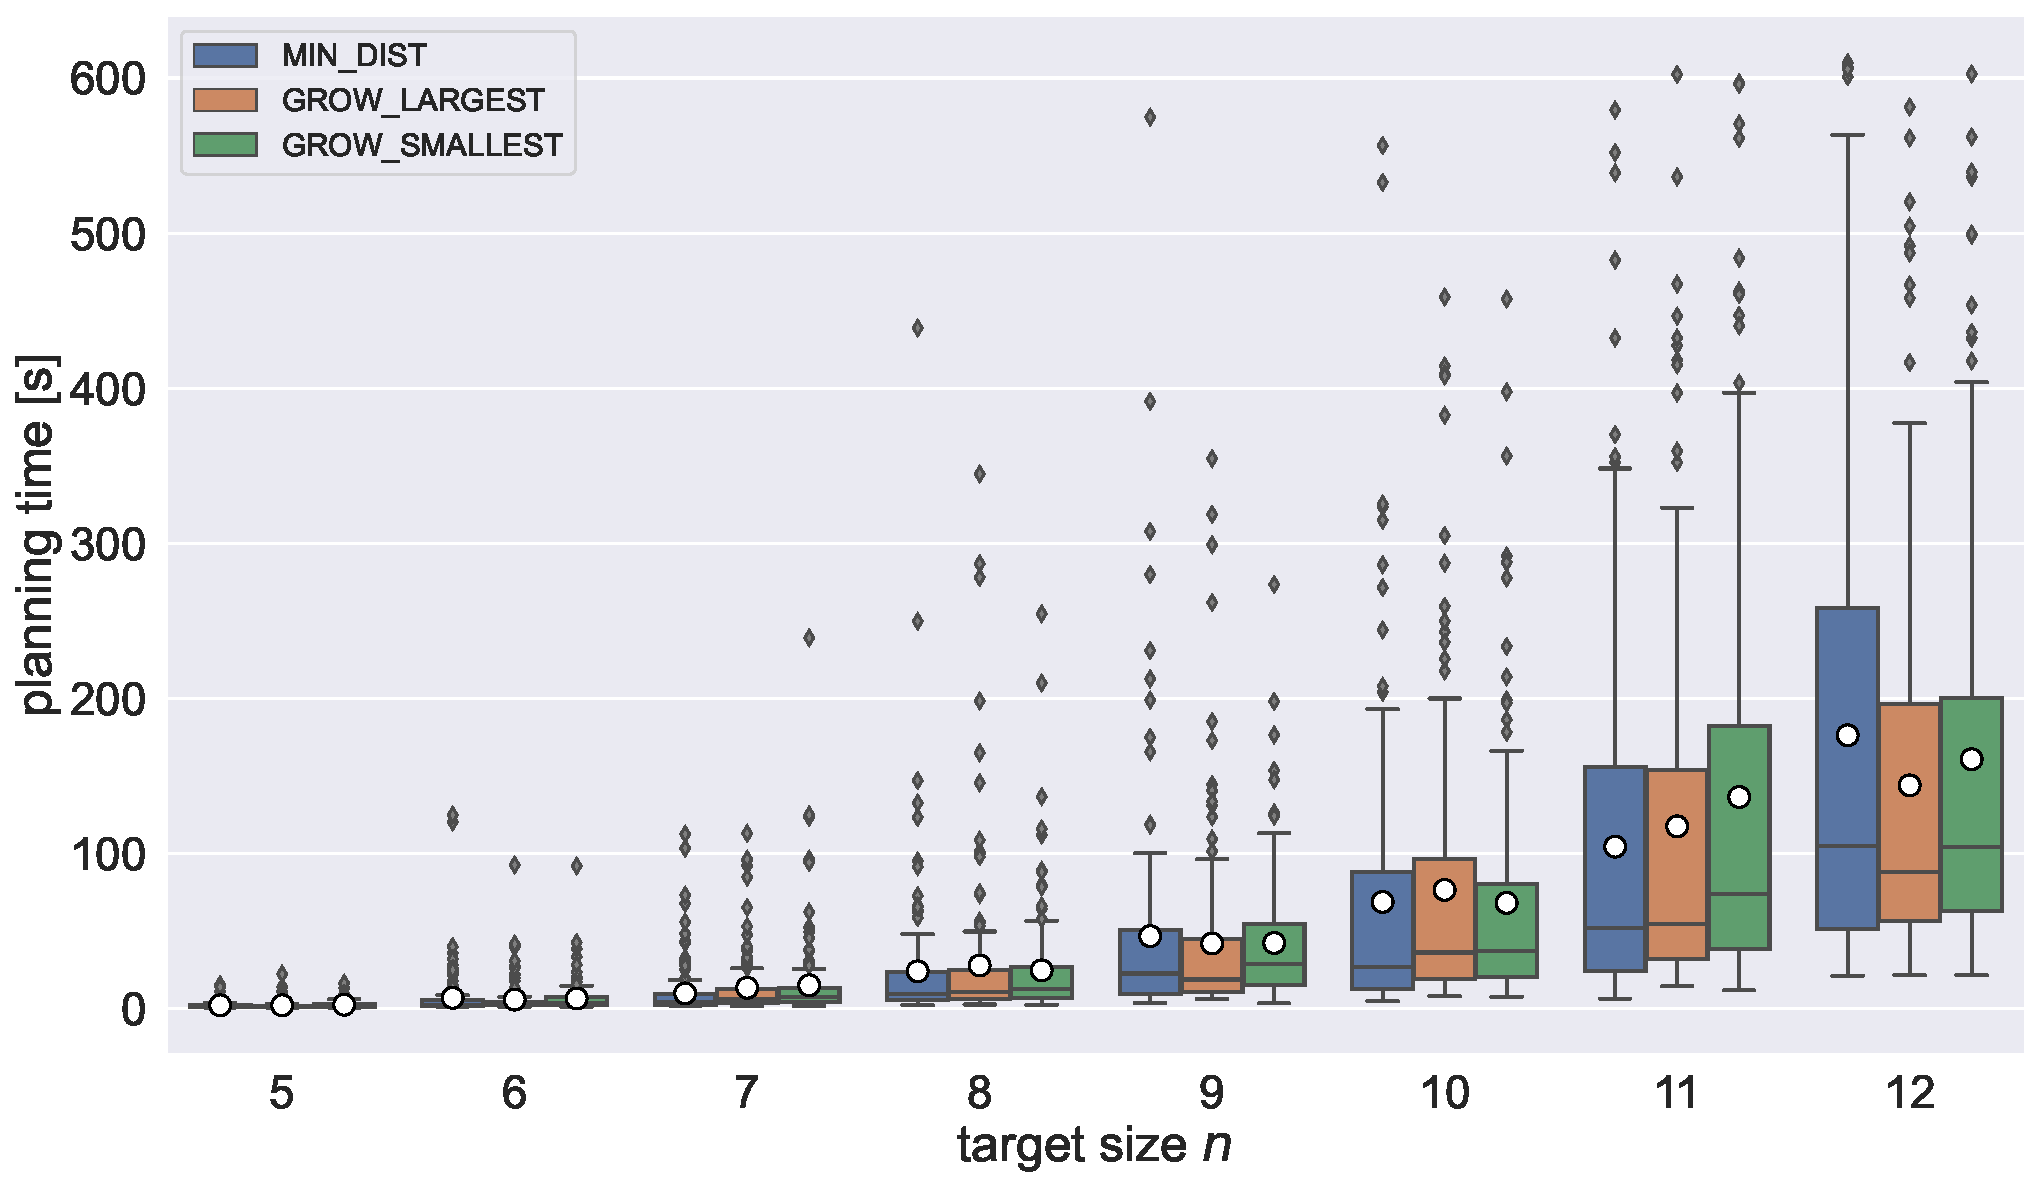
\includegraphics[width=0.9\textwidth]{figures/plots/AFN_time.pdf}
		\caption{Planning time in seconds. Only plans that did not time out are shown.}
		\label{fig:AFN_time}
	\end{subfigure}

	\begin{subfigure}[b]{\textwidth}
		\centering
		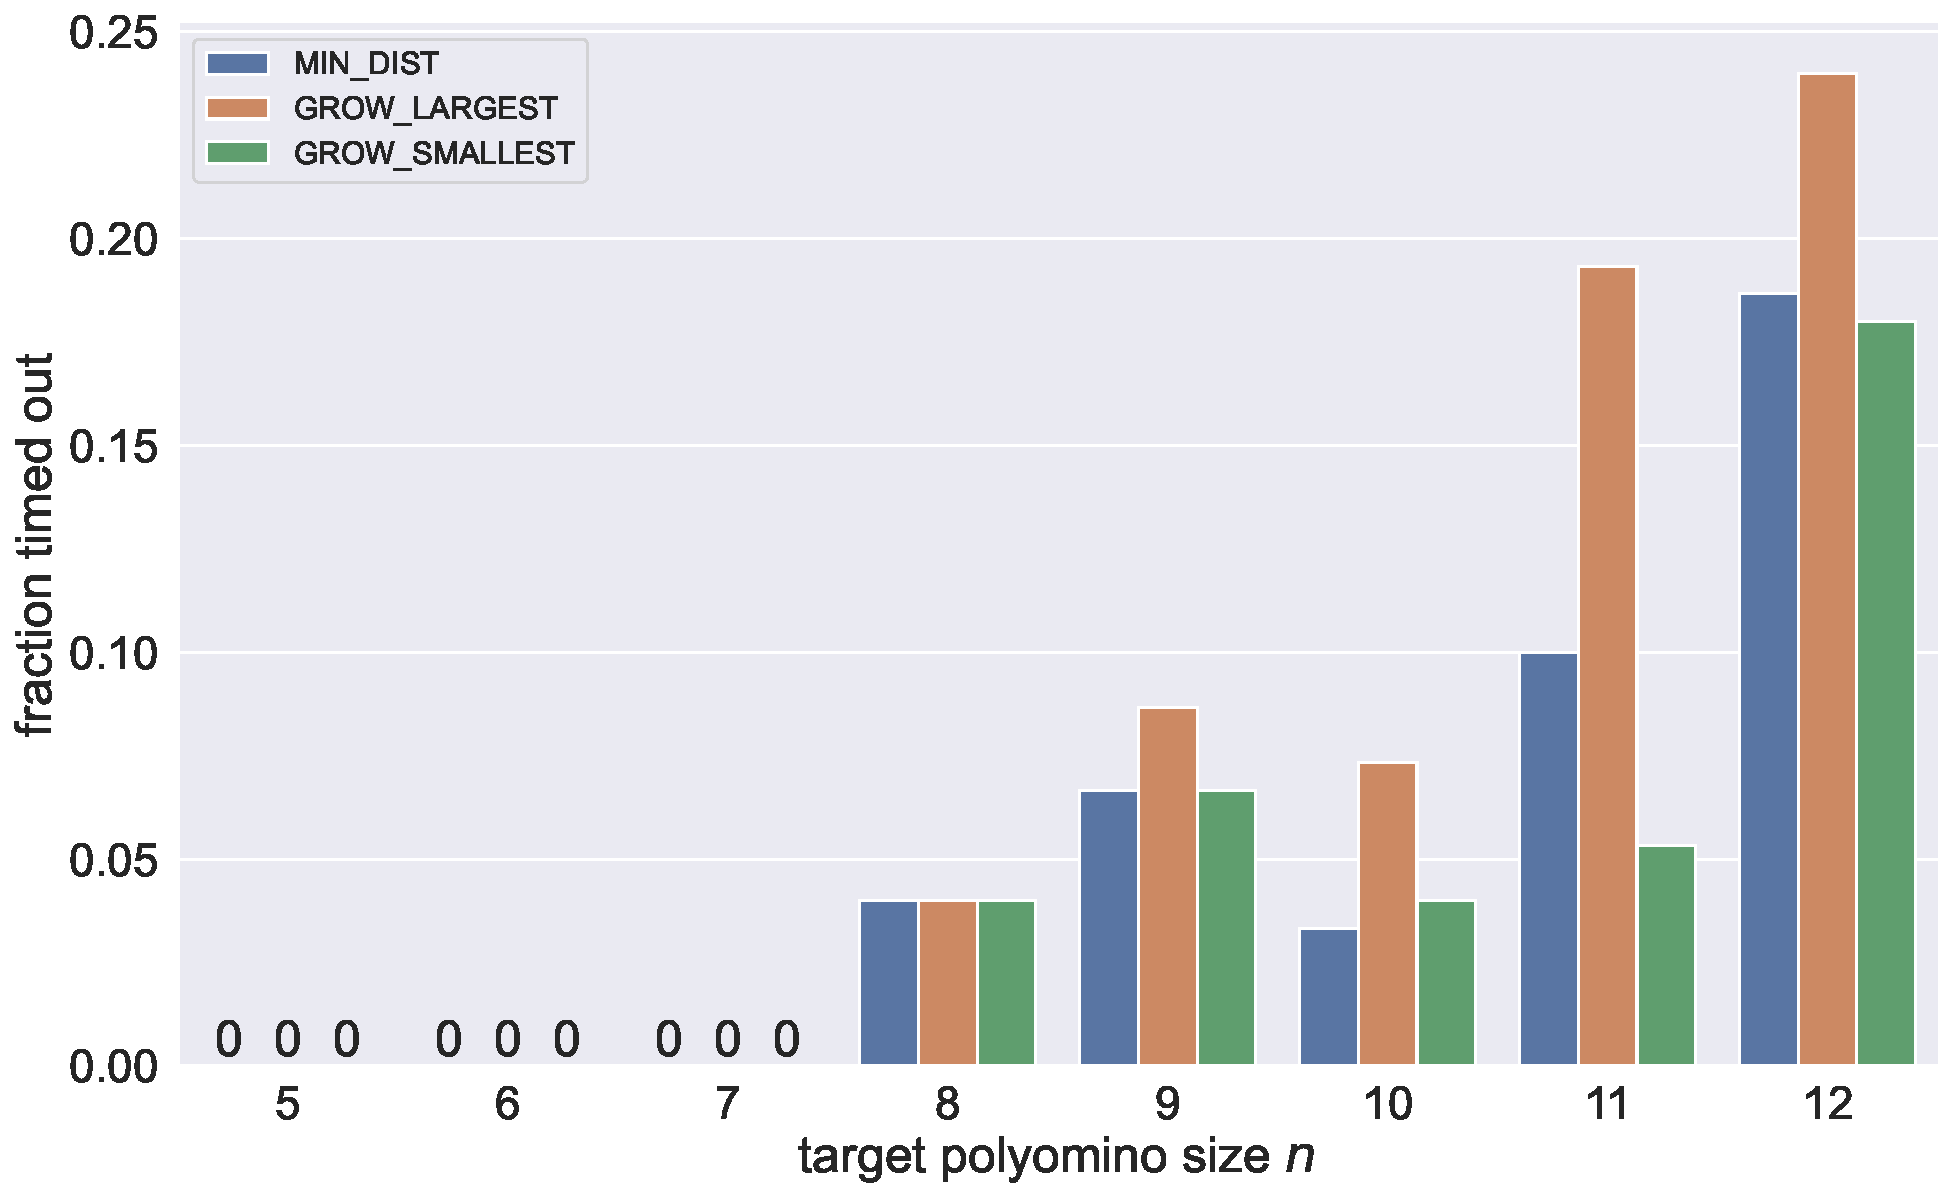
\includegraphics[width=0.9\textwidth]{figures/plots/AFN_timeout.pdf}
		\caption{Fraction of plans that timed out.}
		\label{fig:AFN_timeout}
	\end{subfigure}
	\caption[Planning time and fraction of timeouts for increasing target size]{Planning time and fraction of timeouts for increasing target size $n$. All option sorting strategies are compared.}
	\label{fig:AFN_timestats}
\end{figure}

\autoref{fig:AFN_time} shows the distribution of planning time and \autoref{fig:AFN_timeout} the fraction of timed out instances.
The construction of target polyominoes with sizes $5$ to $7$ can be planned in under $30$ seconds with just a few outliers exceeding this time.
Note the none of these instances timed out.

For target sizes above $7$ timeout failures first appear with roughly $5\%$ for $n = 8$ increasing to $20\%$ for $n=12$.
The planning time for $n = 12$ increases to $150$ seconds on average with a median of $100$ seconds.
With increasing $n$ a wider spread of planning time can be observed.
Outliers can reach planning times close to the timeout of $600$ seconds.

In terms of planning time the option sorting strategies make no noticeable difference.
For the fraction of timeouts growing the largest component often exceeds the other two strategies, clearly visible for $n=11$, where grow largest is at $20\%$ and the others under $10\%$ of plans timed out.


\paragraph{Plan Cost}

\begin{figure}
	\centering
	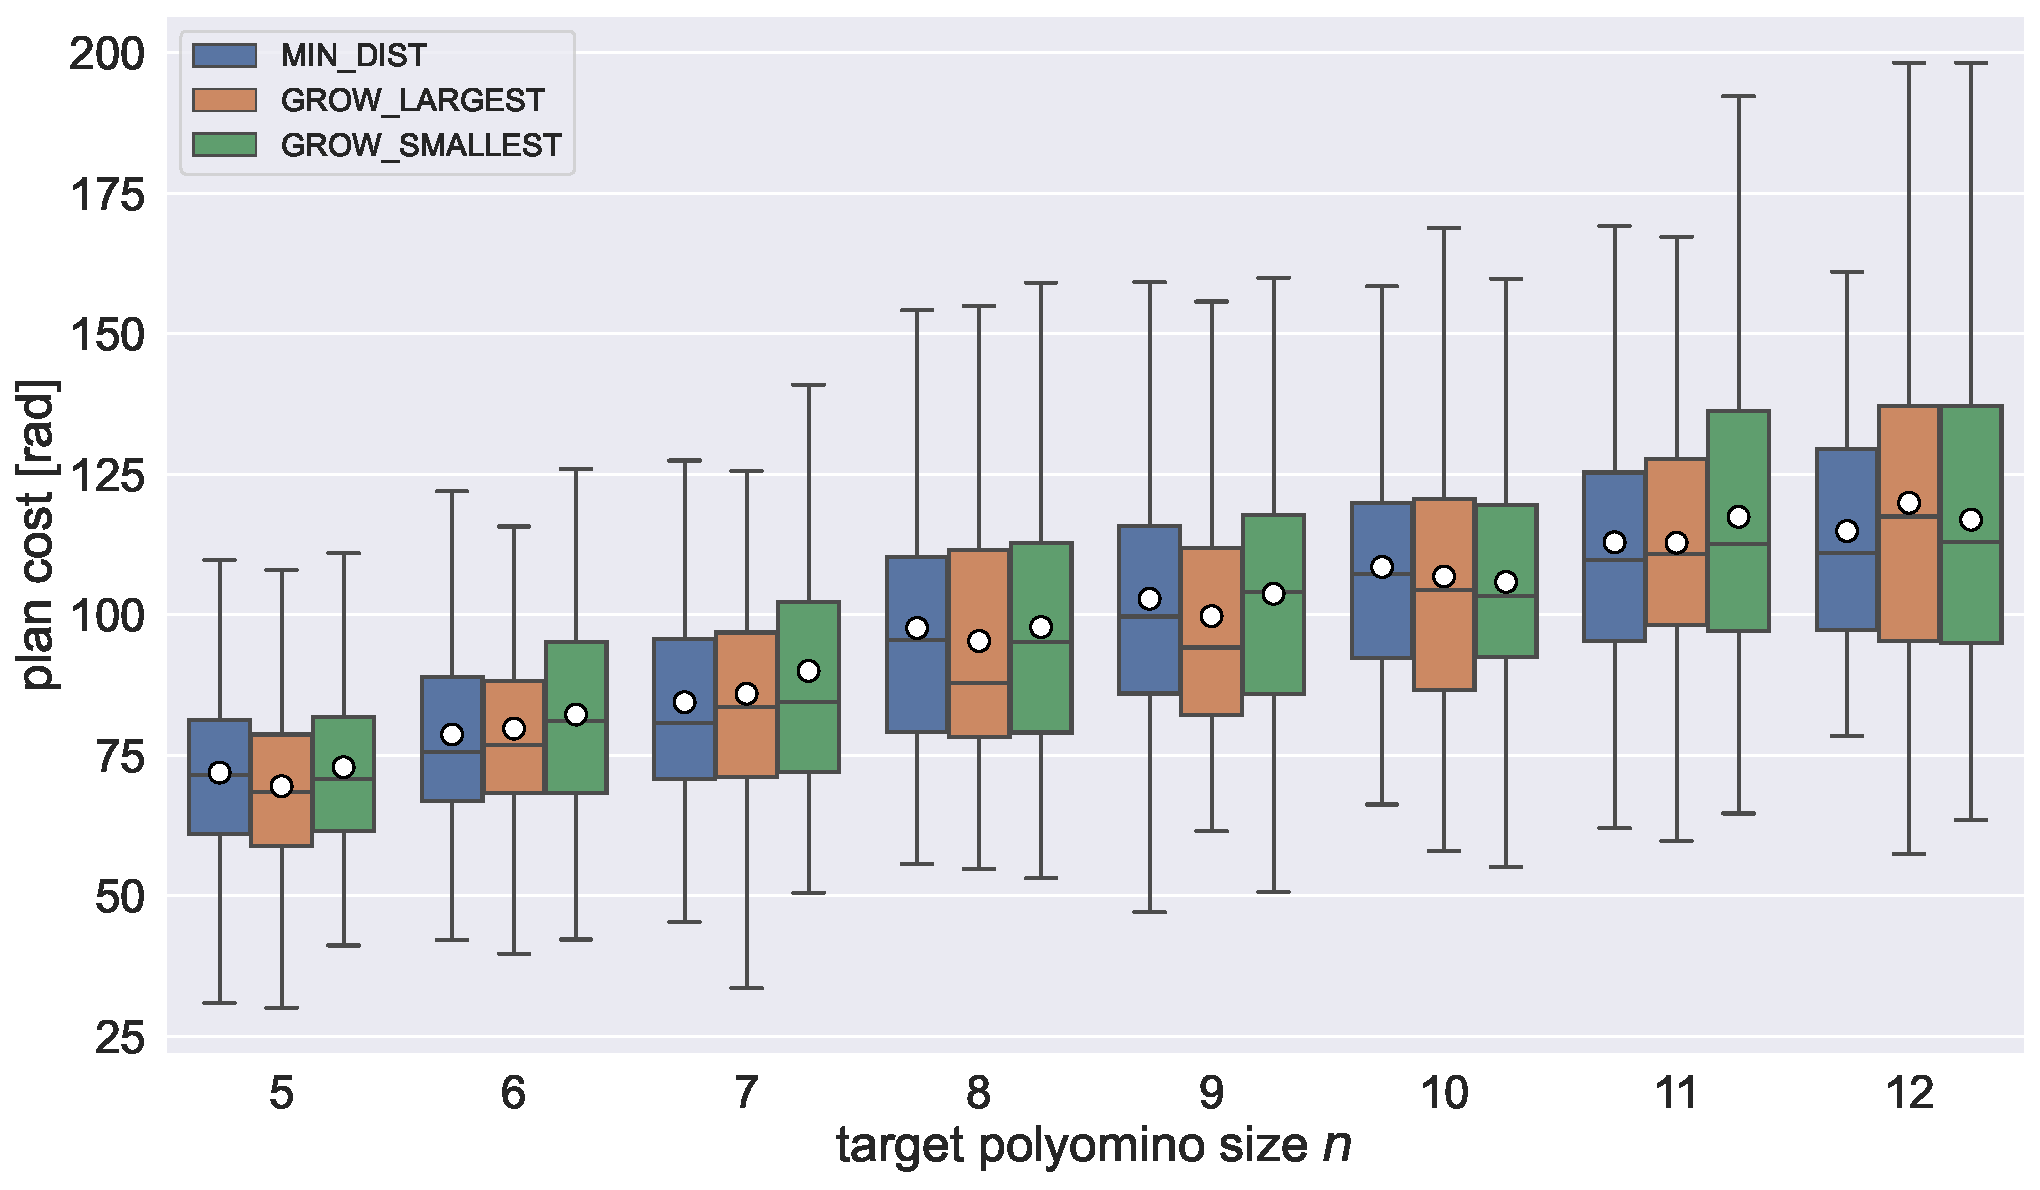
\includegraphics[width=0.9\textwidth]{figures/plots/AFN_cost.pdf}
	\caption[Plan cost for increasing size]{Plan cost in radians of successful plans for increasing target size $n$. All option sorting strategies are compared and outliers are omitted.}
	\label{fig:AFN_cost}
\end{figure}

\autoref{fig:AFN_cost} shows the rotational cost of plans that successfully assembled the target.
The cost increase slightly for bigger polyominoes, but the gradient seems to be flatting out for sizes $11$ and $12$.
Plan cost is generally in a range of $50$ to $150$ radians, which is the equivalent of $8$ to $24$ full longitude rotations of the magnetic field.
The different option sorting strategies do not impact the cost of a plan.

\paragraph{Planning Attributes}

\begin{figure}
	\centering
	\begin{subfigure}[b]{\textwidth}
		\centering
		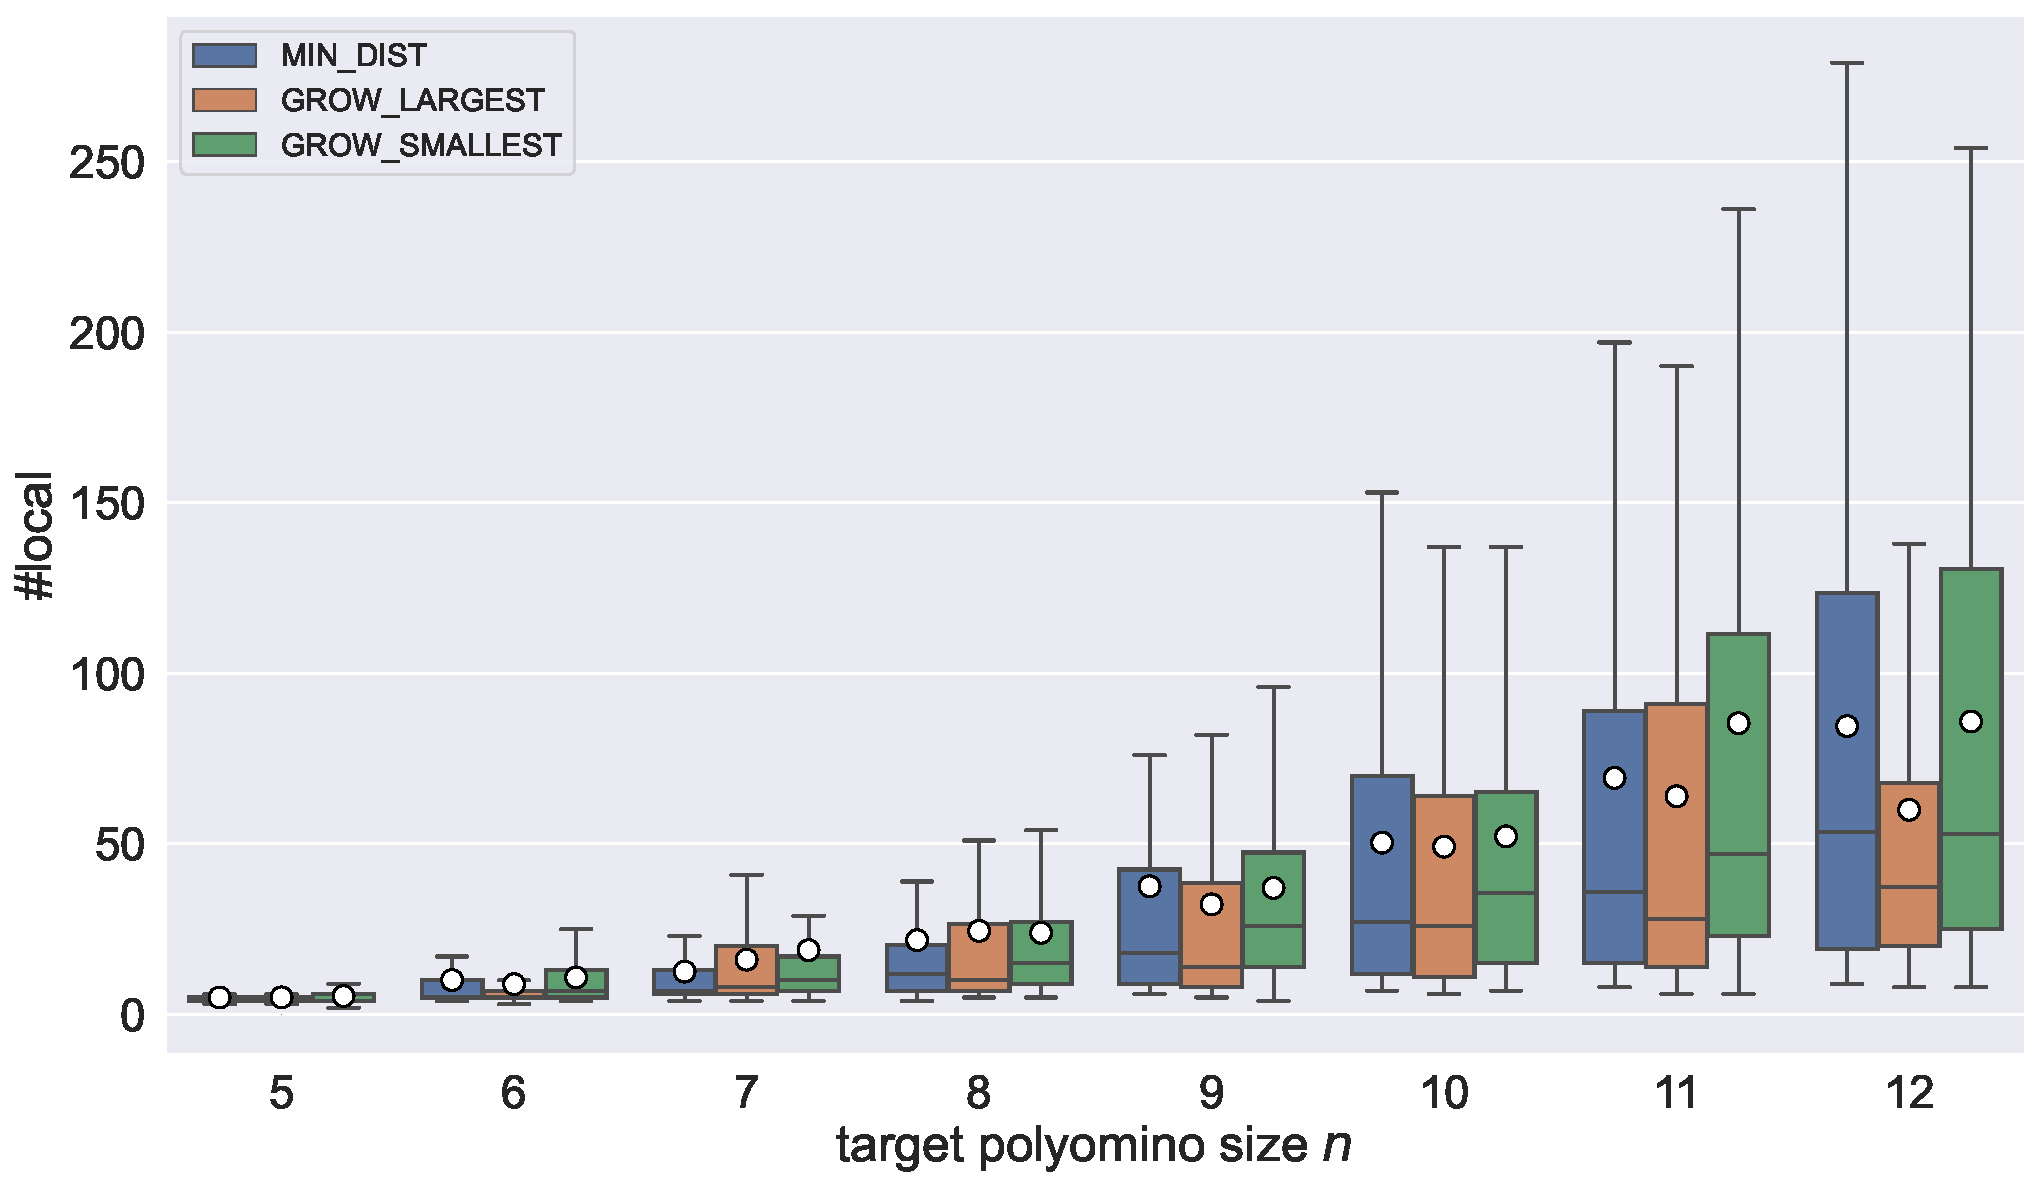
\includegraphics[width=0.9\textwidth]{figures/plots/AFN_nlocal.pdf}
		\caption{Number of simulated local plans.}
		\label{fig:AFN_nlocal}
	\end{subfigure}
	
	\begin{subfigure}[b]{\textwidth}
		\centering
		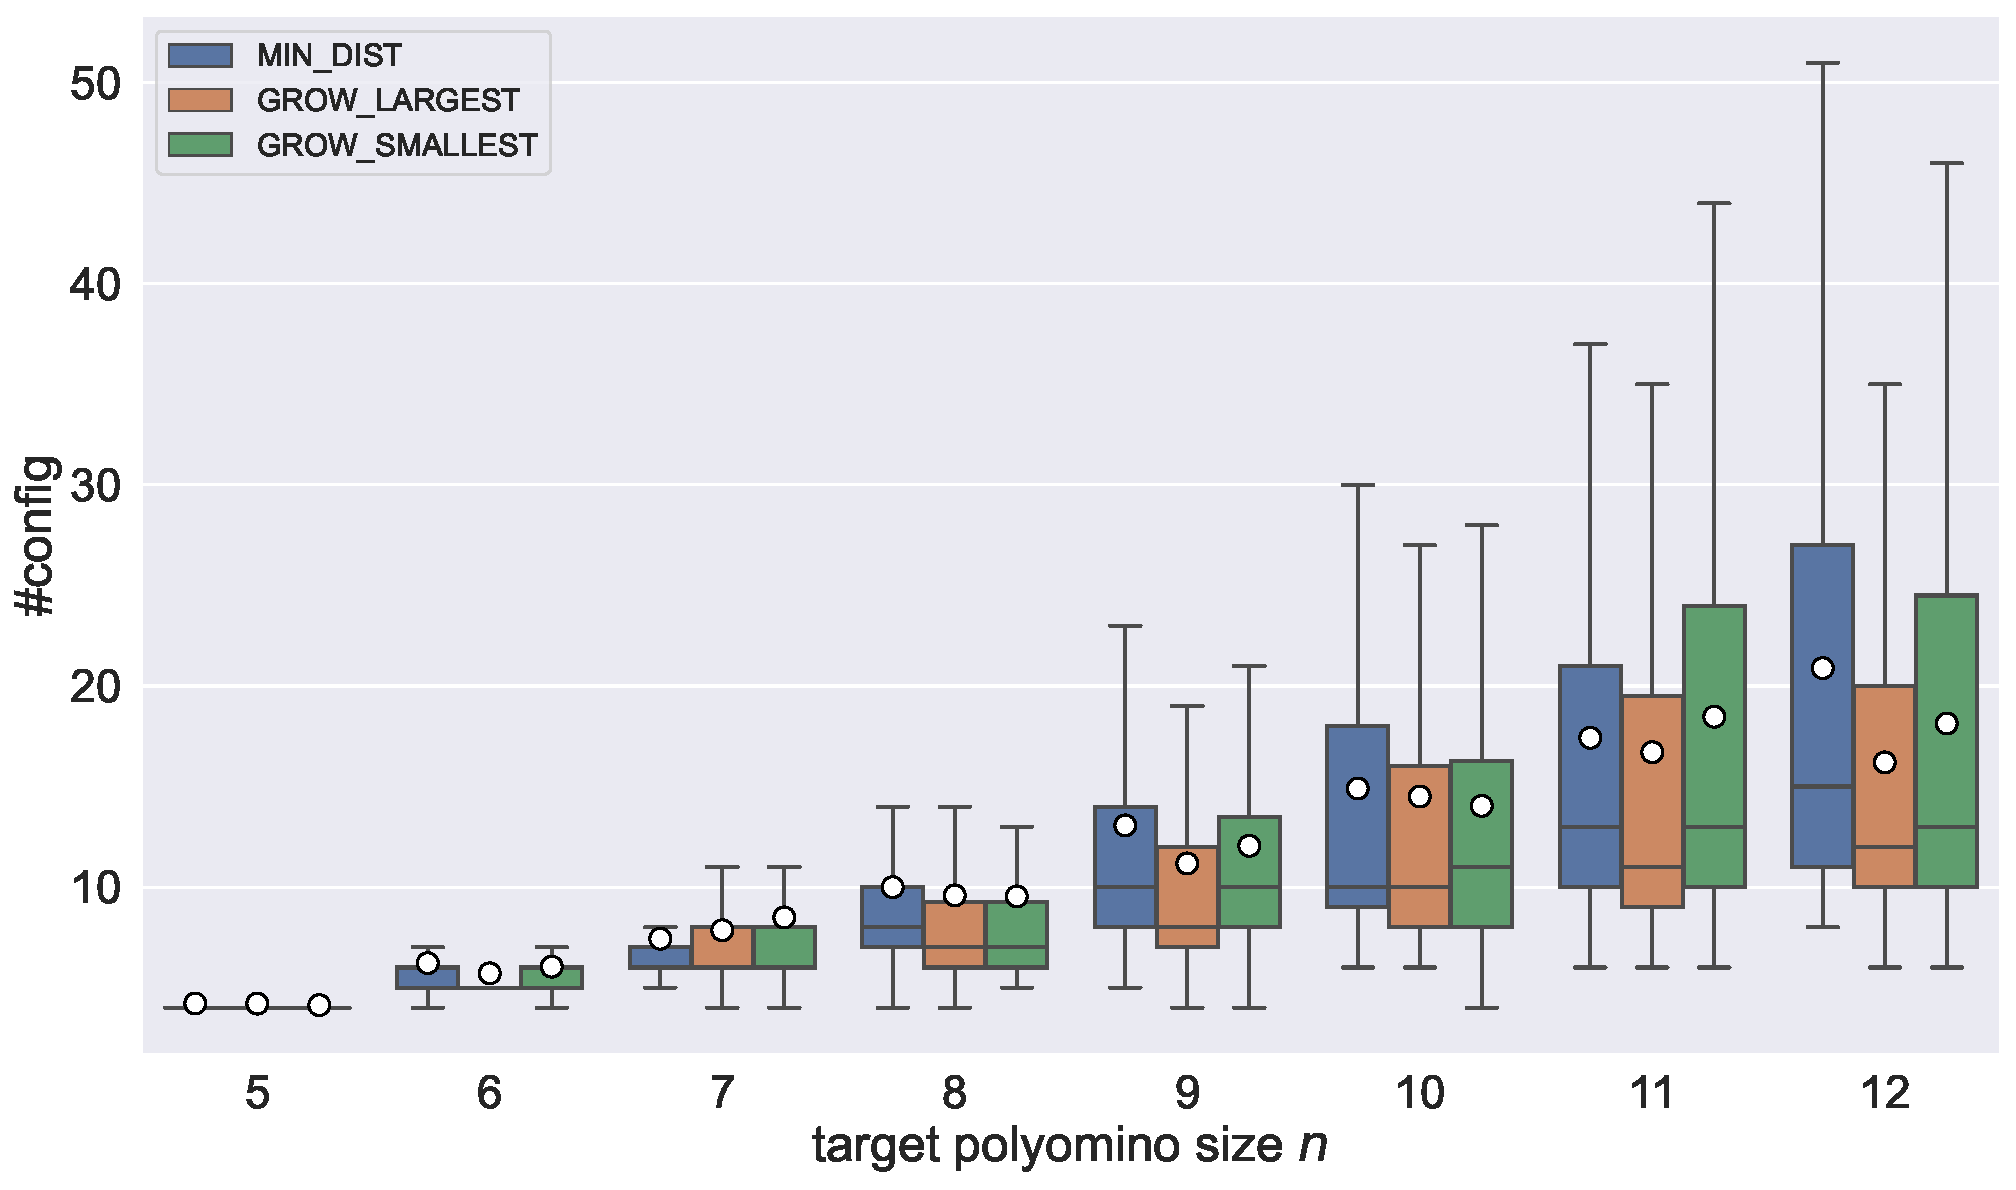
\includegraphics[width=0.9\textwidth]{figures/plots/AFN_nconfig.pdf}
		\caption{Number of explored configurations.}
		\label{fig:AFN_nconfig}
	\end{subfigure}
	\caption[Number of simulated local plans and explored configurations for increasing target size]{Number of simulated local plans $\#\textit{local}$ and explored configurations $\#\textit{config}$ for increasing target size $n$. Only plans that did not time out are shown and outliers are omitted for better readability. All option sorting strategies are compared.}
	\label{fig:AFN_planstats}
\end{figure}

\begin{figure}
	\centering
	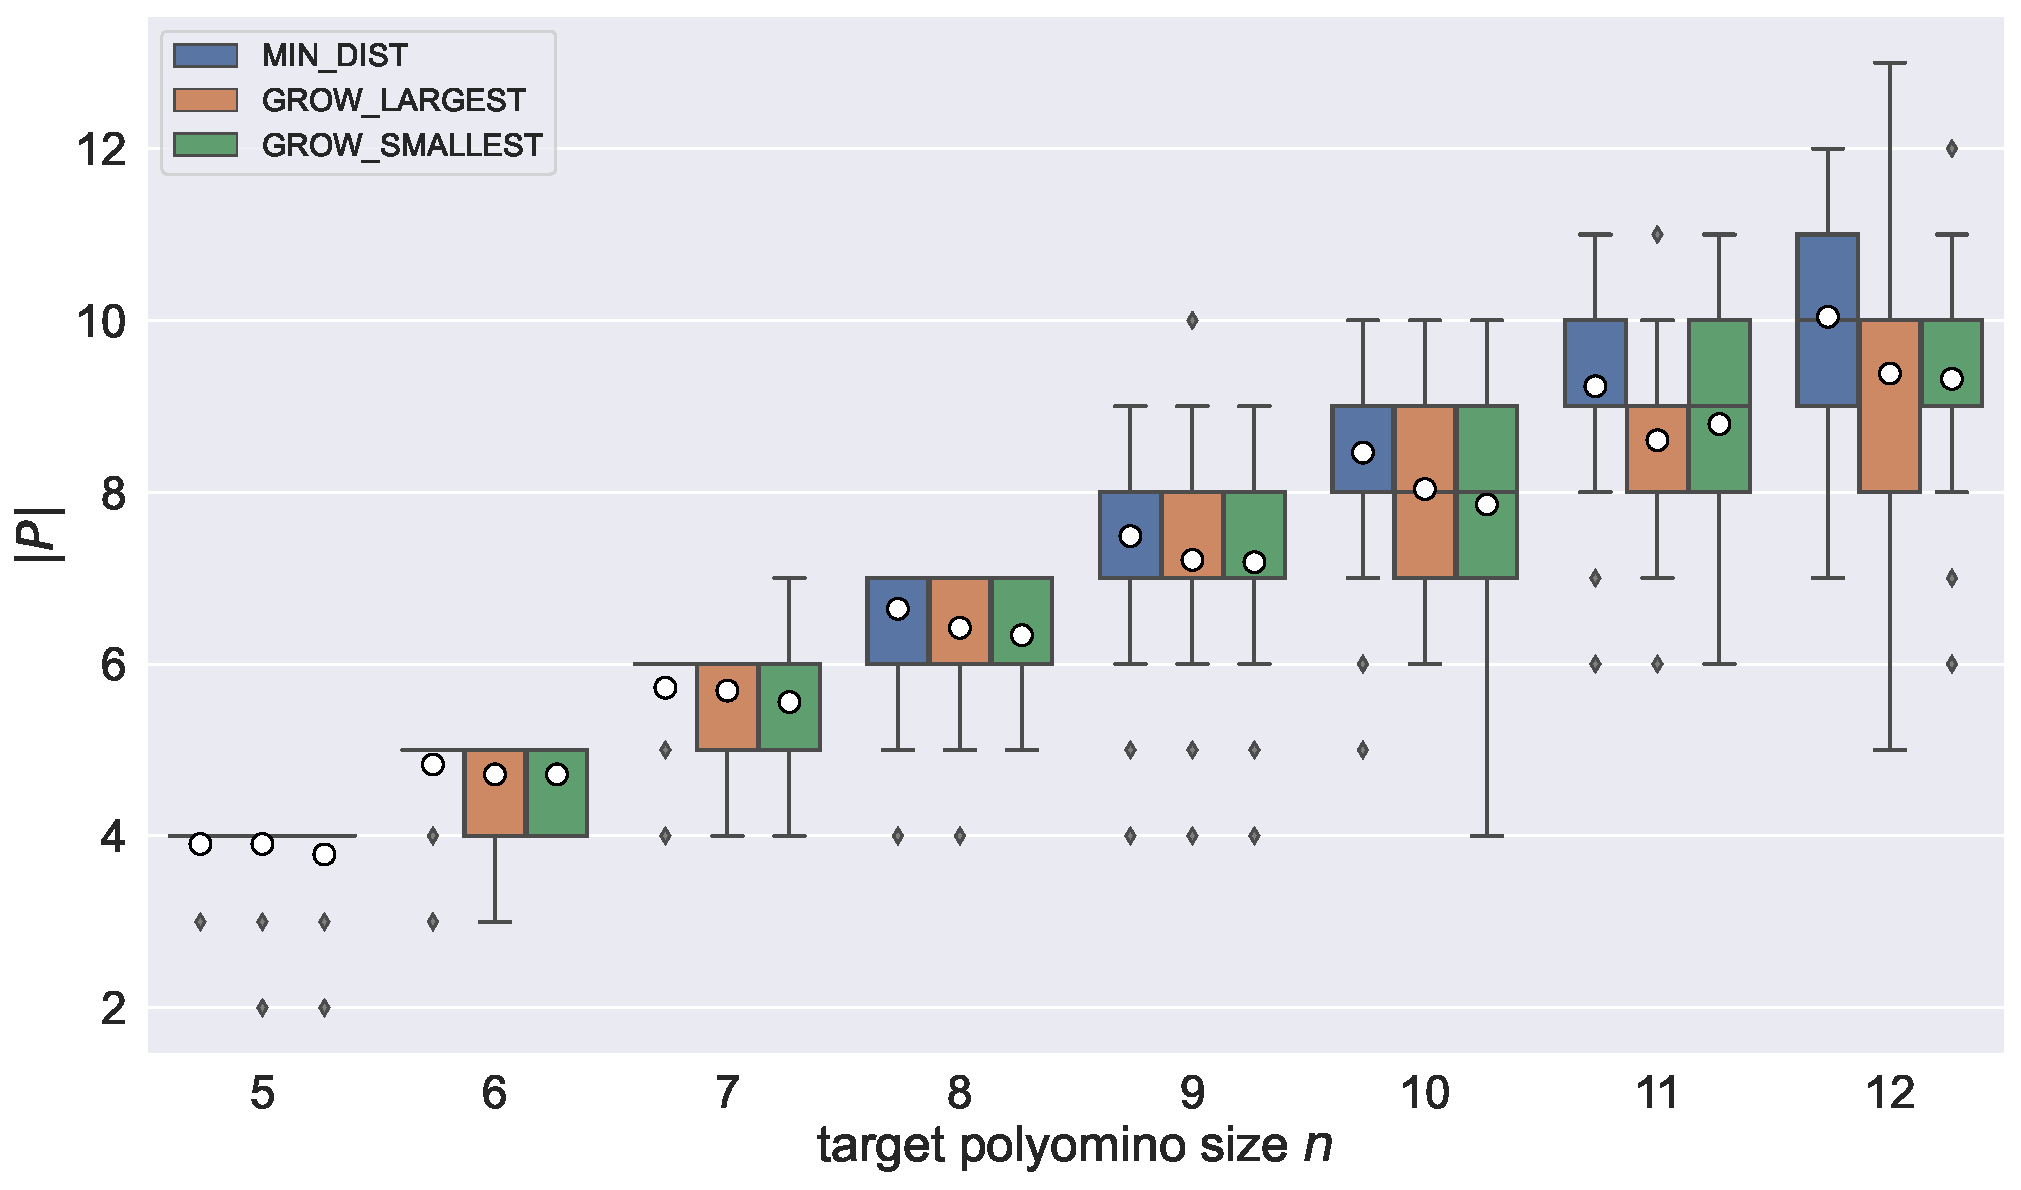
\includegraphics[width=0.9\textwidth]{figures/plots/AFN_ltg.pdf}
	\caption[Local plans in plan stack for increasing target size]{Local plans in plan stack $|P|$ for increasing target size $n$. Only successful plans are shown and all option sorting strategies are compared.}
	\label{fig:AFN_ltg}
\end{figure}


We analyze the number of simulated local plan $\#\textit{local}$ and the number of explored configuration $\#\textit{config}$ in \autoref{fig:AFN_planstats}.
The number of local plans contained in the plan stack of the resulting global plan $|P|$ is evaluated in \autoref{fig:AFN_ltg}.

When a plan times out $\#\textit{local}$ and $\#\textit{config}$ only portray how many local plan and configurations can be explored within the timeout.
Numbers can reach values up to $\#\textit{local} = 1200$ and $\#\textit{config} = 300$.
Timed out instances are omitted in the plots of \autoref{fig:AFN_planstats}.

$\#\textit{local}$ increases for bigger target polyominoes.
On average the realistic best case of $n-1$ local plans (\autoref{sec:global_complex}) is exceeded.
For $n=8$ there are $25$, for $n=10$ about $50$ and for $n=12$ roughly $75$ local plans simulated on average.
For all $n$ the majority of instances are below the average.
Outliers can reach up to $250$ local plans.

$\#\textit{config}$ behaves similarly.
The averages exceed the realistic best case of $n$, for example $\#\textit{config} = 16$ with $n=12$.
In this example the global planner encountered at least $4$ dead ends during planning.
The small numbers of $\#\textit{config}$ show that our depth first search approach is able to assemble polyominoes by only exploring a small portion of the whole configuration space.

For the majority of instances the number of local plans in the plan stack is at $|P| = n-1$.
Layer skipping can be observed frequently whenever $|P| < n-1$.
Surprisingly, instances with $|P| > n-1$ can also be observed.
This should not be possible due to a TCSA graph depth of $n$.
An explanation for this is that polyominoes break during simulation and create polyomino sets, which are at the same or a lower depth than the initial set that the local planner started with.
This phenomenon becomes more frequent for $n \geq 9$.

The only noticeable difference between the option sorting strategies is that growing the largest component tends to have slightly lower numbers of $\#\textit{config}$.

%TODO-----Prove reading-------

\section{Assembly of Custom Polyominoes}
\label{sec:AFTS}

\begin{figure}
	\centering
	\begin{subfigure}[b]{\textwidth}
		\centering
		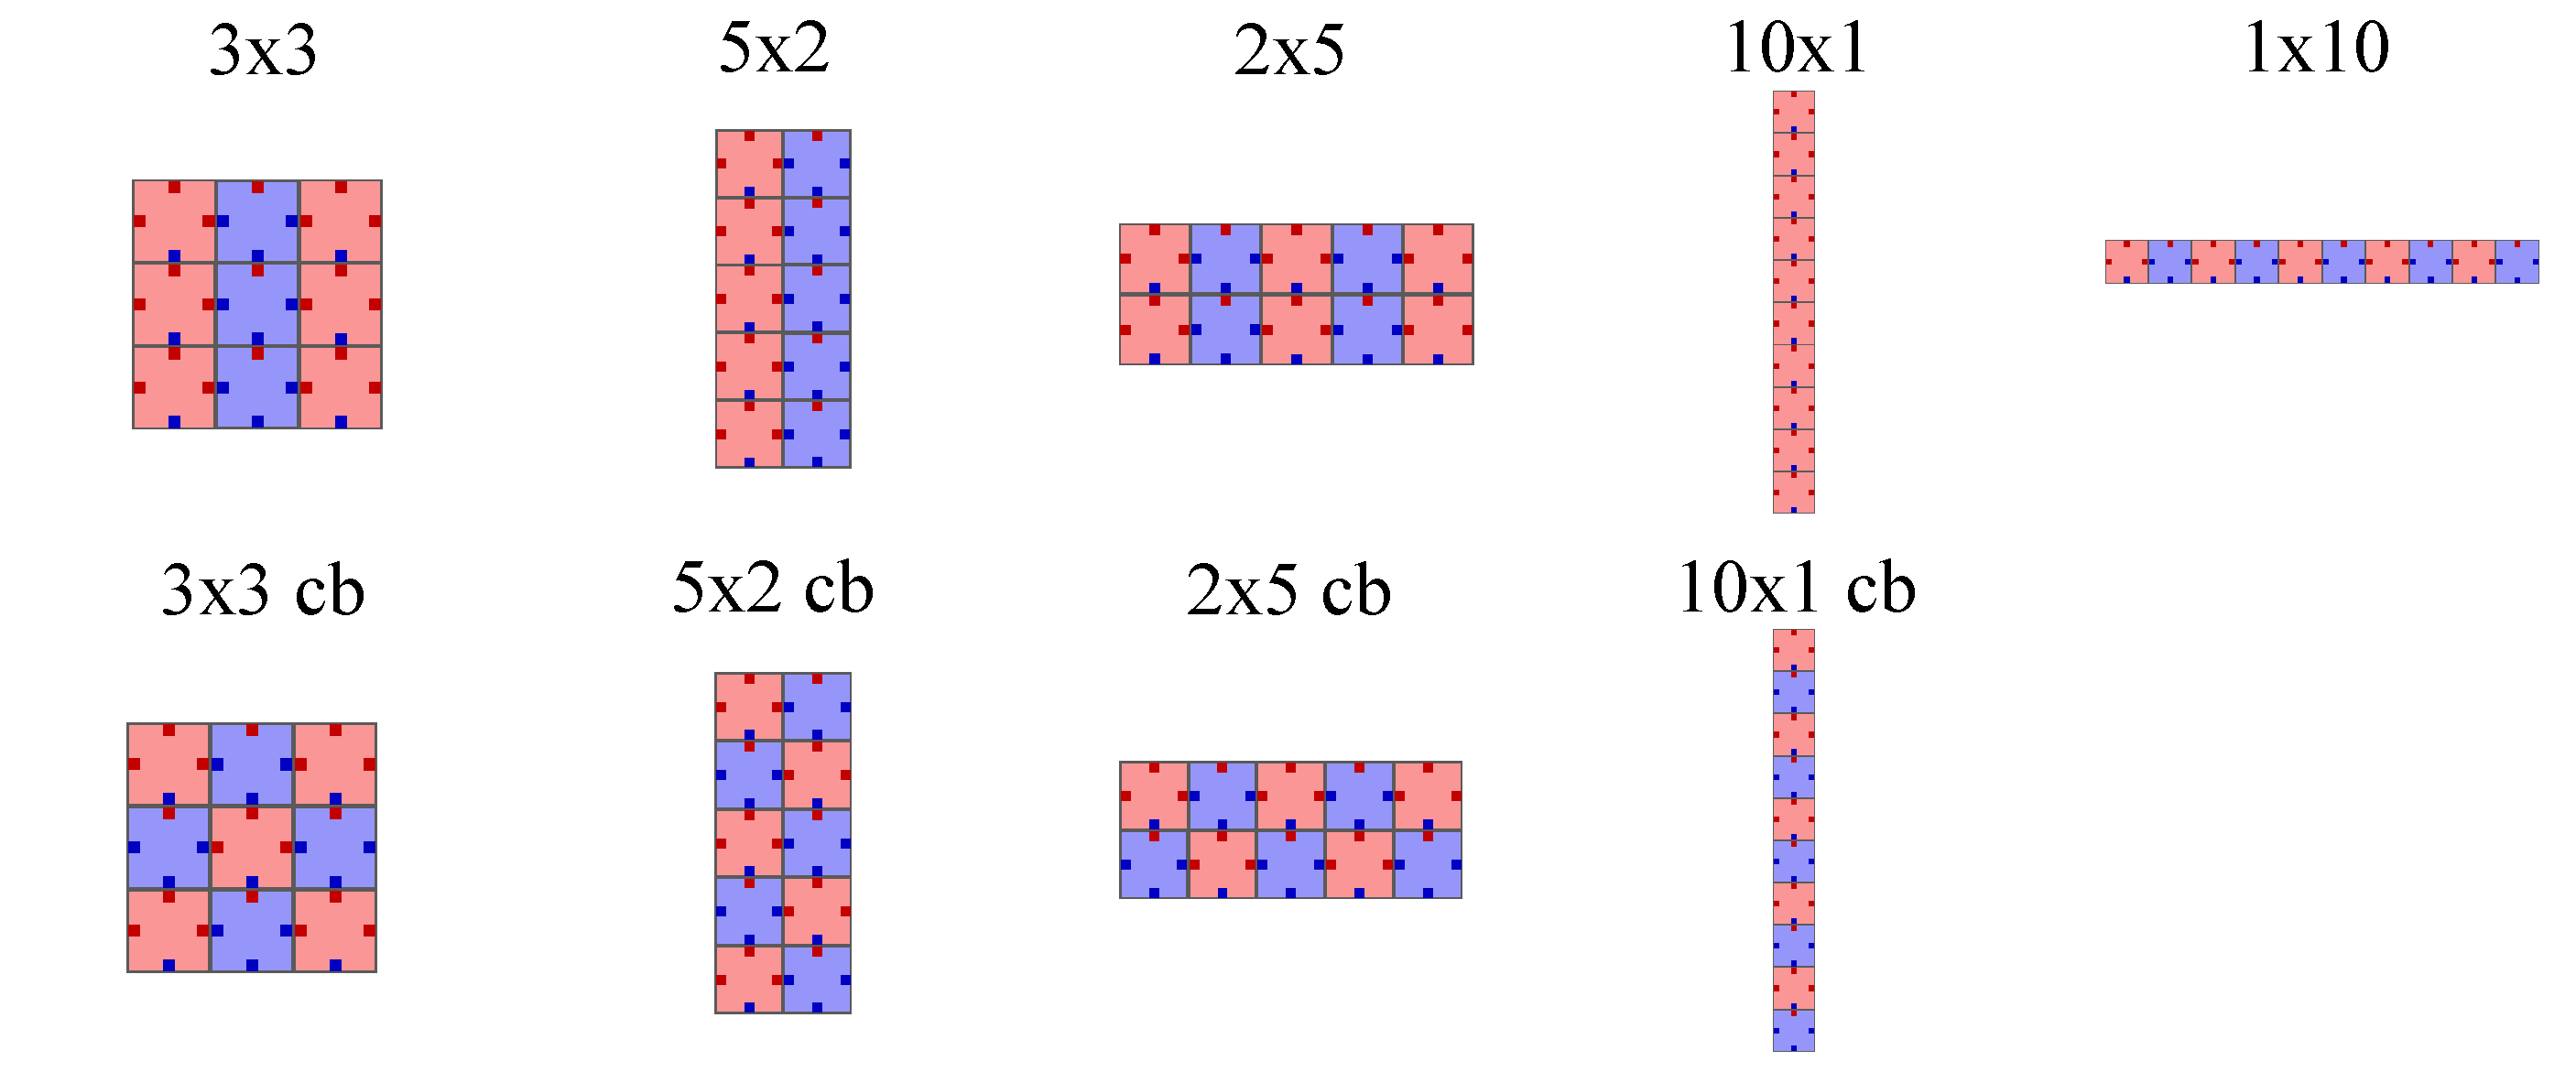
\includegraphics[width=0.8\textwidth]{figures/AFTS_cb_shapes.pdf}
		\caption{Rectangular polyominoes evaluated in \autoref{sec:w/h_pattern}. The checkerboard pattern is labeled with ``cb''. \hfill}
		\label{fig:AFTS_cb_shapes}
	\end{subfigure}
	\begin{subfigure}[b]{\textwidth}
		\centering
		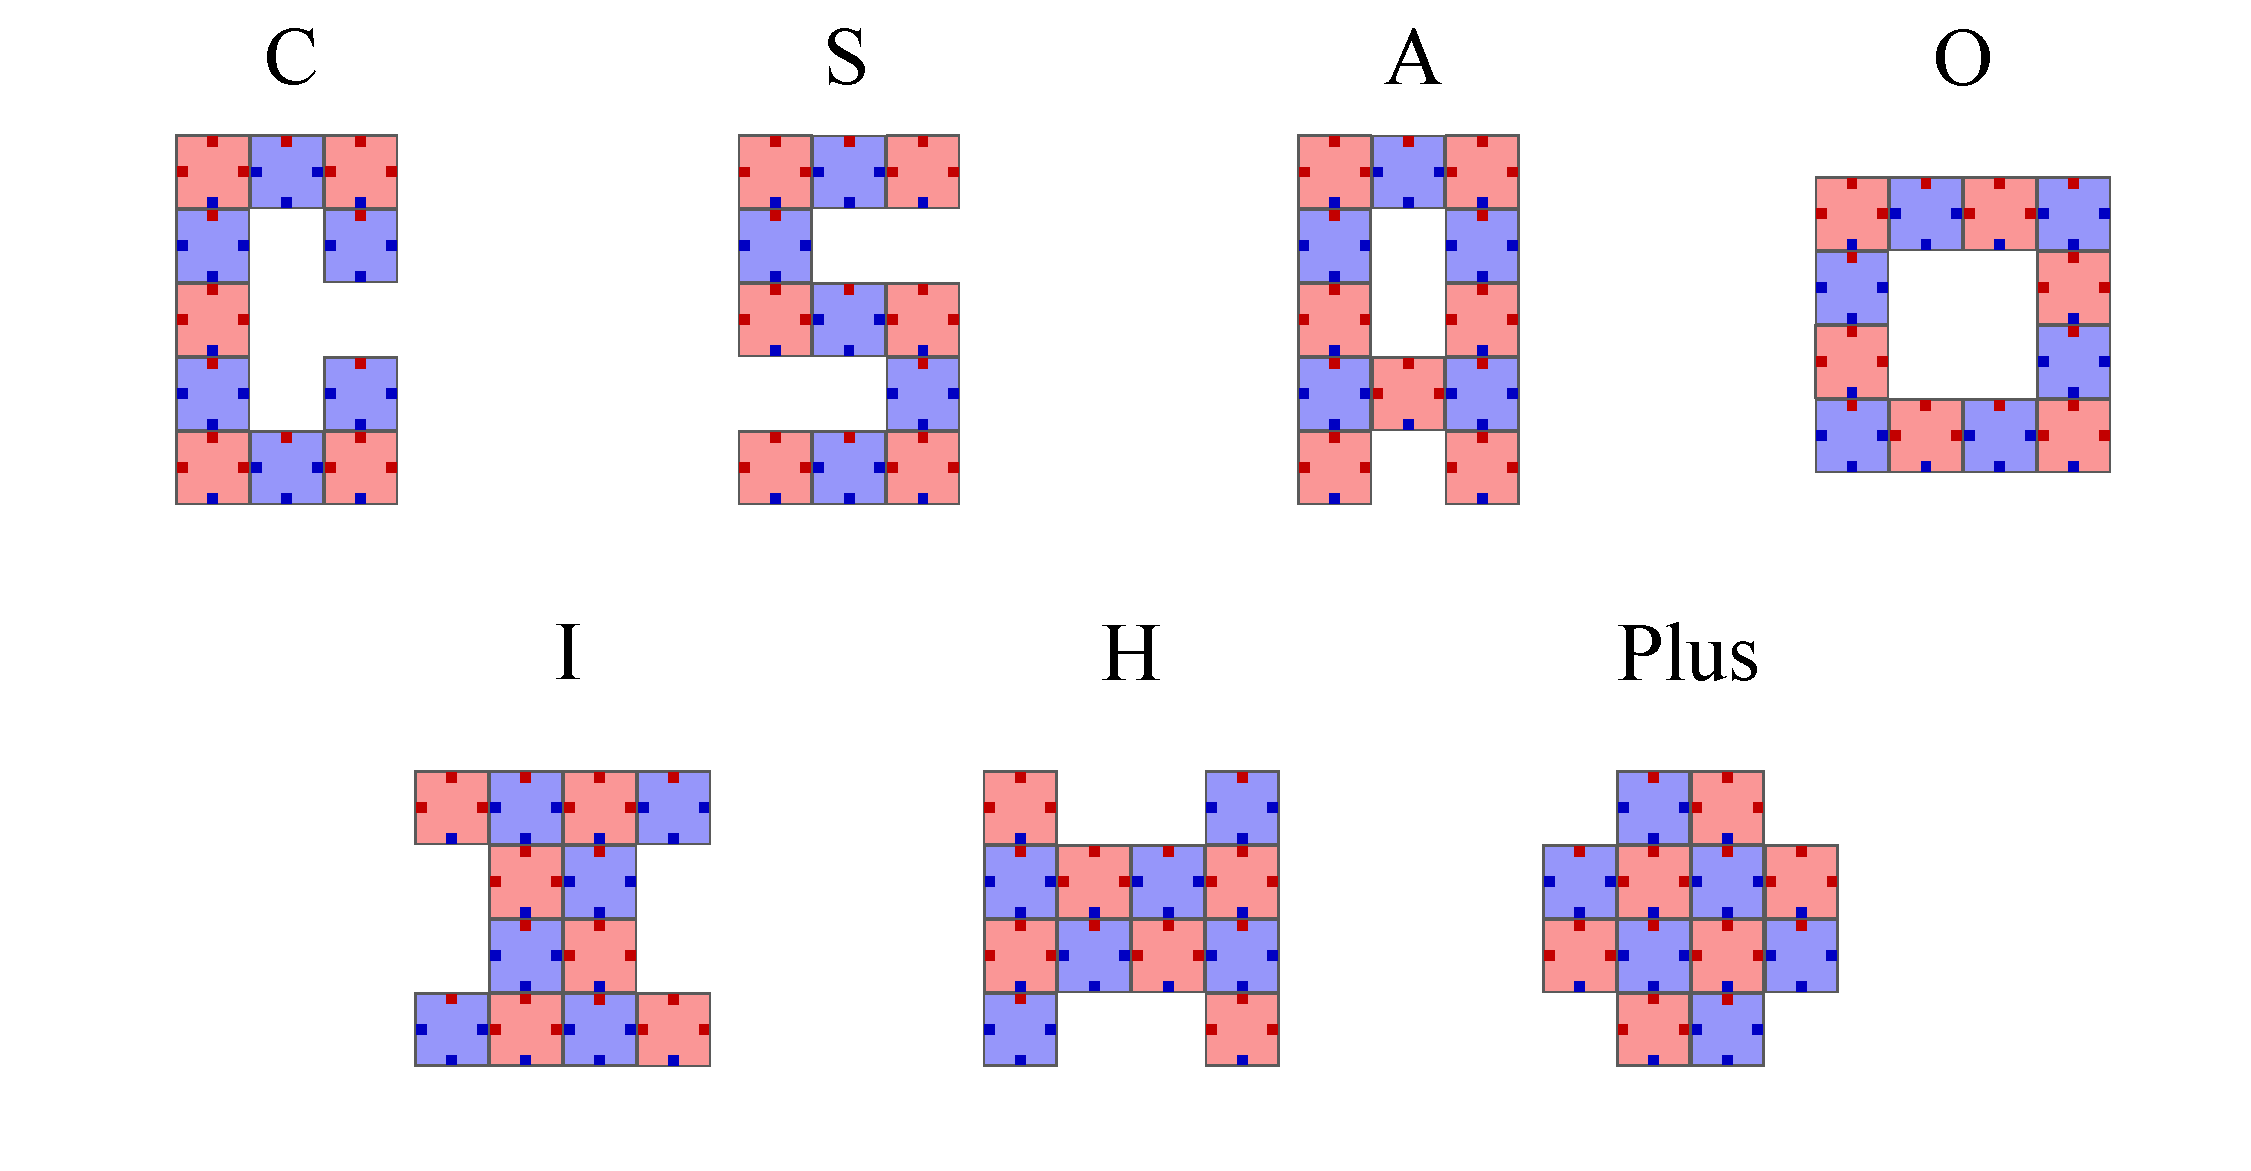
\includegraphics[width=0.7\textwidth]{figures/AFTS_sp_shapes.pdf}
		\caption{Special polyomino shapes evaluated in \autoref{sec:special_poly}.}
		\label{fig:AFTS_sp_shapes}
	\end{subfigure}
	\caption[List of manually designed polyominoes for experimenting]{List of manually designed polyominoes for experimenting.}
	\label{fig:AFTS_shapes}
\end{figure}

%TODO show number of tcsa nodes for all shapes

In this experiment manually designed polyominoes are assembled from multiple randomly generated initial configurations.
$100$ samples were taken for each custom polyomino with a workspace size of $50 r_C \times 50 r_C$.

In \autoref{sec:w/h_pattern} we focus on how rectangular polyominoes with varying width/height ratios influence planning time.
Furthermore we experiment with two patterns of red and blue for each polyomino.
The \textit{switching-column pattern} switches between red and blue cubes column vise and the \textit{checkerboard pattern} creates a checkerboard of single red and blue cubes.
A list of these polyominoes can be found in \autoref{fig:AFTS_cb_shapes}.

In \autoref{sec:special_poly} assembly of special polyomino shapes is examined. 
The polyominoes are listed in \autoref{fig:AFTS_sp_shapes}.
The polyominoes ``letter C'', ``letter S'' and ``letter A'' provide different caves.
``letter A'' additionally contains a hole. 

\subsection{Width/Height and Cube Pattern}
\label{sec:w/h_pattern}

\begin{figure}
	\centering
	\begin{subfigure}[b]{\textwidth}
		\centering
		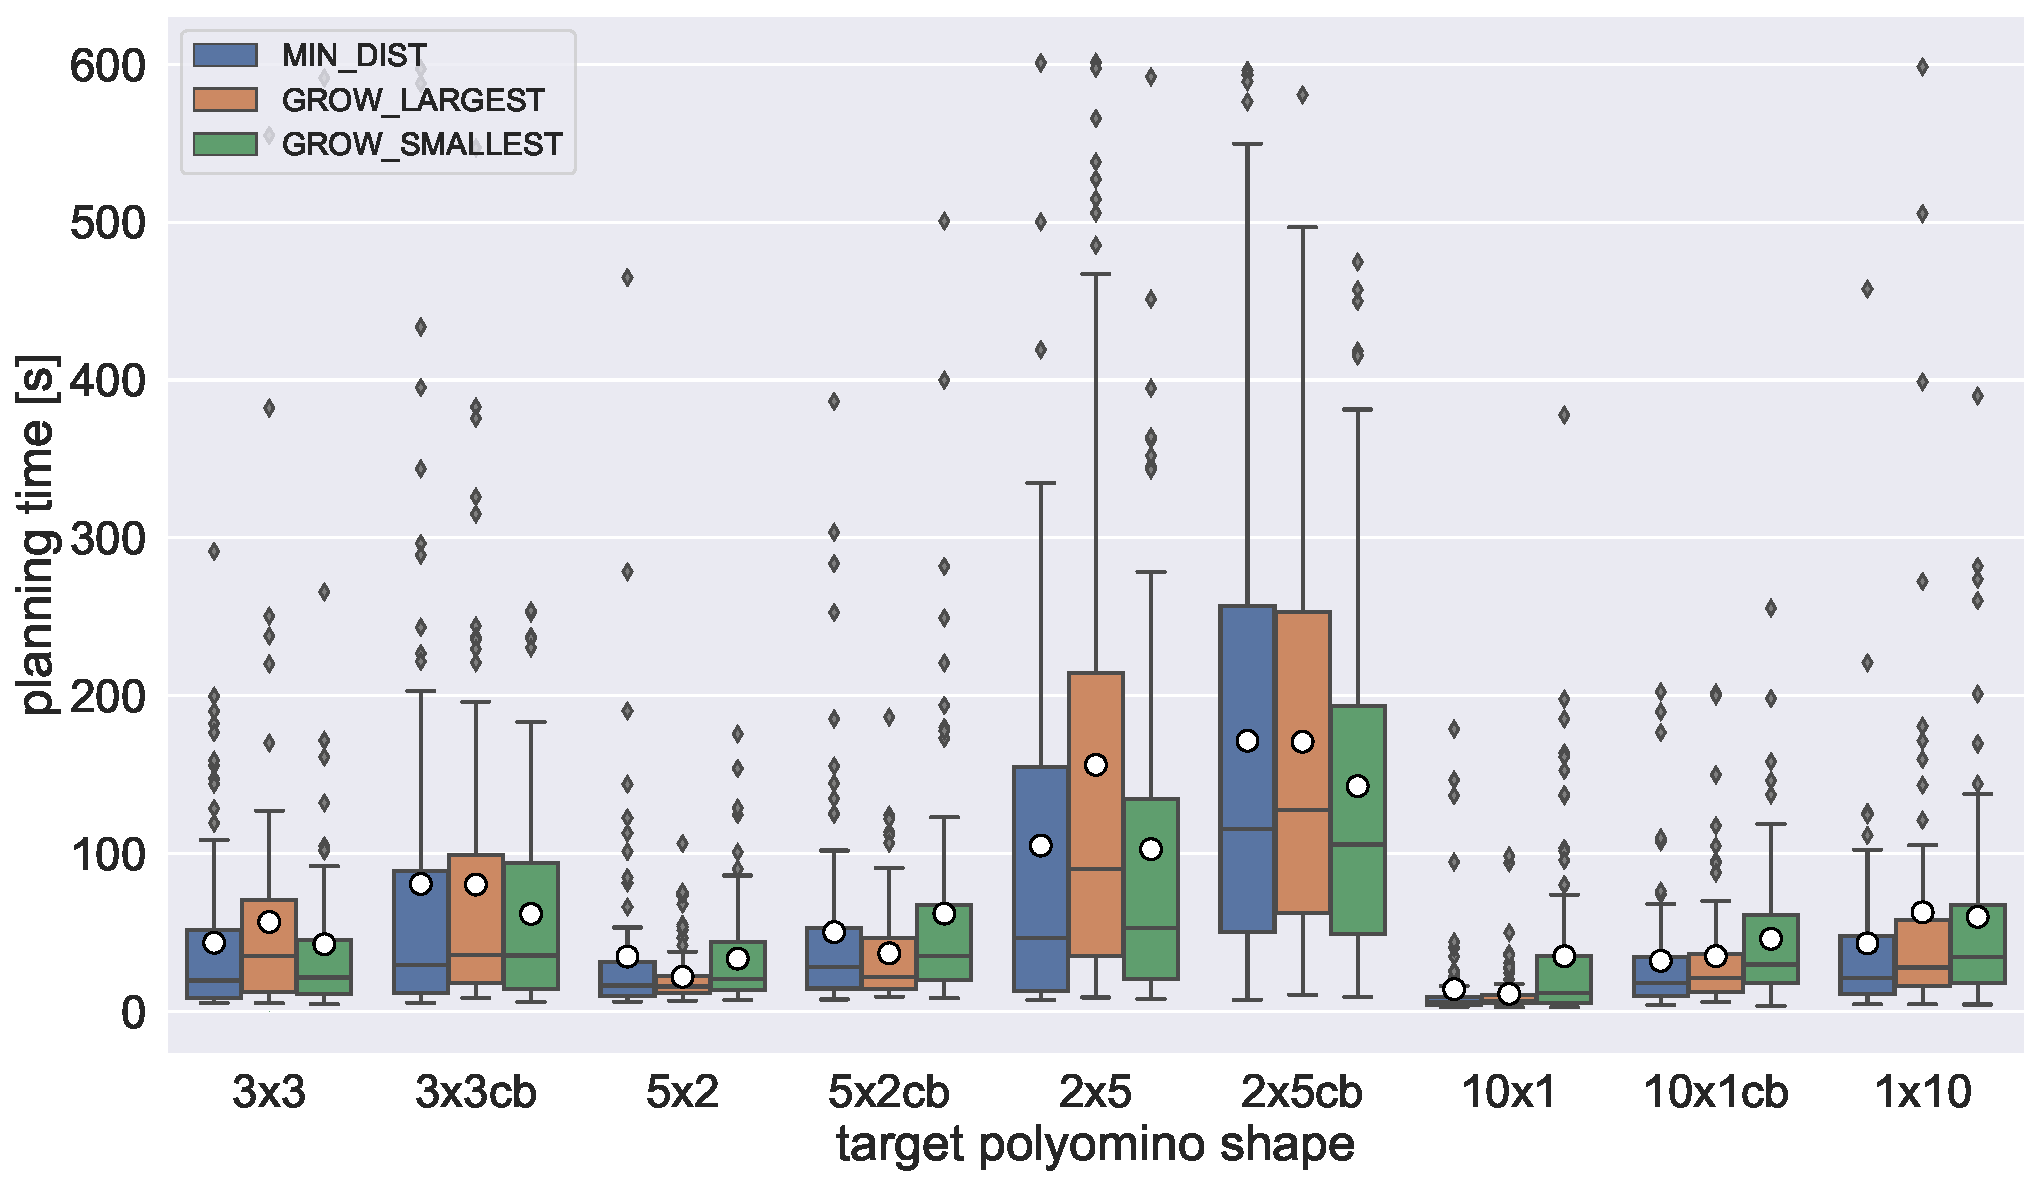
\includegraphics[width=0.9\textwidth]{figures/plots/AFTS_cb_time.pdf}
		\caption{Planning time in seconds. Only plans that did not time out are shown.}
		\label{fig:AFTS_cb_time}
	\end{subfigure}
	
	\begin{subfigure}[b]{\textwidth}
		\centering
		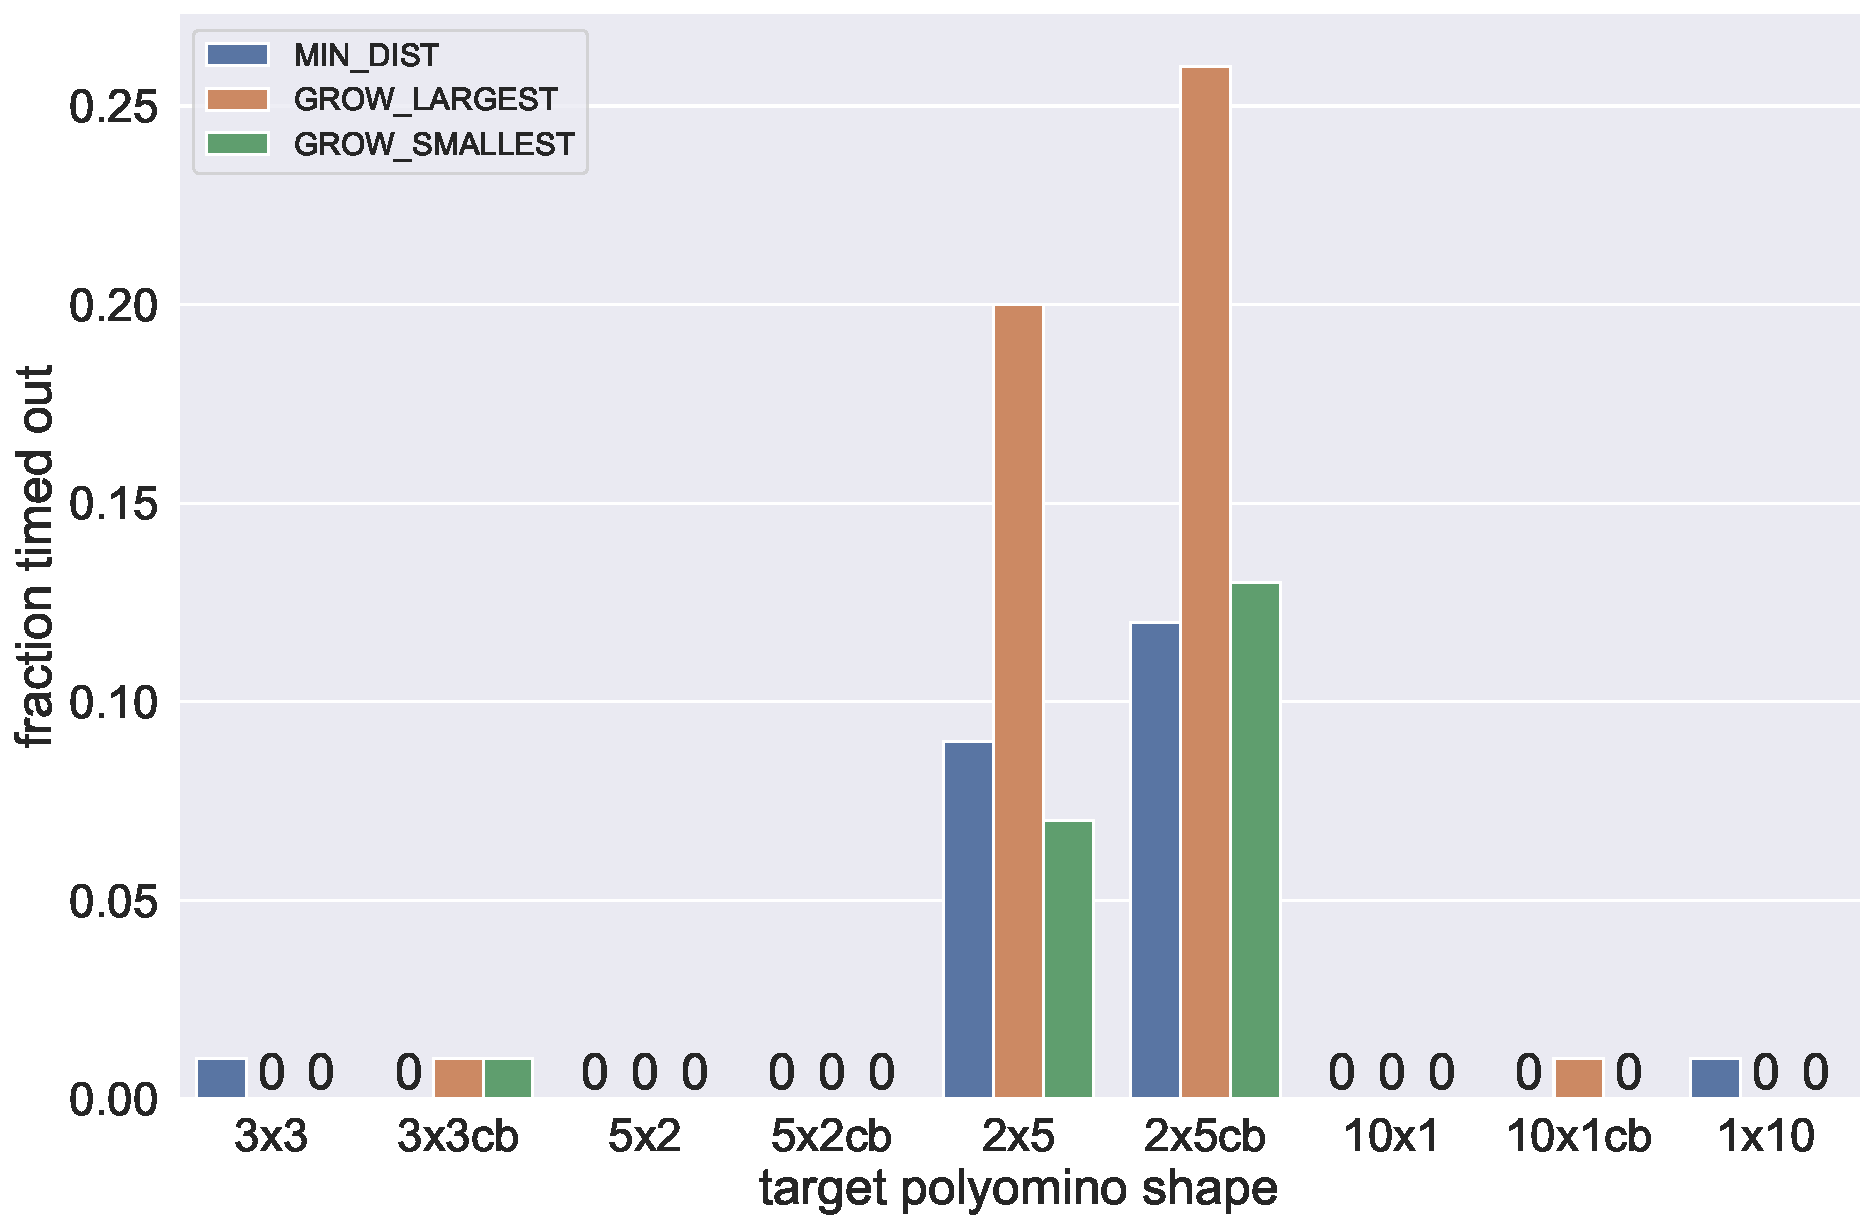
\includegraphics[width=0.9\textwidth]{figures/plots/AFTS_cb_timeout.pdf}
		\caption{Fraction of plans that timed out.}
		\label{fig:AFTS_cb_timeout}
	\end{subfigure}
	\caption[Planning time and fraction timed out for rectangular polyominoes]{Planning time and fraction timed out for rectangular polyominoes listed in \autoref{fig:AFTS_cb_shapes}. All option sorting strategies are compared.}
	\label{fig:AFTS_cb_timestats}
\end{figure}
%TODO shows shapes under plot

When comparing the two cube pattern in \autoref{fig:AFTS_cb_time}, the checkerboard pattern performs worst for all types of rectangular polyominoes.
It is not a huge difference, but still noticeable.
For instance, the ``3x3'' polyomino is on average at $50$ seconds planning time, while the ``3x3 cb'' polyomino is at 75 seconds with a wider spread and worst outliers.

Polyomino shapes with more height than width are faster to assemble.
``10x1'' is the best followed by ``5x2'', ``3x3'' and ``2x5''.
The same order persists for the checkerboard pattern.
Surprisingly the ``1x10'' polyomino breaks out of this order.
Its planning time lays between the ``5x2'' and the ``3x3''.
The ``2x5'' performs significantly worst than all other polyominoes.
While the majority of instances for all other shapes can be solved in under $100$ seconds, the ``2x5'' exceeds this time with a spread reaching up to $600$ seconds.

For the fraction of timed out plans shown in \autoref{fig:AFTS_cb_timeout}, the ``2x5'' is the only shape where $10\%$ to $20\%$ timeouts, depending on the option sorting strategy, can be observed.
All other shapes experience nearly no timeouts.

\subsection{Special Polyomino Shapes}
\label{sec:special_poly}


\begin{figure}
	\centering
	\begin{subfigure}[b]{\textwidth}
		\centering
		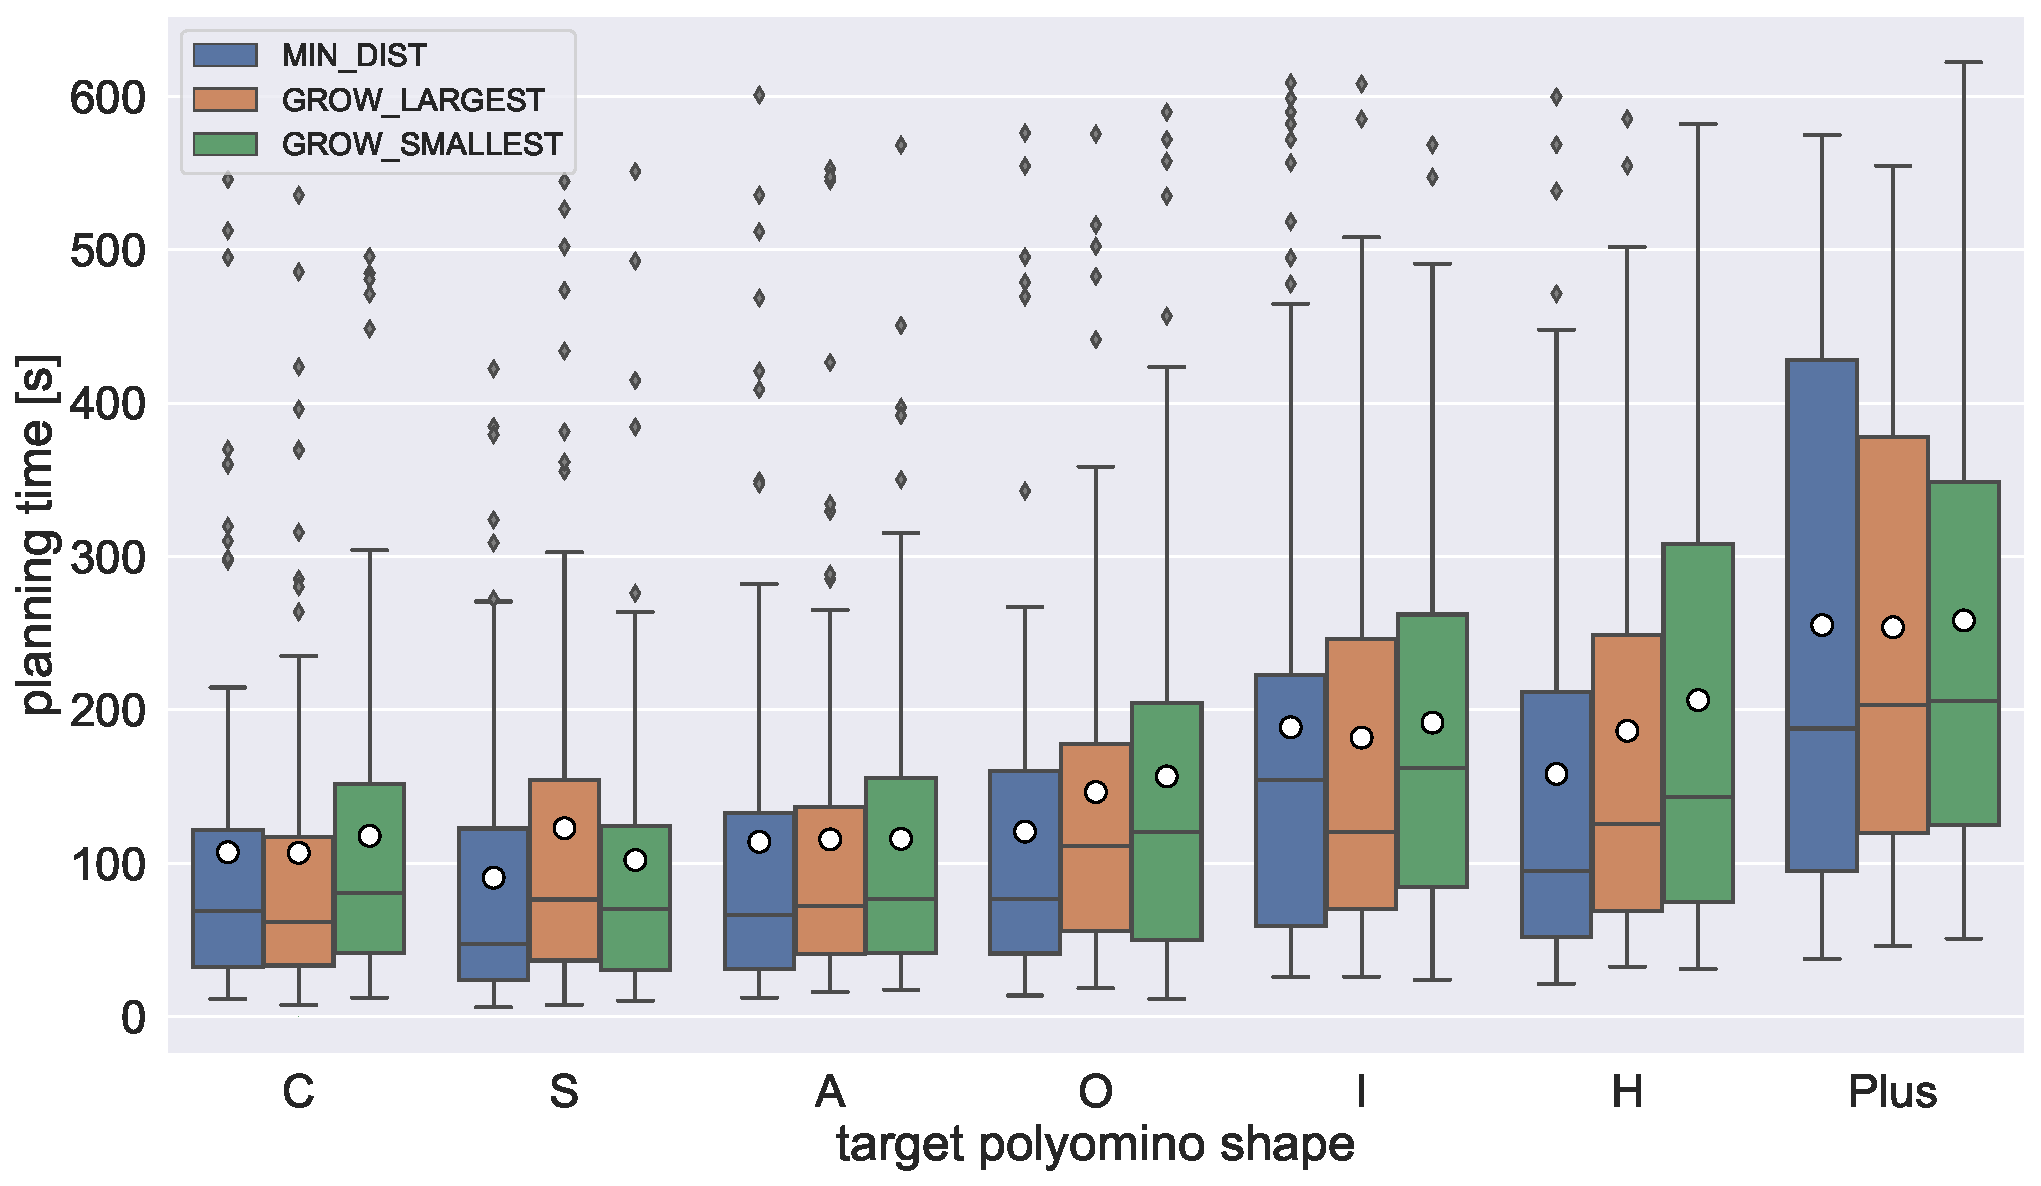
\includegraphics[width=0.9\textwidth]{figures/plots/AFTS_sp_time.pdf}
		\caption{}
		\label{fig:AFTS_sp_time}
	\end{subfigure}
	
	\begin{subfigure}[b]{\textwidth}
		\centering
		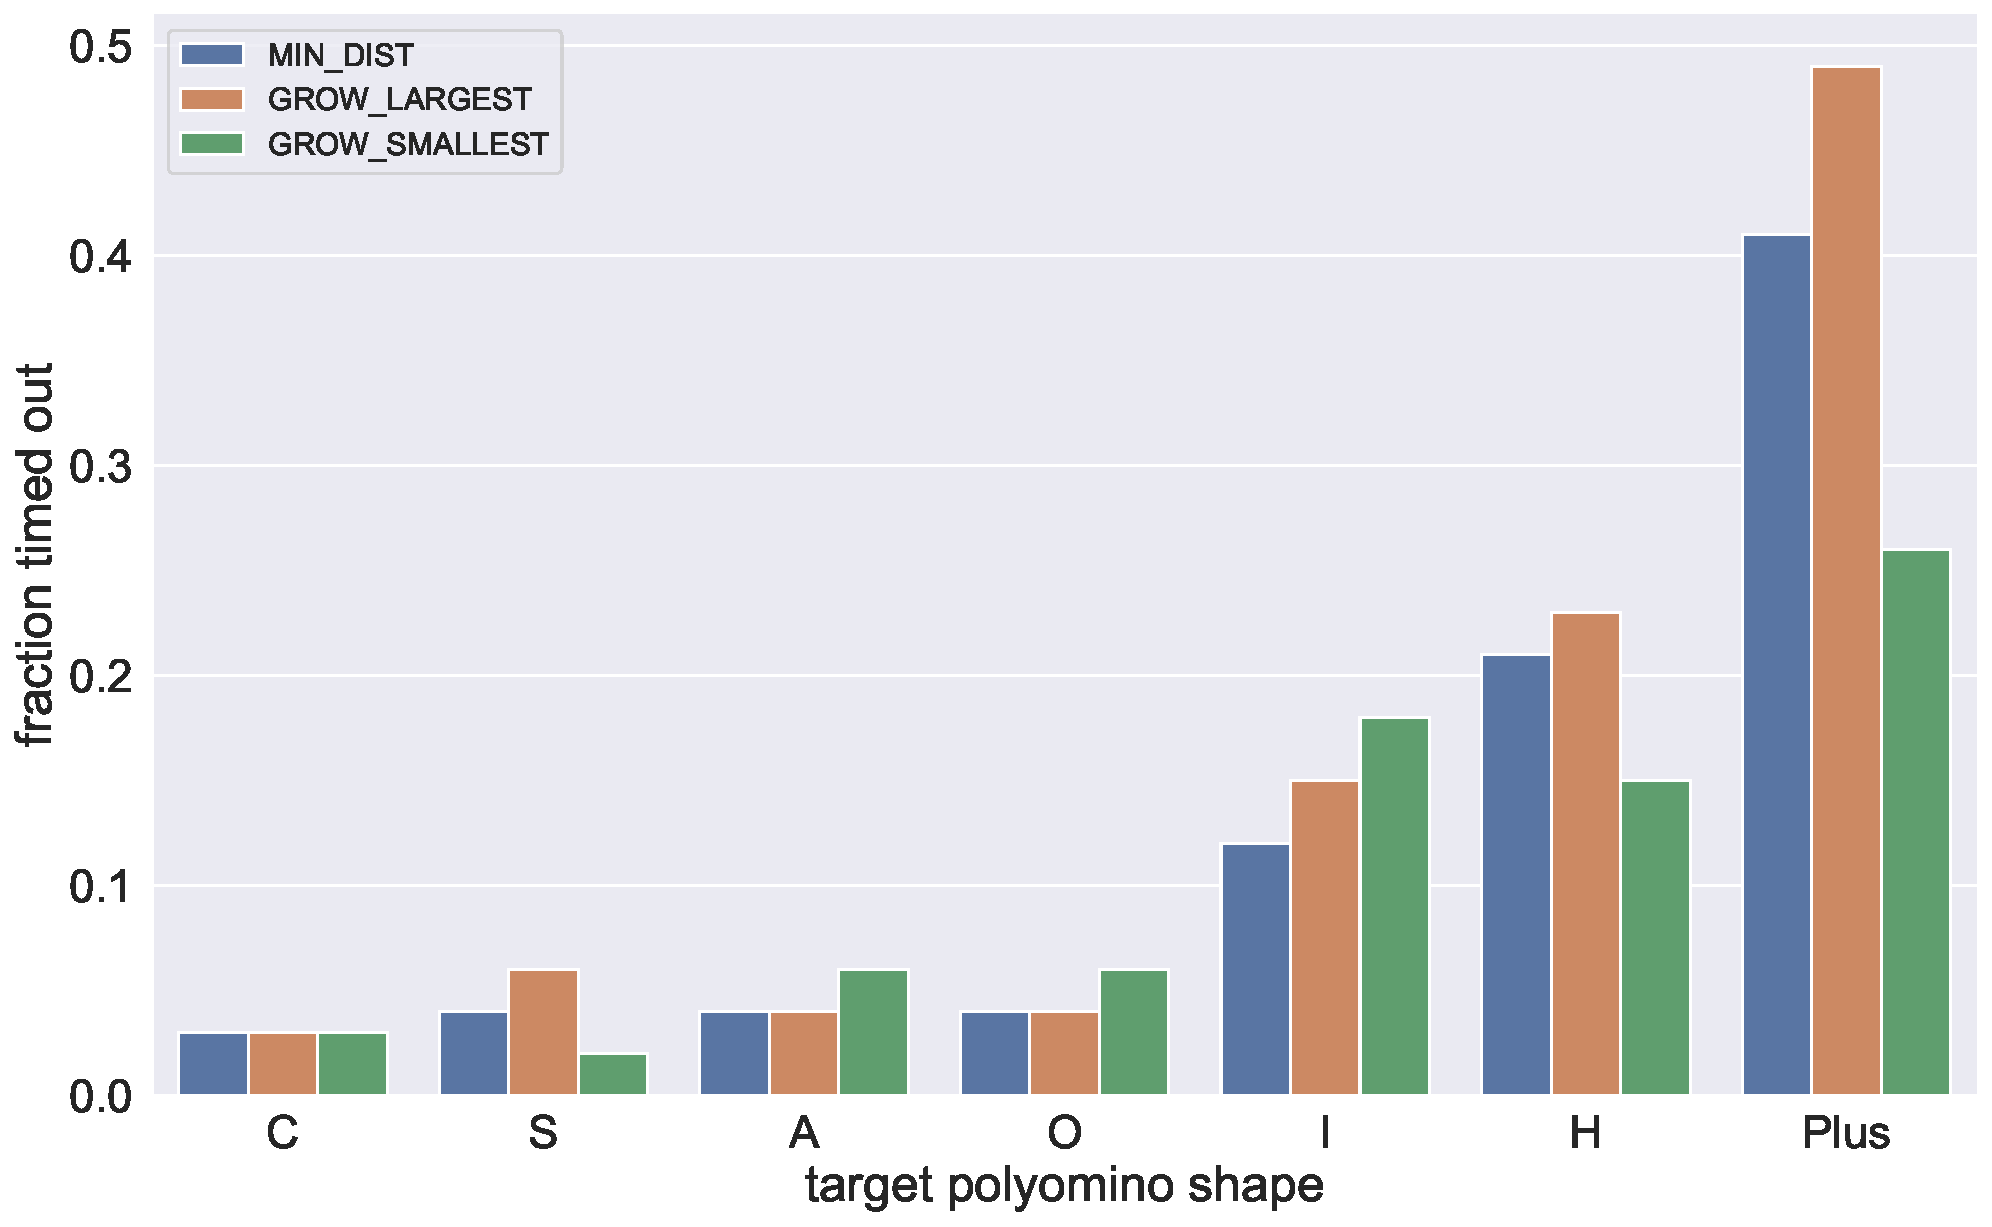
\includegraphics[width=0.9\textwidth]{figures/plots/AFTS_sp_timeout.pdf}
		\caption{}
		\label{fig:AFTS_sp_timeout}
	\end{subfigure}
	\caption[]{}
	\label{fig:AFTS_sp_timestats}
\end{figure}

Text




\section{Assembly in different Workspaces}
\label{sec:AFBS}

\begin{table}
	\centering
	\begin{tabular}{|c c|c|}
		\hline
		\multicolumn{2}{|c|}{\textbf{Workspace}} & \textbf{Width $\times$ Height}\\
		\hline
		S,& $ 1:1 $ & $35 r_C \times 35 r_C$\\
		\hline
		M,& $ 1:1 $ & $50 r_C \times 50 r_C$ \\
		\hline
		L,& $ 1:1 $ & $65 r_C \times 65 r_C$ \\
		\hline
		S,& $ 2:1 $ & $50 r_C \times 25 r_C$\\
		\hline
		M,& $ 2:1 $ & $70 r_C \times 35 r_C$ \\
		\hline
		L,& $ 2:1 $ & $90 r_C \times 45 r_C$ \\
		\hline
		S,& $ 3:1 $ & $60 r_C \times 20 r_C$\\
		\hline
		M,& $ 3:1 $ & $90 r_C \times 30 r_C$ \\
		\hline
		L,& $ 3:1 $ & $105 r_C \times 35 r_C$ \\
		\hline
	\end{tabular}
	\caption{Workspace variations with different areas and aspect ratios.}
	\label{tab:workspaces}
\end{table}

In this experiment we tested the assembly of randomly generated polyominoes of size $n=9$ with random initial configurations in various rectangular workspaces.
We choose three workspace sizes (S, M, L) in three different aspect ratios ($ 1:1 $, $ 2:1 $, $ 3:1 $) each.
All aspect ratios for one size result in roughly the same area. The workspaces with their exact widths and heights are listed in \autoref{tab:workspaces}.
A workspace with aspect ration $ 1:x $ would produce similar results to one with aspect ration $ x:1 $, since the magnetic field can be rotated freely.
The maximum width or height of a polyomino with size $9$ is $18 r_C$.
We ensured that such a polyomino could fit in all workspace variations while being able to rotate 360 degrees.
We analyze the affect of these workspace variations on planning time and rotational cost.

\paragraph{Planning Time} 

\begin{figure}
	\centering
	\begin{subfigure}[b]{\textwidth}
		\centering
		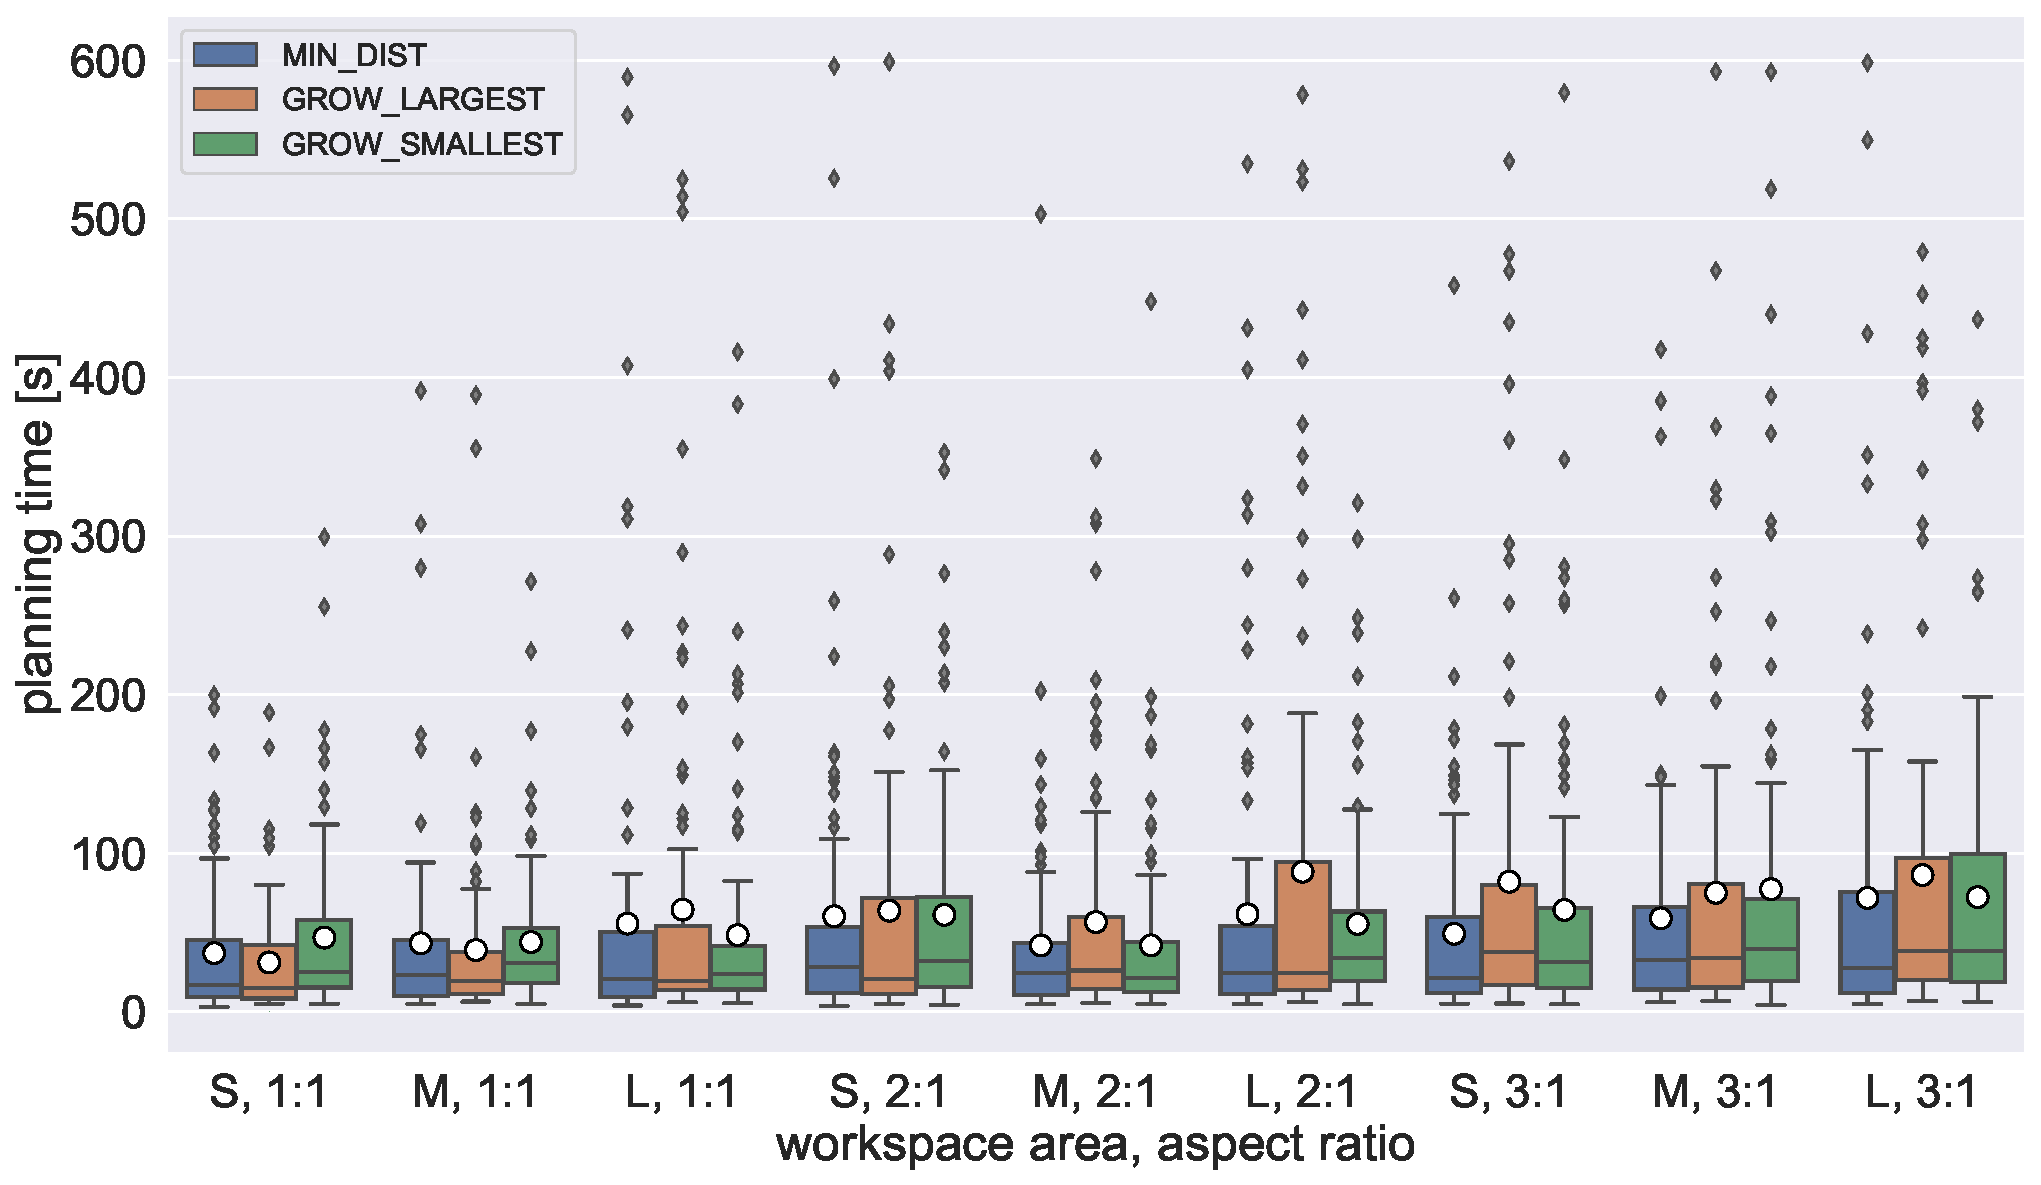
\includegraphics[width=0.9\textwidth]{figures/plots/AFBS_time.pdf}
		\caption{Planning time in seconds. Only plans that did not time out are shown.}
		\label{fig:AFBS_time}
	\end{subfigure}
	
	\begin{subfigure}[b]{\textwidth}
		\centering
		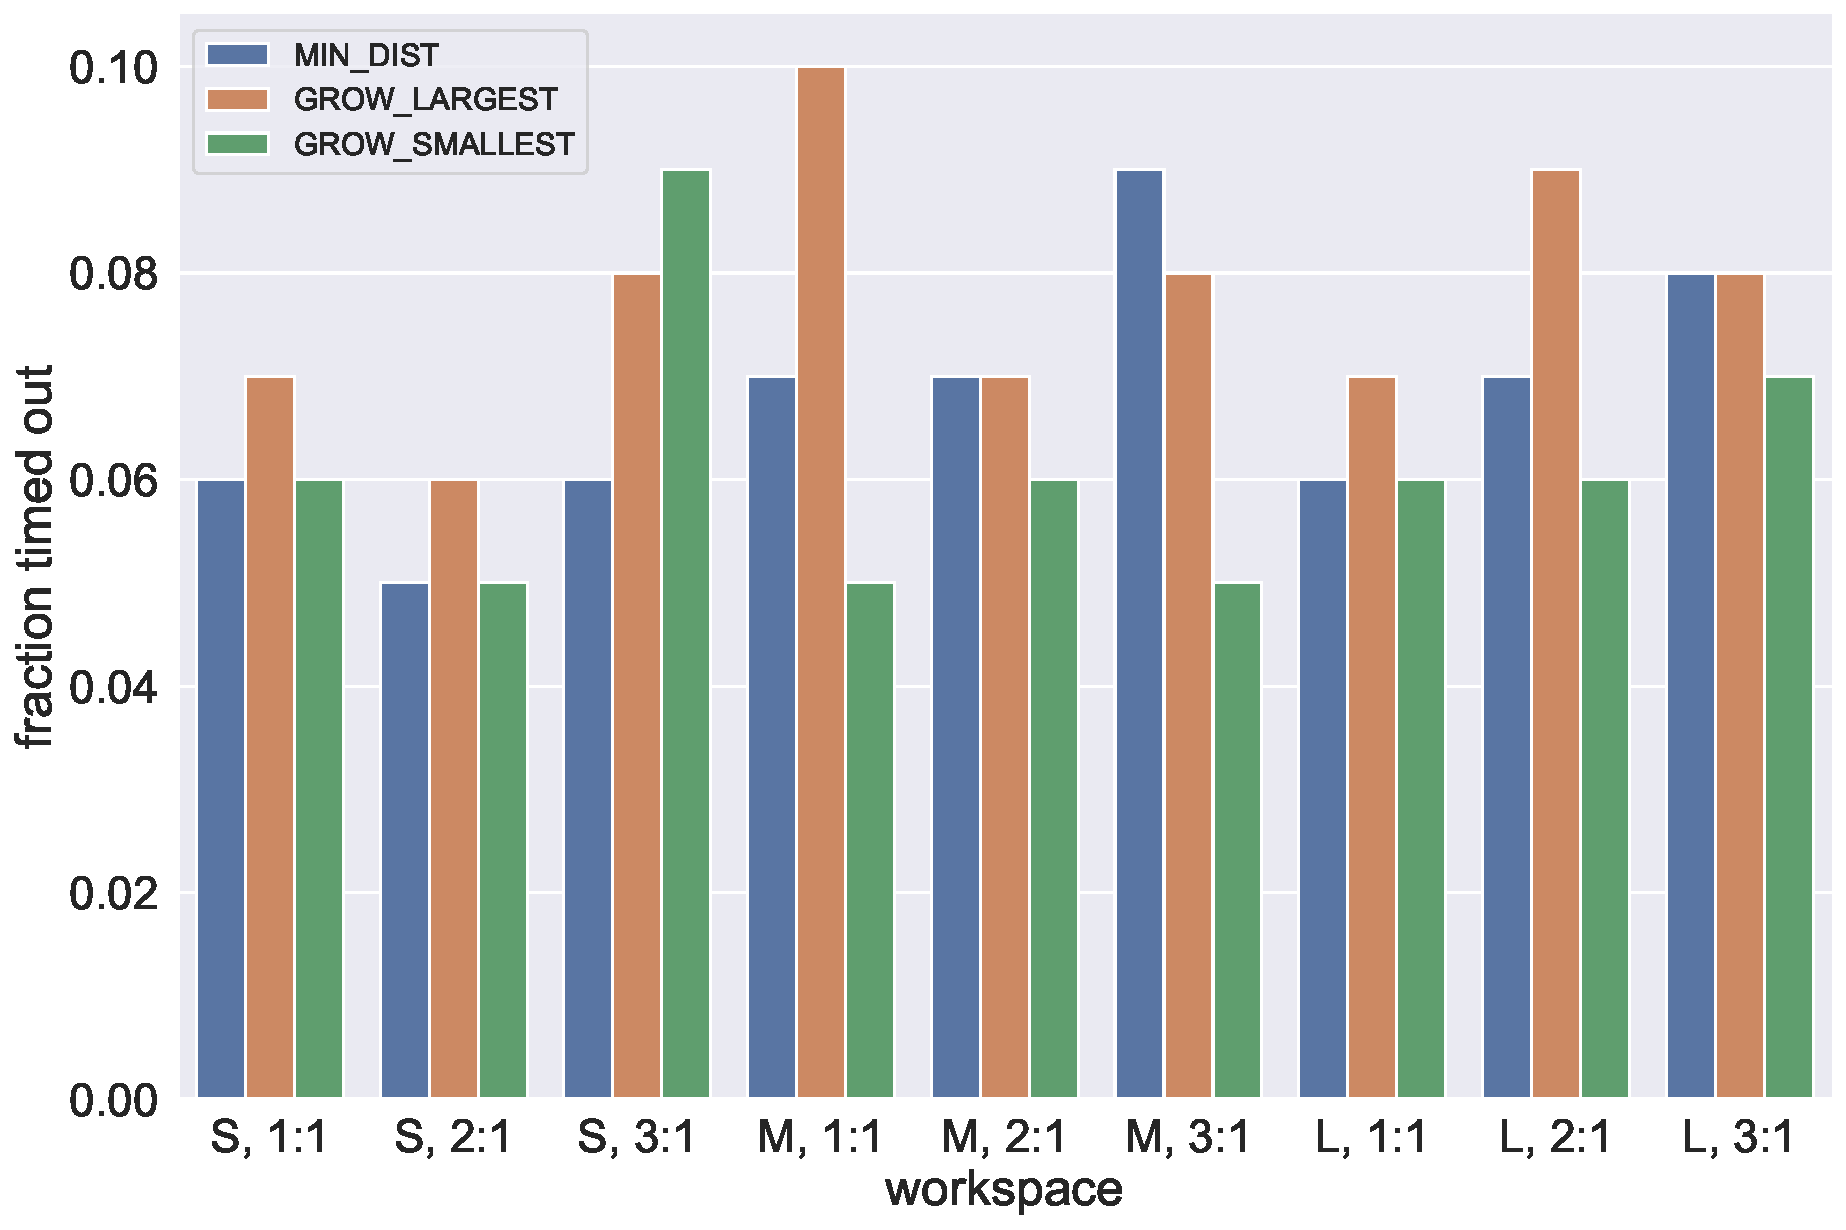
\includegraphics[width=0.9\textwidth]{figures/plots/AFBS_timeout.pdf}
		\caption{Fraction of plans that timed out.}
		\label{fig:AFBS_timeout}
	\end{subfigure}
	\caption[Planning time and fraction timed out for different workspace variations]{Planning time and fraction timed out for different workspace variations listed in \autoref{tab:workspaces}. All option sorting strategies are compared.}
	\label{fig:AFBS_timestats}
\end{figure}

\autoref{fig:AFBS_time} shows the planning time for all workspace variations.
In terms of the size within one class of aspect ration no significant affect can be observed.
Narrowing down the workspace by increasing the aspect ration seems to increase planning time slightly, but for the majority of instances planning time stays under $100$ seconds.
The fraction of timeouts in \autoref{fig:AFBS_timeout} remains constant for all workspaces and the options sorting strategies do not show any difference as well.

\paragraph{Plan Cost} 

\begin{figure}
	\centering
	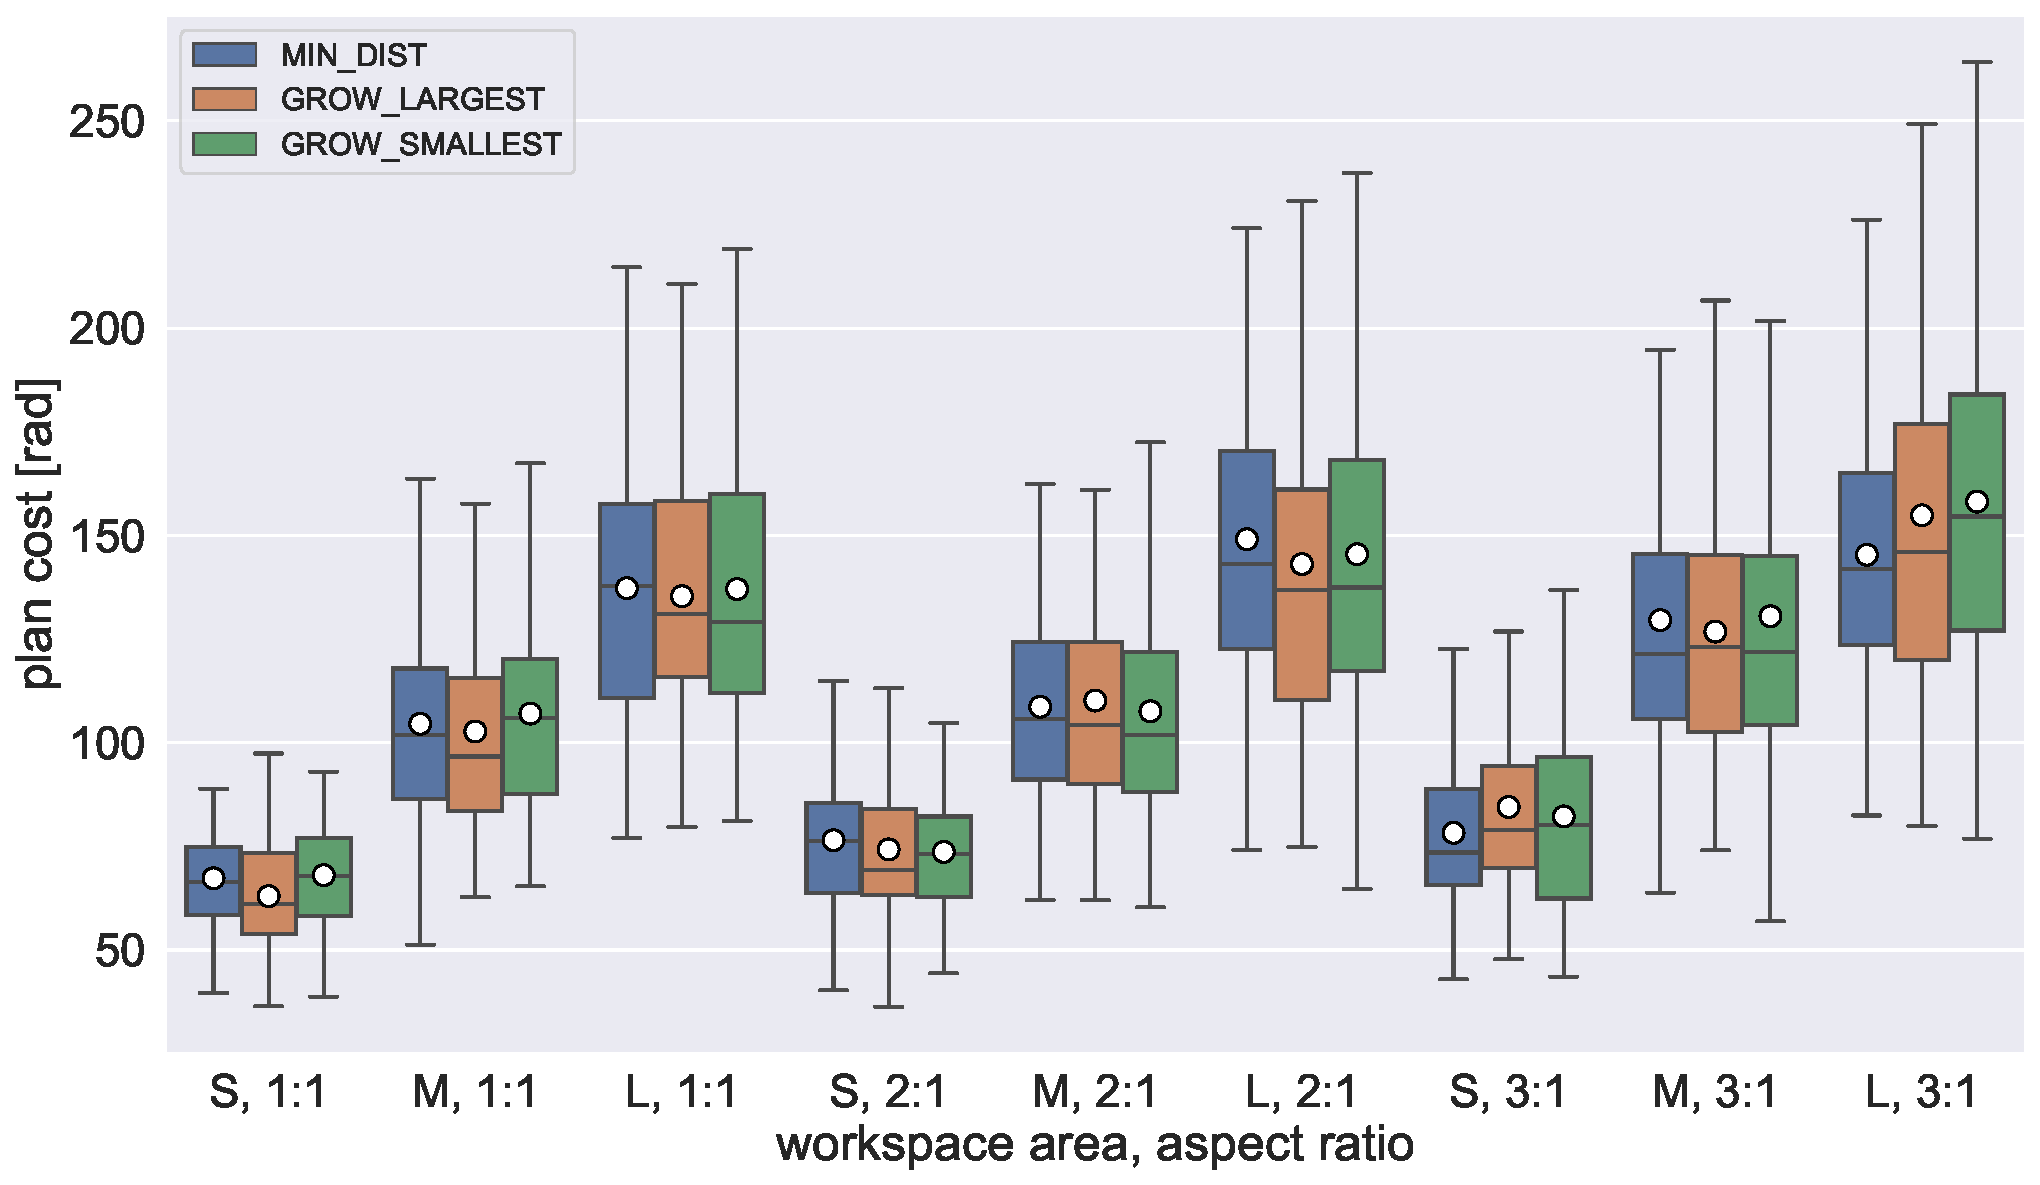
\includegraphics[width=0.9\textwidth]{figures/plots/AFBS_cost.pdf}
	\caption[Plan cost for different workspace variations]{Plan cost in radians of successful plans for different workspace variations with varying areas and aspect ratios. All option sorting strategies are compared.}
	\label{fig:AFBS_cost}
\end{figure}

It is not surprising that the distribution of rotational cost, presented in \autoref{fig:AFBS_cost}, increases with bigger workspace areas.
Cubes and walls are further apart, which results in more pivot walking steps necessary to assemble polyominoes.
With in a class of same size, increasing the aspect ratio results in slightly more rotational cost as well.





\section{Assembly for Red and Blue Cube Ratio}
\label{sec:AFNR}

We examined the affect of red and blue cube ratio on planning time.
For this we increased the number of red cubes $0 \leq n_\textit{red} \leq \lfloor \frac{n}{2}\rfloor$ while keeping the target polyomino size fixed at $n = 10$.
With $n_\textit{red} = 0$ only north-south connections allow the creation of just a vertical line polyomino.
$n_\textit{red} = \lfloor \frac{n}{2}\rfloor$ holds the biggest variety of polyomino shapes.
To exclude the influence of varying polyomino shapes on the experiment, the shape is set to a $10 \times 1$ polyomino.
$\lfloor \frac{n}{2}\rfloor < n_\textit{red} \leq n$ is equal to $0 \leq n_\textit{blue} \leq \lfloor \frac{n}{2}\rfloor$.
Conducting the experiment with $n_\textit{red}$ or $n_\textit{blue}$ in equivalent.
The patterns of red and blue cubes within the $10 \times 1$ polyomino and the initial configurations are randomly generated in a workspace of size $50 r_C \times 50 r_C$.
For each $n_\textit{red}$ $100$ samples were taken.

\paragraph{Planning Time}

\begin{figure}
	\centering
	\begin{subfigure}[b]{\textwidth}
		\centering
		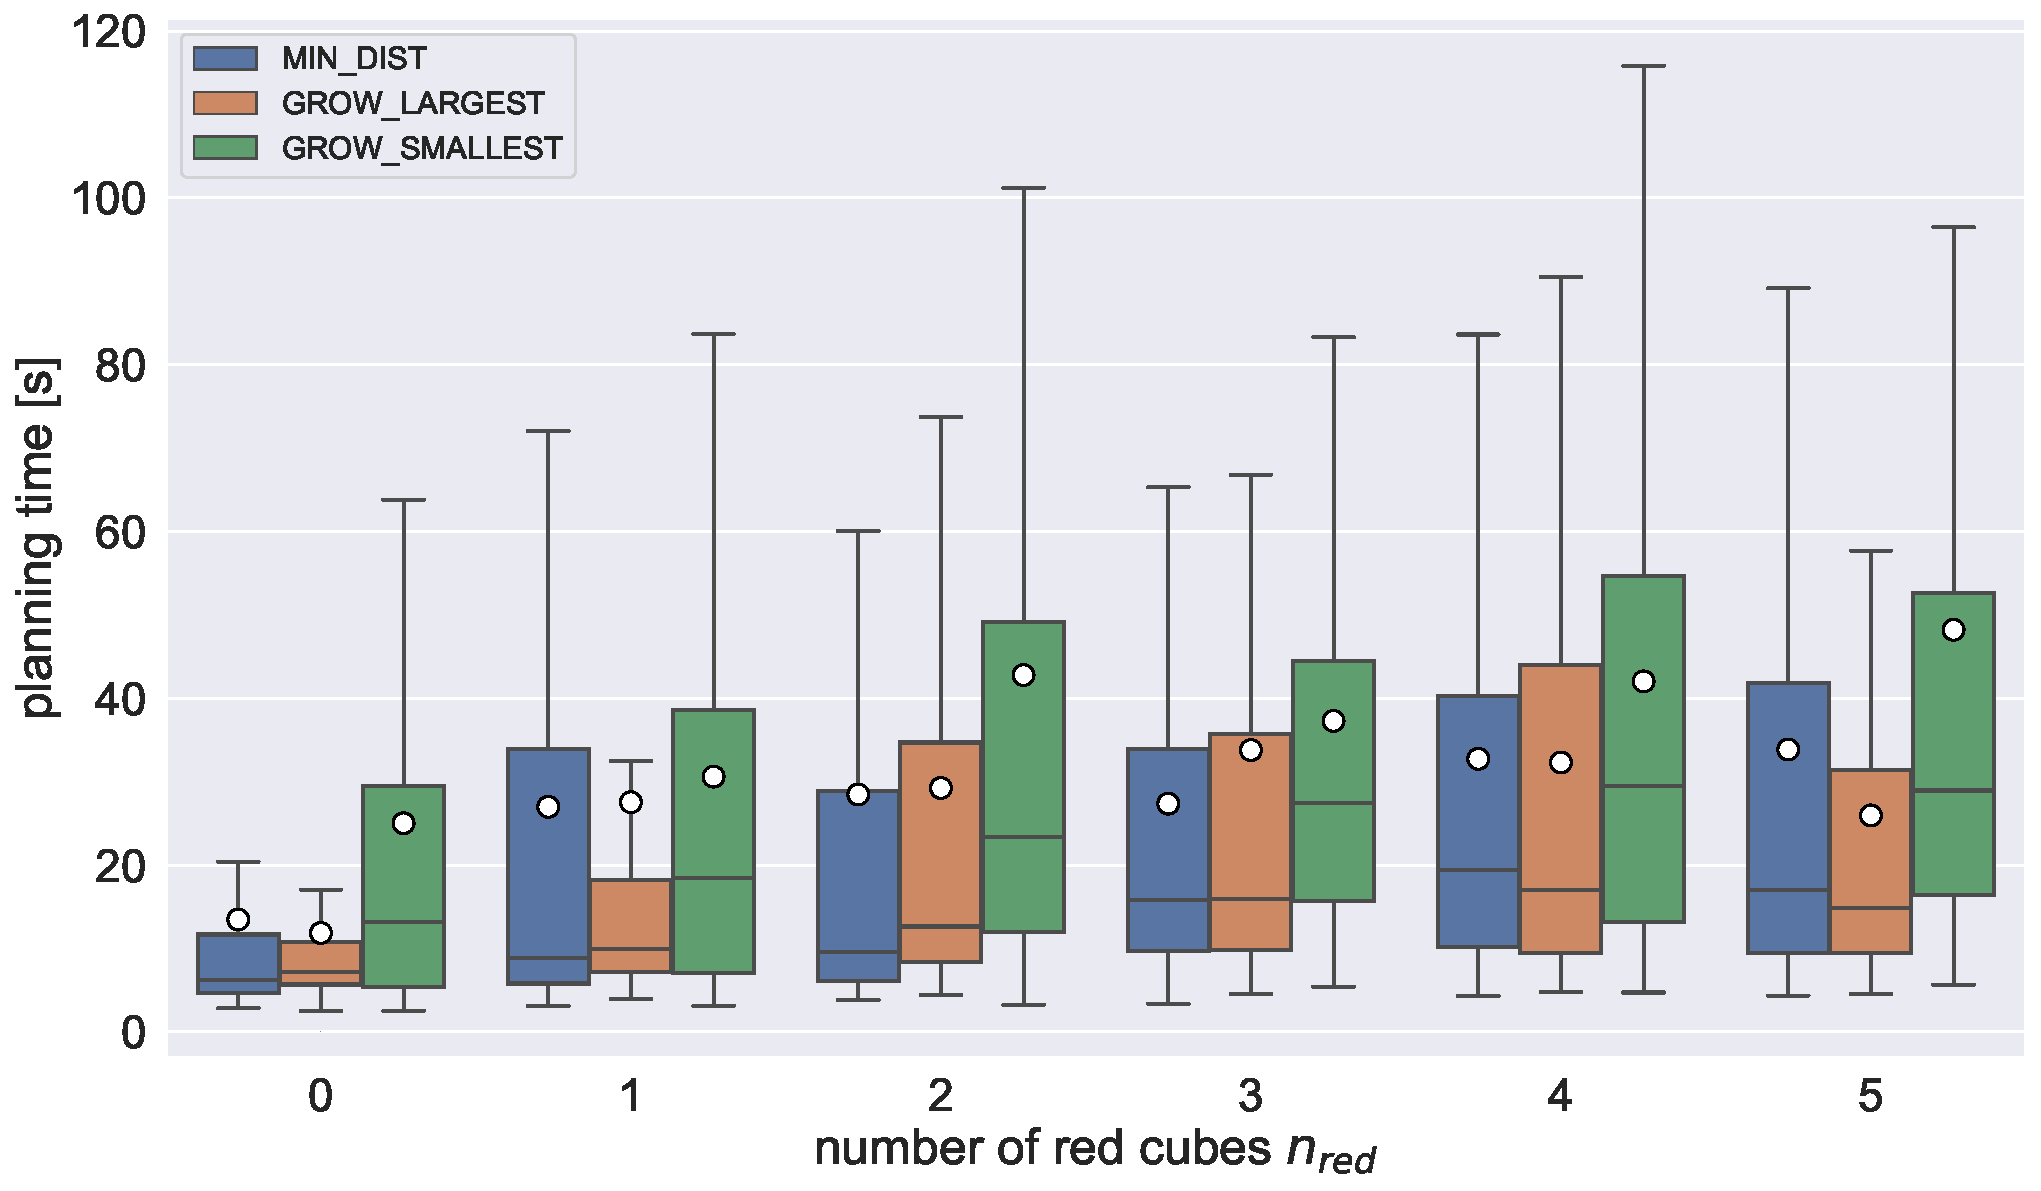
\includegraphics[width=0.9\textwidth]{figures/plots/AFNR_time.pdf}
		\caption{Planning time in seconds. Only plans that did not time out are shown.}
		\label{fig:AFNR_time}
	\end{subfigure}
	
	\begin{subfigure}[b]{\textwidth}
		\centering
		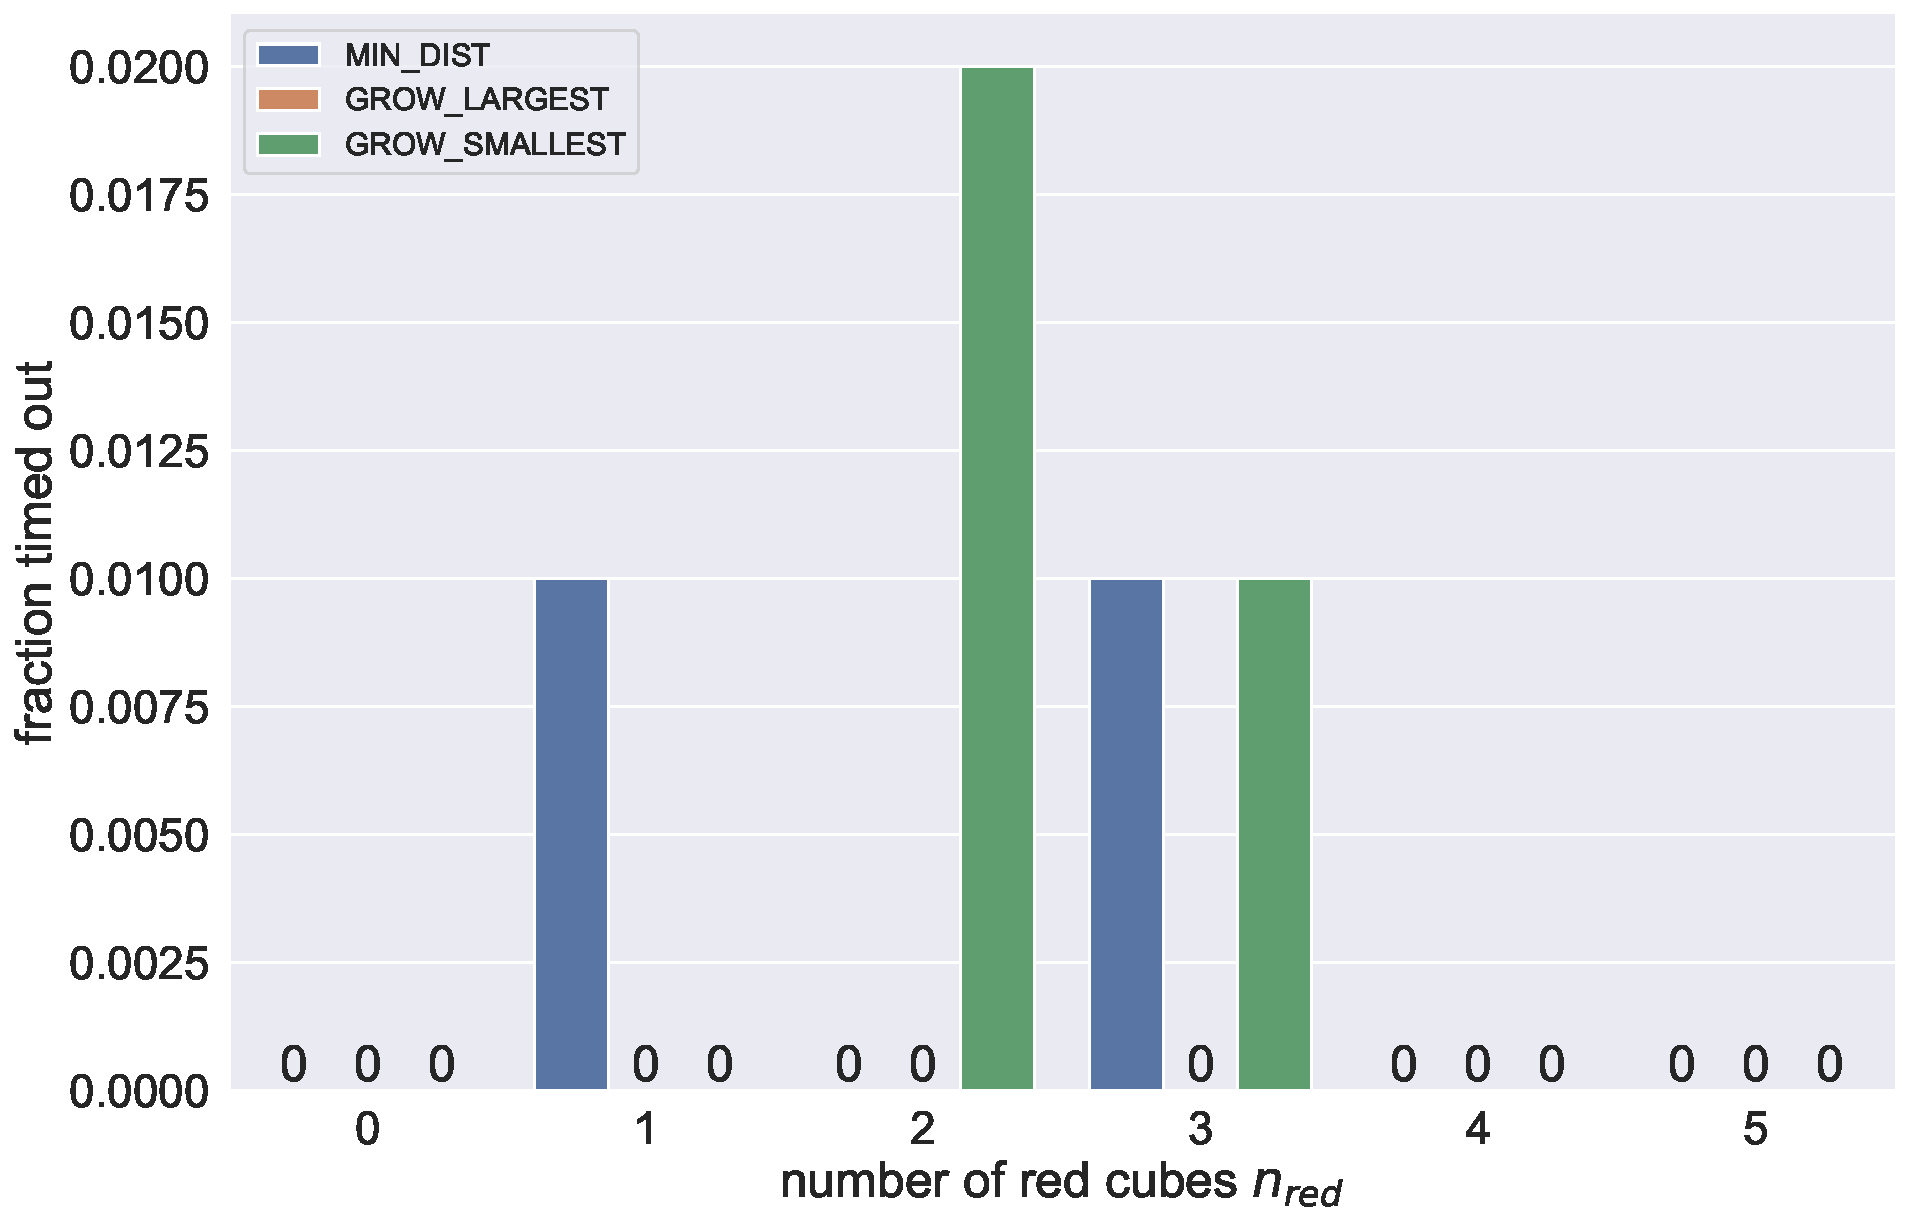
\includegraphics[width=0.9\textwidth]{figures/plots/AFNR_timeout.pdf}
		\caption{Fraction of plans that timed out.}
		\label{fig:AFNR_timeout}
	\end{subfigure}
	\caption[Planning time and fraction timed out for number of red cubes]{Planning time and fraction timed out for different numbers of red cubes $n_\textit{red}$. All option sorting strategies are compared.}
	\label{fig:AFNR_timestats}
\end{figure}

\autoref{fig:AFNR_time} shows the distribution of planning time for this experiment.
By increasing $n_\textit{red}$ from $0$ to $1$ a clear increase in planning time is visible.
With only blue cubes every cube can be placed everywhere in the polyomino.
By introducing one red cube position becomes important.
Further increasing the number of $n_\textit{red}$ does not affect planning time significantly.
For these vertical straight line polyominoes growing the smallest component performs slightly worst than the other two option sorting strategies.
The fraction of timeouts presented in \autoref{fig:AFNR_timeout} is under $2\%$ for all $n_\textit{red}$. 




	\chapter{Conclusion}
\label{chap:conclusion}

In this thesis we developed a heuristic approach for the motion planning problem of assembling polyominoes with magnetic modular cubes \cite{Bhattacharjee2022} in the 2-dimensional special Euclidean group $\textit{SE}(2)$.

All thought our simulator is not a physically accurate representation of magnetic modular cubes, since we are simulating 3D-movement in a 2D-environment, it is able to depict continuous movement of rotations and pivot walking and also simulates magnetic attraction and repulsion of embedded permanent magnets.
While doing so, collision between cubes and collision with workspace boundaries is detected and resolved.

These attributes of the simulator allow our closed-loop local planning algorithm to dynamically adjust for events like structures blocking each other, structures sliding along the workspace boundaries and varying movement directions due to different pivot walking displacement vectors of polyomino shapes.
By not limiting rotations to certain degrees, structures can always be aligned and theoretically connect by pivot walking a straight path.
Above mentioned events prevent this straight and optimal movement, but dynamic realigning provides a good heuristic for minimizing movement while being efficient on planning time.

We constrained the workspace to be rectangular with no obstacles expect the outer boundaries and experimented with different sizes and aspect ratios of the rectangle.
Our local planner is not designed to handle obstacles.
Designing a local planner able to navigate around obstacles and handle pivot walking displacement and sliding on walls in a more calculated way, could be a interesting direction for future work.

The simulator is balanced between physical accuracy and efficiency, but it remains a high fidelity physics simulation.
Simulating movement is costly and local plans require planning times in a range of seconds.
On a global scale of doing multiple local plans to assemble desired target structures, simulation should be avoided as much as possible.
Using classical motion planning approaches that broadly explore the configuration-space like RRT, are not feasible under this condition.

Our global planner uses the ability of two-cutting polyominoes to create a two-cut-sub-assembly graph that will be used as a building instruction for target polyominoes.
The configuration-space is explored by depth first search traversing this graph, to get closer to the target with each local plan.
The graph leaves multiple options for traversing one edge, because it does not consider workspace position of polyominoes. 
We evaluated three strategies of sorting these options by best probable outcome.

The global planner can identify if the assembly of a target is possible out of any sub-assemblies present in the workspace at any point in time, but requires equal amounts of cubes in the workspace and in the target polyomino.
How to work with more cubes than necessary for the assembly when two-cut-sub-assembly graphs are used remains an open question for future work.

We evaluated the assembly of polyominoes with up to 12 cubes in varying shapes and patterns of cube types.
Planning time and timeout failures increase exponentially with the number of cubes, as it is expected with increasing dimensionality of the configuration-space.
We are able to solve the majority of instances in under $200$ seconds, but certain attributes of polyominoes heavily decrease efficiency of the global planner.
We found out that a combination of many connections within a polyomino and polyomino width produces especially bad results.

The option sorting strategies seem to perform differently for varying shapes, but we were not able to identify a clear pattern.
Studying attributes of polyominoes and their effect on performance is another possible direction for future work.
Designing new specialized option sorting strategies and determining which on to use, based on the target polyomino, looks promising. 



	
	\bibliographystyle{abbrv}
	\bibliography{bibliography.bib}

\end{document}